\chapter{Extended Structures of Nonmetallic Elements}

In this chapter, we will consider the bonding of nonmetallic elements
with at least three atoms.  For molecular crystals, see Chapter 9, 
Section 9.4.

\section{The Nitrogen Column}

\subsection{M$_4$}

Three elements of the N column, P, As, and Sb, exhibit stable M$_4$ molecules 
with a tetrahedral configuration
\begin{equation}
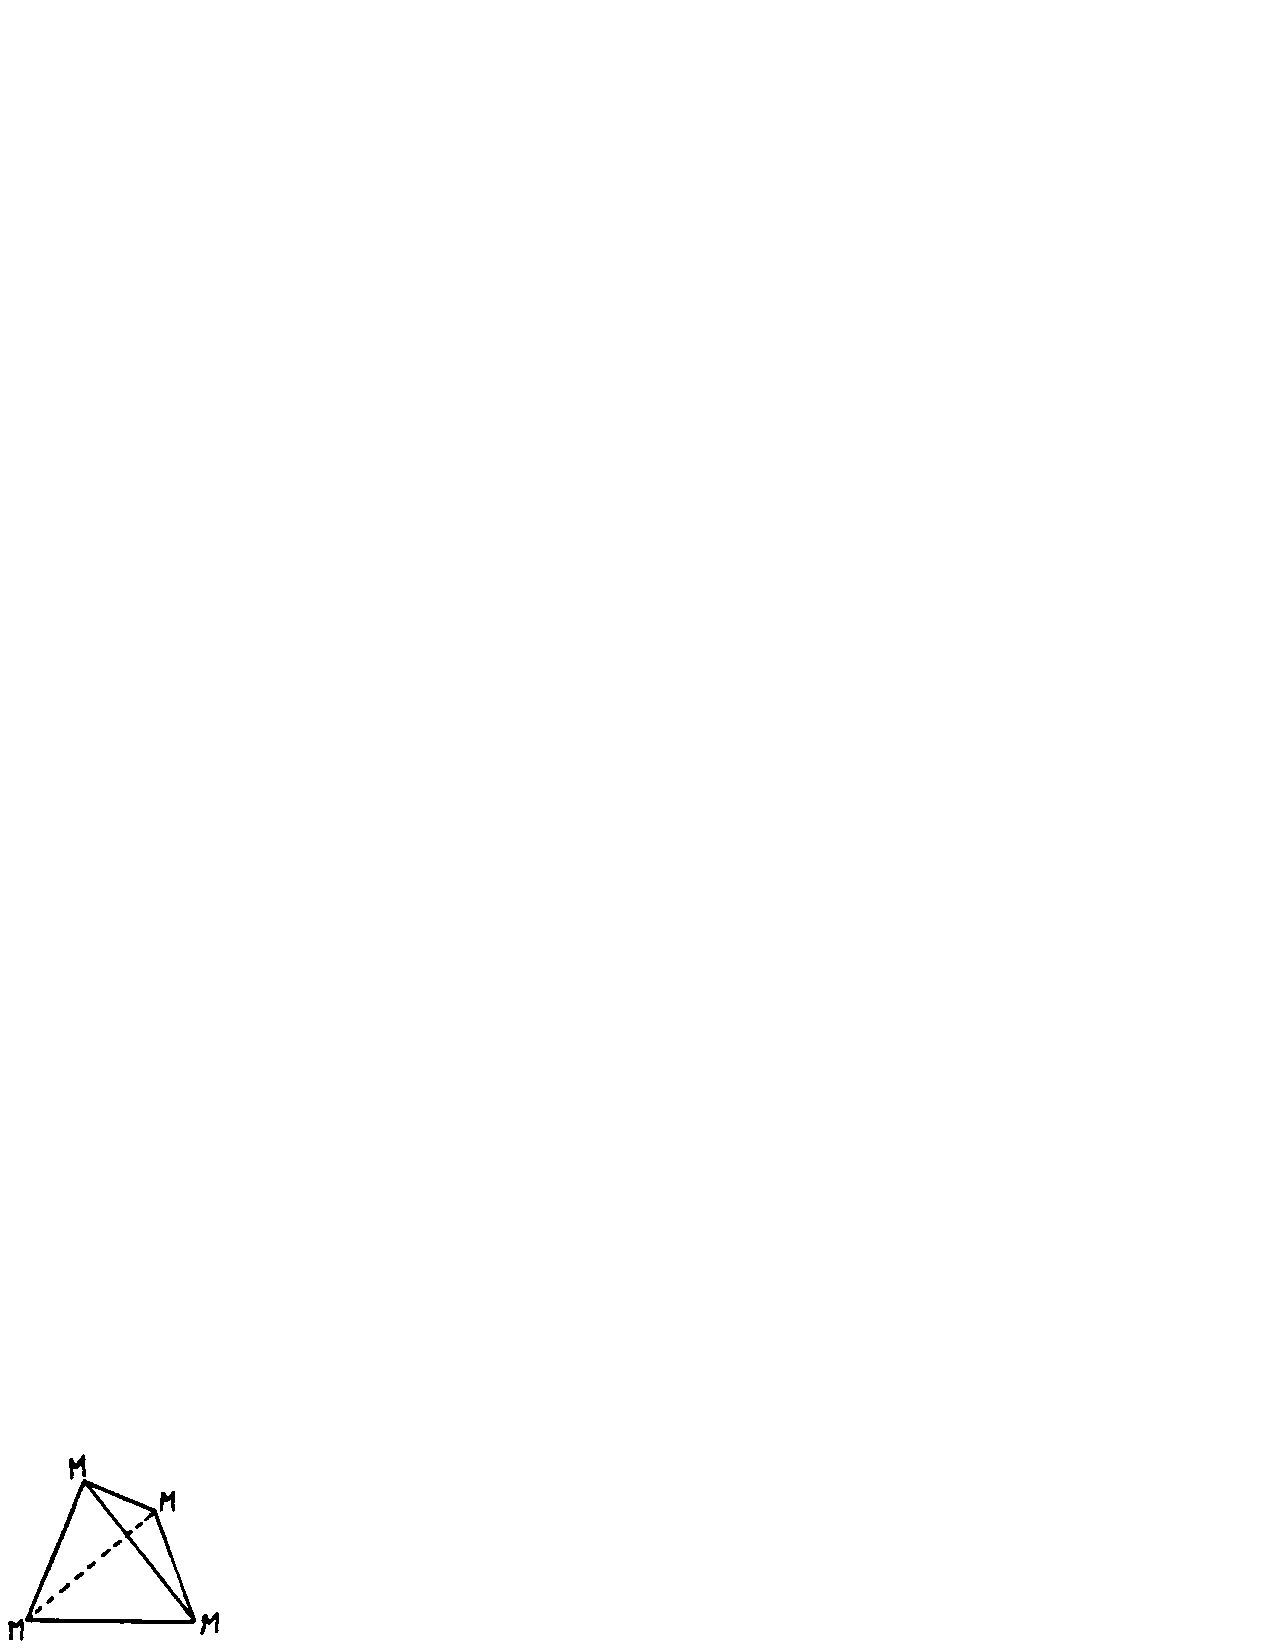
\includegraphics{fg12-01}
\end{equation}
Clearly, these molecules have three single bonds to each atom with the lone 
pairs protruding away from the tetrahedron.  The bond angle here, 
60$^{\circ}$, is less than the ideal one for $p$ bonds, 90$^{\circ}$. This
suggests that the bond orbitals on each M point are slightly away, 
19.47$^{\circ}$, from the adjacent As, so
that each $p$ orbital is at 90$^{\circ}$
\begin{equation}
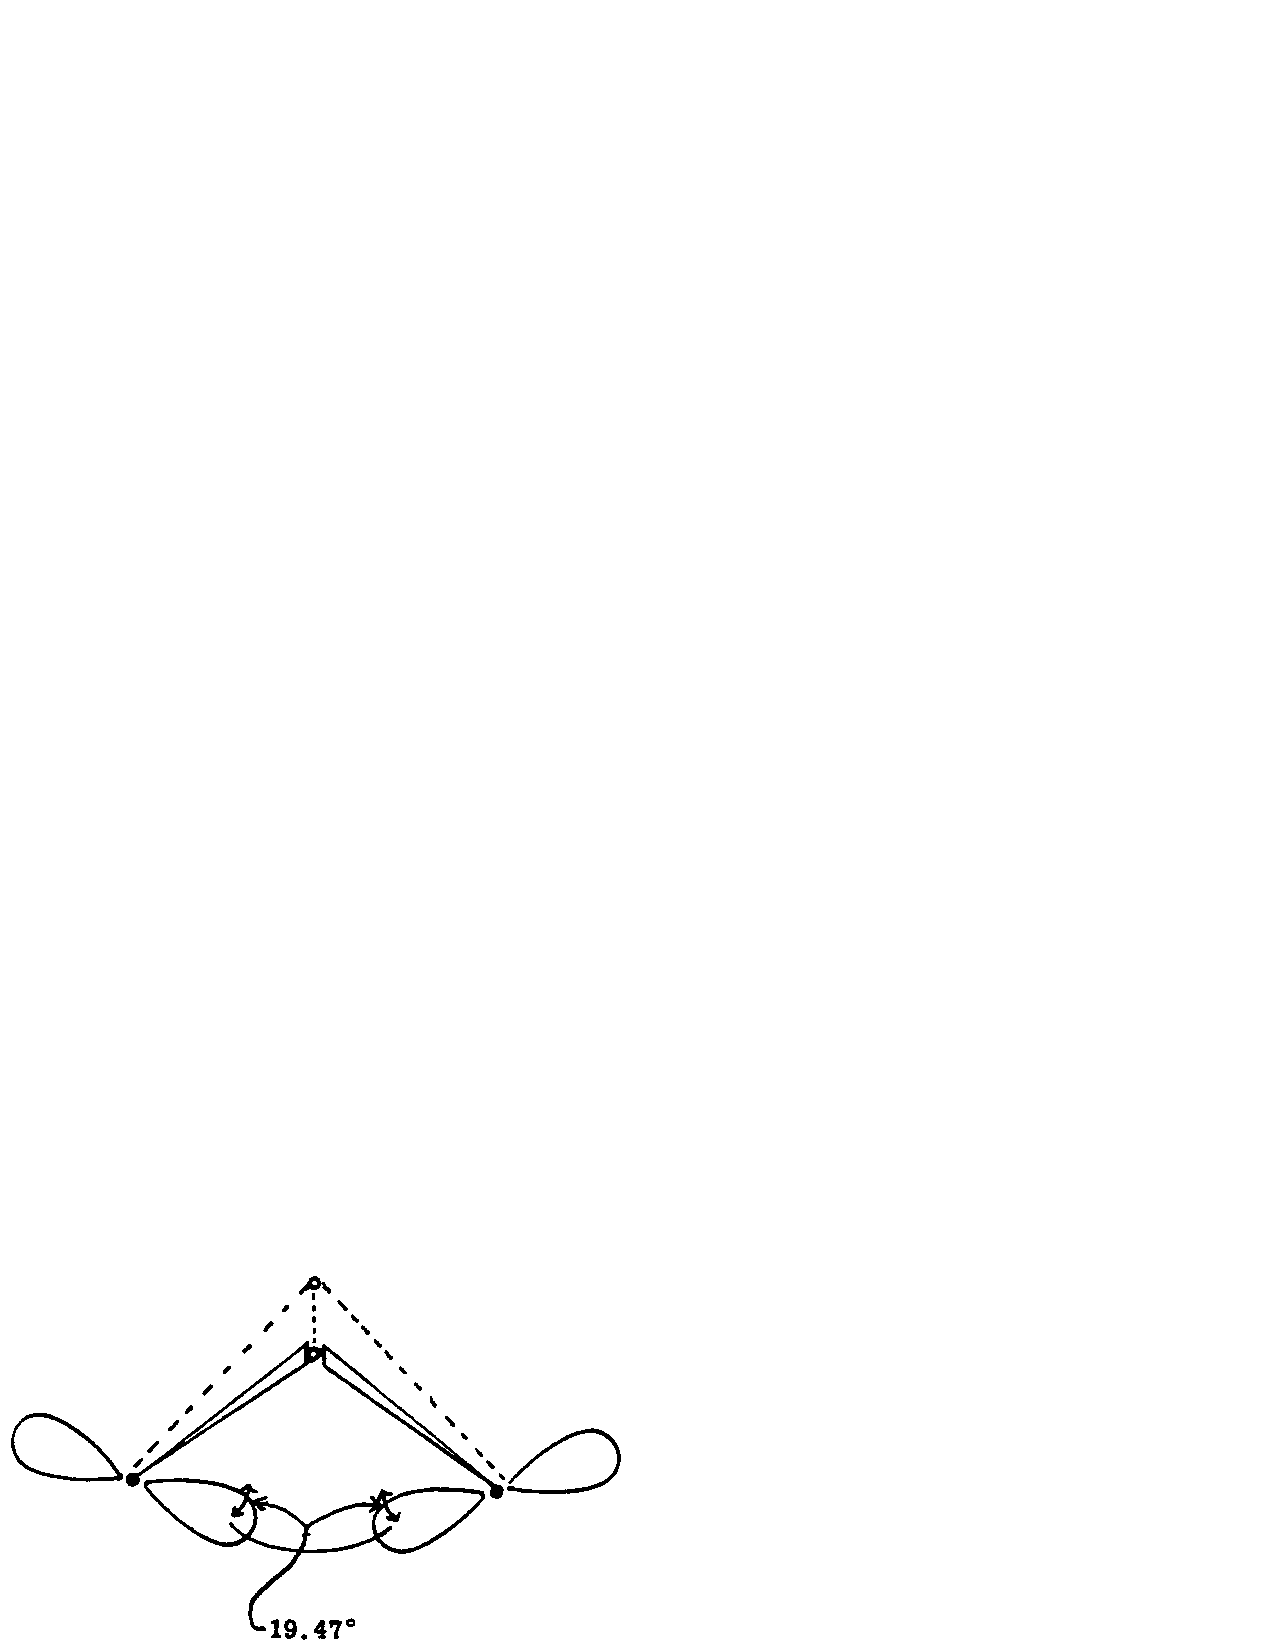
\includegraphics{fg12-02}
\end{equation}
Considering M$_4$ to have six single bonds leads to the average single
bond energies in Table \ref{chap12-tab1}.  Comparing to M $\equiv$ M,
we see that the strength of a pi bond ranges from 73 percent of the
sigma bond for P to 40 percent for Bi.  As a result, the M$_4$ species
is considerably more stable, by 54 to 72 kcal, than two M$_2$ species.
As a result, the vapor of the solid is primarily M$_4$ up to very high
temperatures as indicated in Table \ref{chap12-tab2}.  For example the
vapor over Sb at the melting point is 97 percent Sb$_4$ and 3 percent
Sb.  Sb$_4$ is the predominant species up to $\sim$1350 K.  Even at
the boiling point, 1860 K, there is 83 percent Sb$_2$, 13 percent
Sb$_4$, and 4 percent Sb.

\begin{table}
\caption{Bond energies, in kcal, for N column species.$^d$}
\label{chap12-tab1}
\begin{tabular}{ccccccccc}\\ \hline
&\multicolumn{3}{c}{Single}&Double&Triple$^e$&Two&Ratio\cr
&Solid$^h$&M$_4$$^i$&H$_2$M$-$MH$_2$&HM-MH&M$\equiv$M&$\pi^g$&$\pi$ to 
$\sigma$&$2E(M_2)-E(M_4)$\cr

N & & (52)$^f$ & 55.4$^b$ & 129.0$^b$ & 225 & 173 & (1.7) & 
($-$138)\cr
P & 56.4$^c$ & 48.1$^b$ & 51$^{b,d}$ & & 116 & 69 & 0.73 & 54.05\cr
As & 48.2 & 42.1 & & & 91 & 49 & 0.58 & 71.8\cr
Sb & 41.8 & 33.4 & & & 71 & 38 & 0.56 & 63.32\cr
Bi & 33.0 & (26)$^a$ & & & 47 & 21 & 0.40 & (64)\cr
\hline
\end{tabular}\\
$^a$ For P, As, and Sb, the solid has a cohesive energy 8.0, 6.1, 
and 7.4 kcal larger than that of M$_4$.  We estimated the bond energy for 
Bi$_4$ by assuming that this 7.0 kcal difference still applies.
$^b$ Reference 6.
$^c$ Based on black P.
$^d$ Based on reference 1, unless otherwise noted.
$^e$ Chapter 8.
$^f$ Based on the bond energy of $H_2N-NH_2$ corrected 
for the difference between $H_2P-PH_2$ and $P_4$.  Probably $N_4$
would lead to an even weaker bond due to the small bond angle and high 
strain energy.
$^g$ $D(M \equiv M) - D ( M - M )$.
$^h$ In average.  In the solid, there are three short bonds 
to each atom. In calculating the
average bond energy, we have assumed that all the bonding is associated
with these three bonds.  This is an over-estimate since there are other
attractive interactions.
$^i$ Neglecting any strain energy in M$_4$.
\end{table}



\begin{table}
\caption{Composition of vapor.$^a$}
\label{chap12-tab2}
\begin{tabular}{ccccc}\\ \hline
& &\multicolumn{3}{c}{Fraction}\cr
& T(K) & M & M$_2$ & M$_4$\cr

P & 704 (bp) & $4 \times 10^{-15}$ & $4 \times 10^{-5}$ & 1.000\cr
As & 876 (bp)$^b$ & $1 \times 10^{-11}$ & $2 \times 10^{-5}$ & 1.000\cr
Sb & 298.15 & 0 & 0 & 1.000\cr
& 904 (mp) & 0 & 0.032 & 0.966\cr
& 1860 (bp) & 0.045 & 0.827 & 0.128\cr
Bi & 298.15 & 0.649 & 0.351 & 0\cr
& 544.52 (mp) & 0.238 & 0.762 & 0\cr
& 1837 (bp) & 0.535 & 0.465 & 0\cr
\hline
\end{tabular}\\
$^a$ Reference 2.
$^b$ Also, $5 \times 10^{-6}$ for As$_3$.
\end{table}

The molecule H$_2$P$-$PH$_2$ leads to a PP bond energy of 51 kcal, in reasonable 
agreement with the value
48.1 kcal from P$_4$.  Thus, we might use the bond energy of 
H$_2$N$-$NH$_2$, 55.4 kcal, to estimate the energy of a hypothetical 
N$_4$ species.  The 
result is a prediction that N$_4$ is
138 kcal higher in energy than two N$_2$ molecules.  It is not surprising 
that tetrahedral N$_4$ has not
been observed!  Thus, for both N and O the stable form is the diatomic 
molecule with strong pi bonds,
whereas for the other rows of these columns the stable form involves a 
network consisting only of sigma
bonds. In both cases, the first raw element leads to pi bonds stronger than 
the sigma bond, whereas this
relationship is reversed for the other rows. 

\subsection{Crystals}

All crystalline forms of P, As, Sb, and Bi lead to structures with three 
short bonds to each atom.

The metallic form of As, Sb, and Bi has a rhombohedral structure in 
which a bilayer of covalently bonded atoms
\begin{equation}
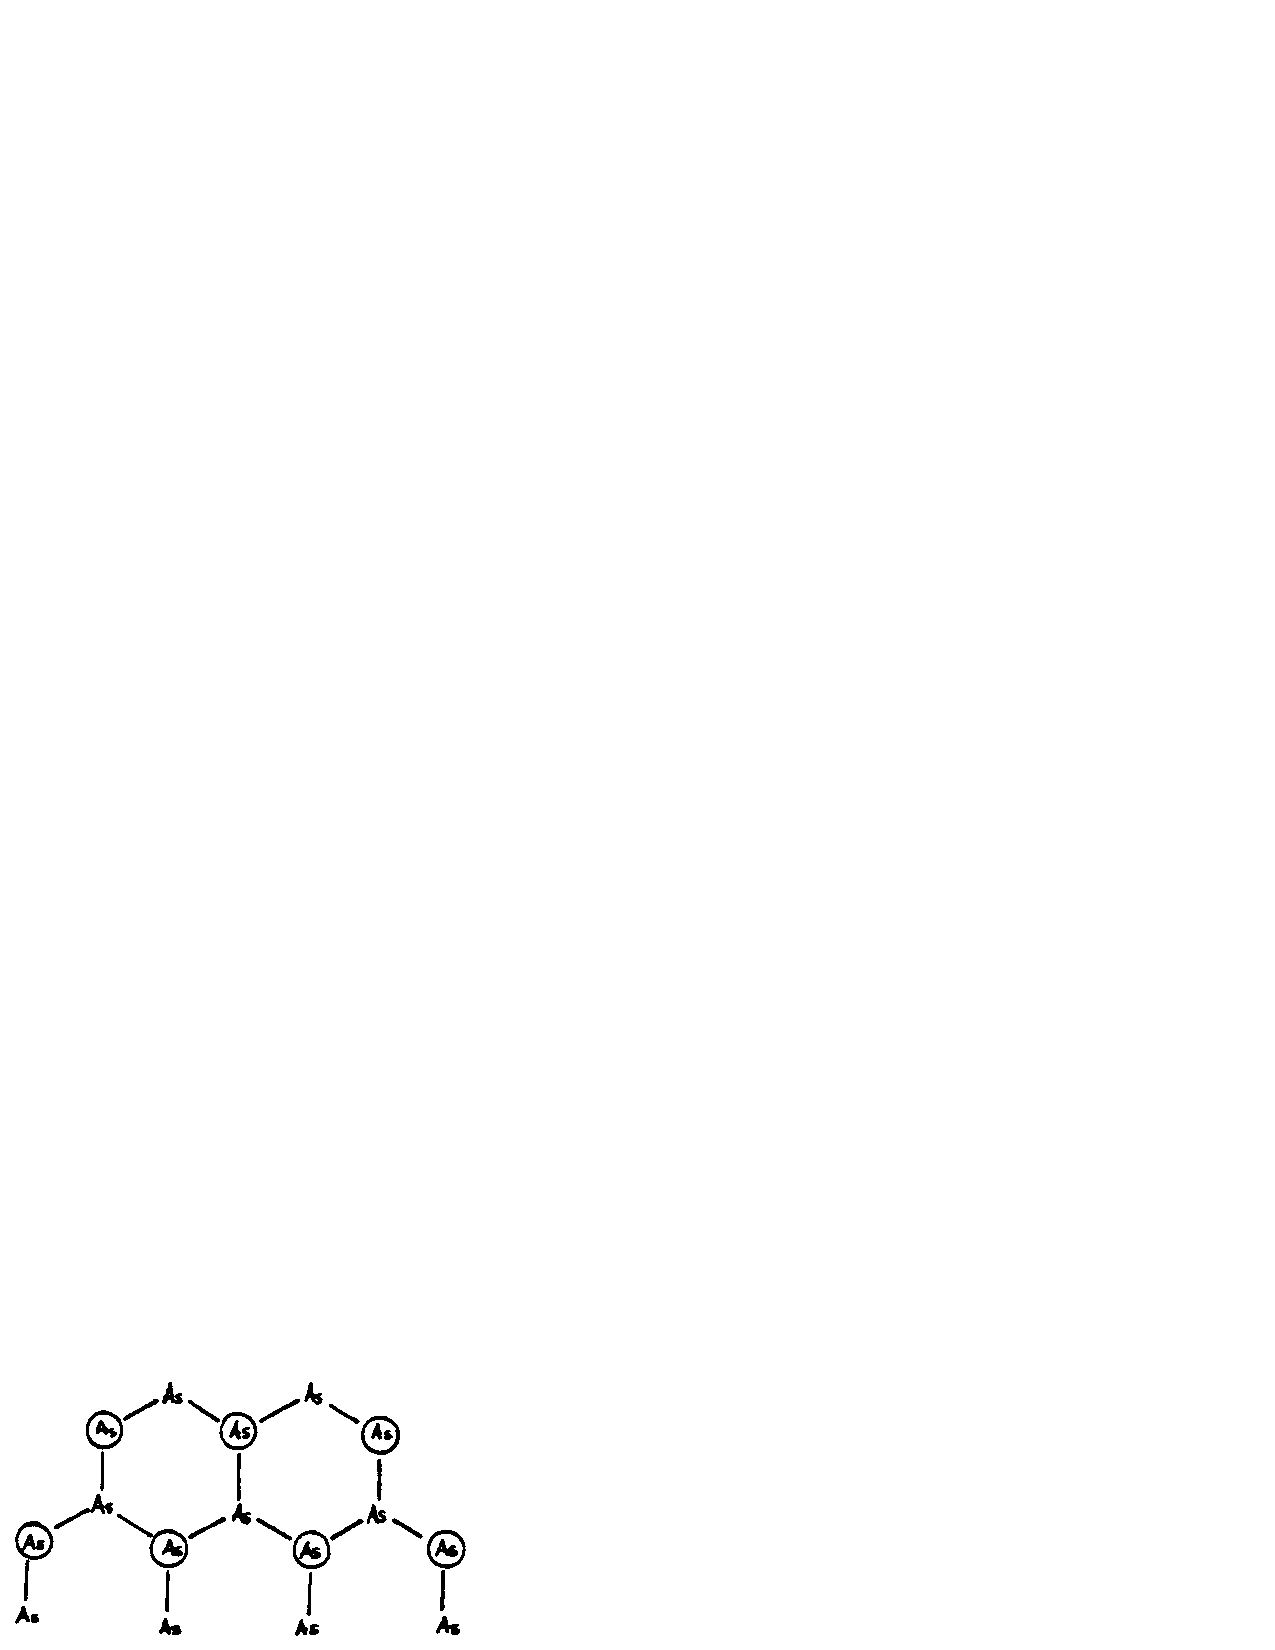
\includegraphics{fg12-03}
\end{equation}
is bonded to adjacent bilayers by three longer, but strong, bonds.
The top atom of one bilayer is positioned below the three bottom atoms
of the next bilayer.  This is the stable crystalline form for all
three elements.  Bond parameters are in Table \ref{chap12-tab3}.

\begin{table}
\caption{Strong and weak bonds.}
\label{chap12-tab3}
\begin{tabular}{cccc}\\ \hline
&\multicolumn{2}{c}{Strong} & Weak\cr
& Angle & Length & Length\cr

P (black) & 100.2$^a$ & 2.234 $\pm$ .014 & 3.592 (two)\cr
As & 90.0 & 2.51 & 3.120\cr
Sb & 95.6$^{\circ}$ & 2.908 & 3.355\cr
Bi & 95.5$^{\circ}$ & 3.072 & 3.529\cr
\hline
\end{tabular}\\
$^a$ Average.
\end{table}

The stable form of P, black P, has a layer structure involving chains of P 
bonded covalently to adjacent chains
\begin{equation}
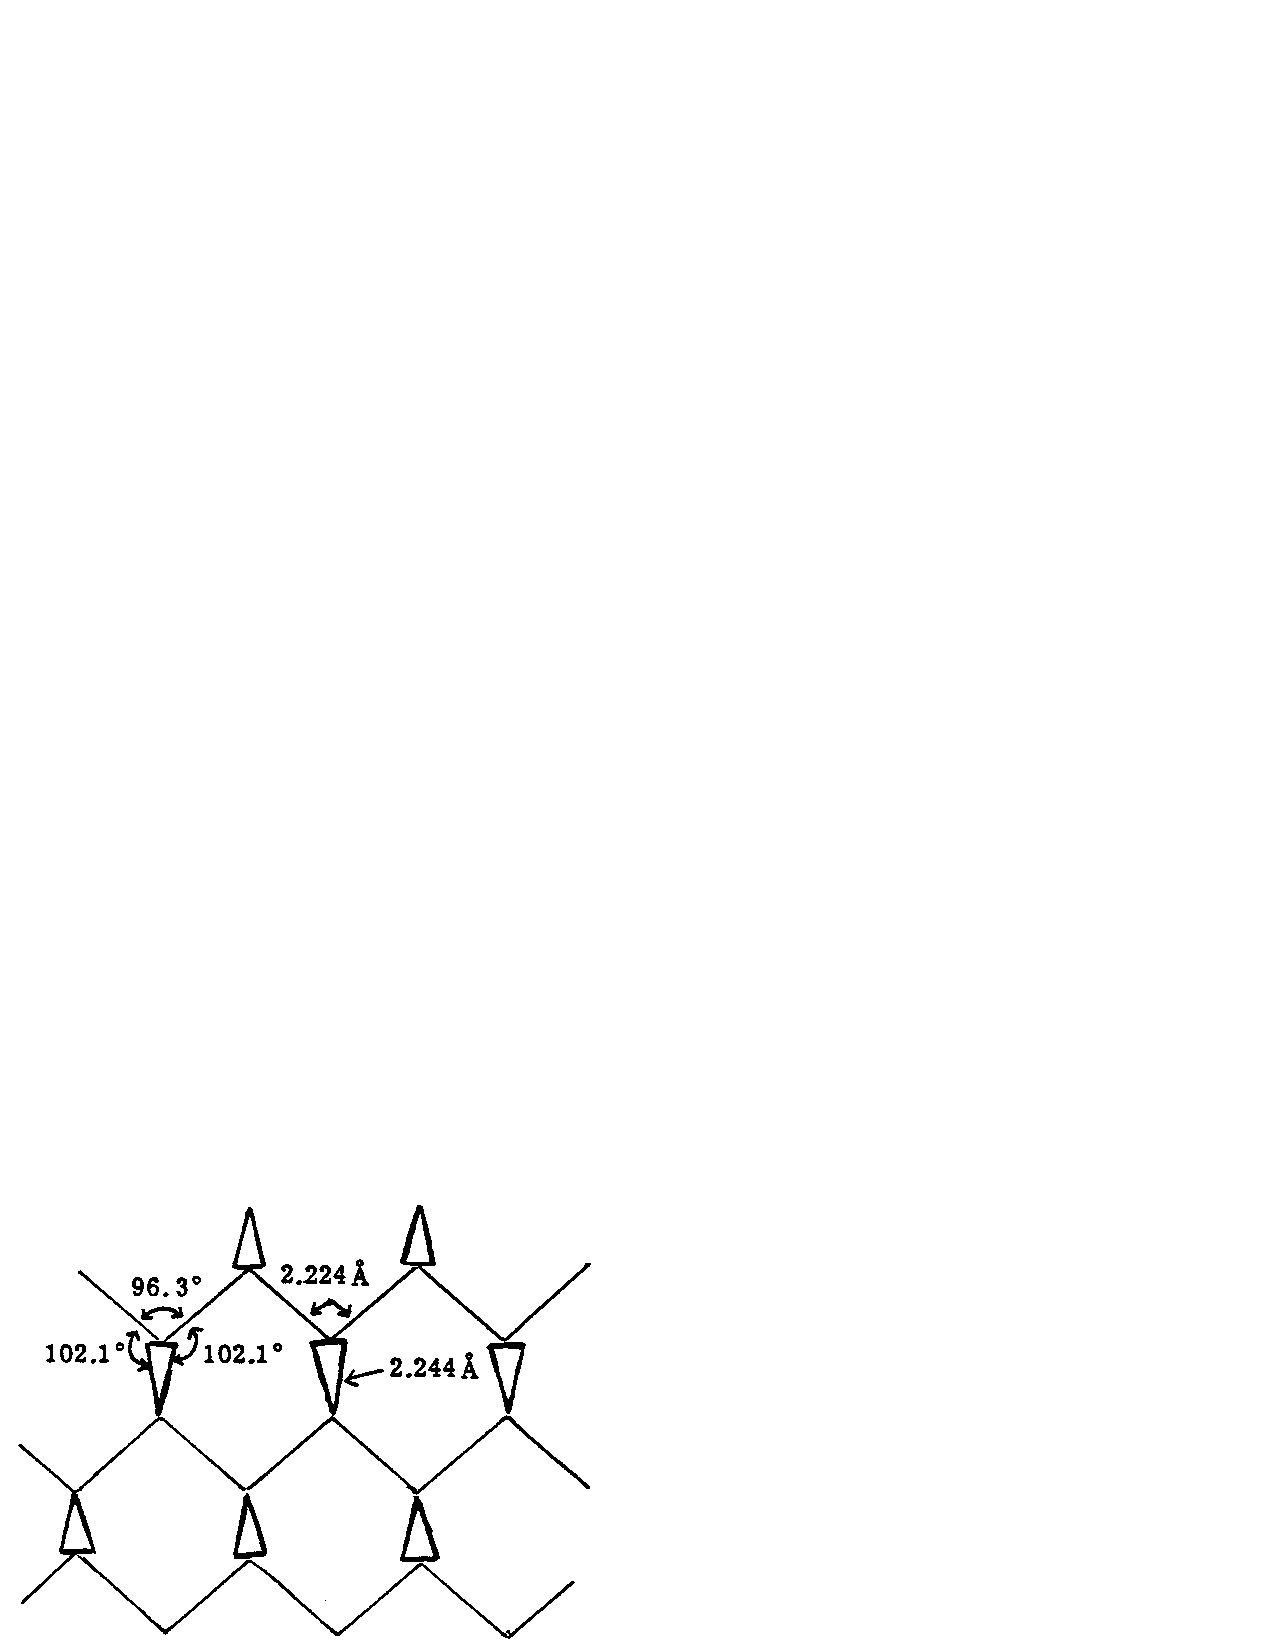
\includegraphics{fg12-04}
\end{equation}
Although most stable, this form is hard to make.  This form resembles that 
of rhombohedral As except that the bond lengths are not all equal.  The 
reference state of P for the JANAF thermochemical tables is red P which 
involves a very complicated layered structure having a P-P bond length 
of 2.22 \AA\ and a bond angle of 101$^{\circ}$.

Condensation of P from the vapor leads to white, or yellow, P, the 
alpha form, consisting of P$_4$ molecules with a bond distance of 
2.21 \AA, weakly bonded to each other.  The form is taken as the
reference state for most thermochemical tables.  Yellow As and yellow Sb 
probably also involve isolated M$_4$ molecules bonded together in the 
crystal.  An interesting form of P is Hittorf's phosphorous, a violet, 
monoclinic substance made by heating red P to 550$^{\circ}$C.  This has 
channels consisting of units of P$_8$ and P$_9$ 
\begin{equation}
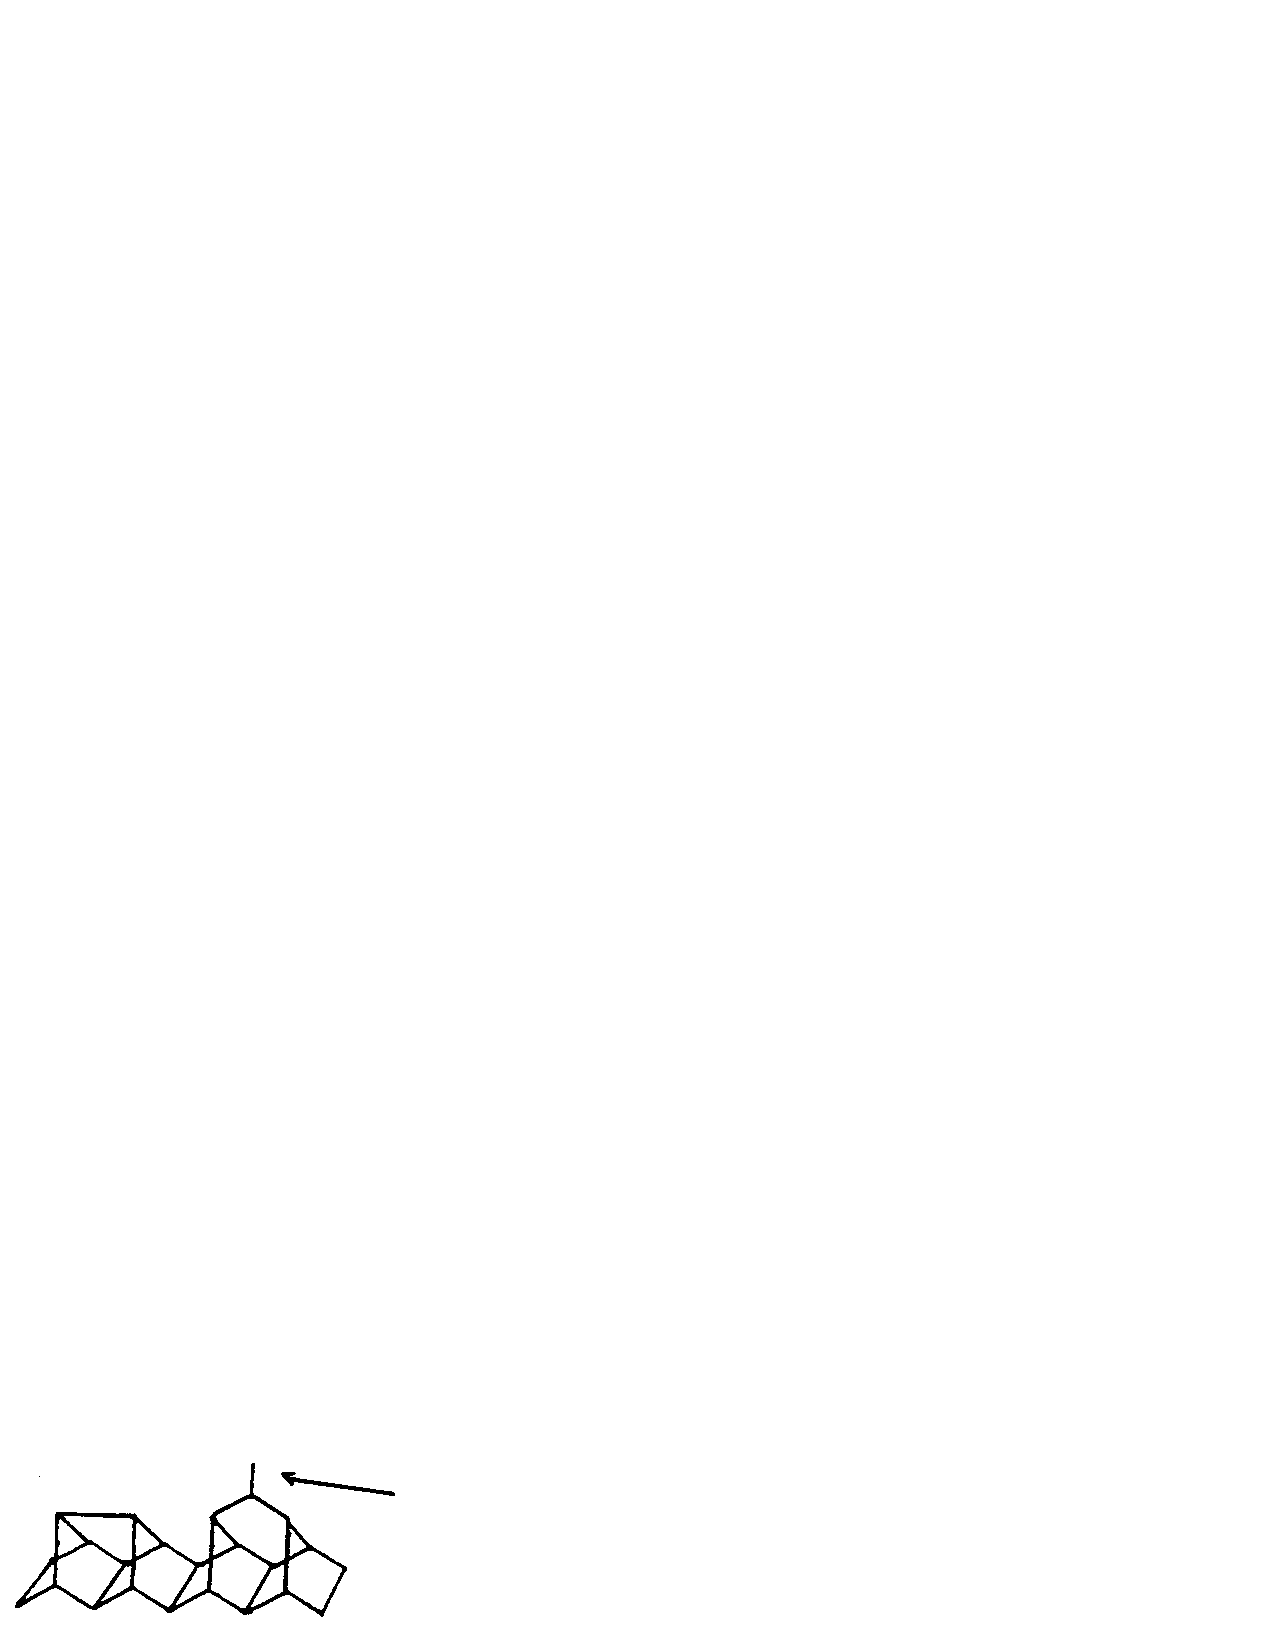
\includegraphics{fg12-05}
\end{equation}
coupled to adjacent channels.  The average PP bond length is 2.219 \AA\ and the 
bond angle is 100.9$^{\circ}$.

Compressing black P to 83 kbar leads to a rhombohedral form like that of As 
and compressing to 111 kbar leads to simple cubic P, with six bonds of 
2.377 \AA.  Condensing As vapor onto a cool surface, leads to yellow As 
analogous to white P, with As$_4$ units.  There is also a rhombic form of 
As analogous to black P.  If the surface is heated to 100$-$200$^{\circ}$C one
gets amorphous As with As-As = 2.94 \AA\ and bond angle 100$^{\circ}$.
Sb also forms an amorphous phase but not Bi.

We see that P, As, and Bi exhibit a dominance of the expected trivalent 
character in the condensed phases but with increase in other bonding 
effects as we proceed down the column.

\subsection{Azides}

As found above, N-N pi bonds are considerably stronger than N-N sigma 
bonds.  Thus, the simplest N
polymers are quite different from those of P, As, etc.

An interesting species would be
\begin{equation}
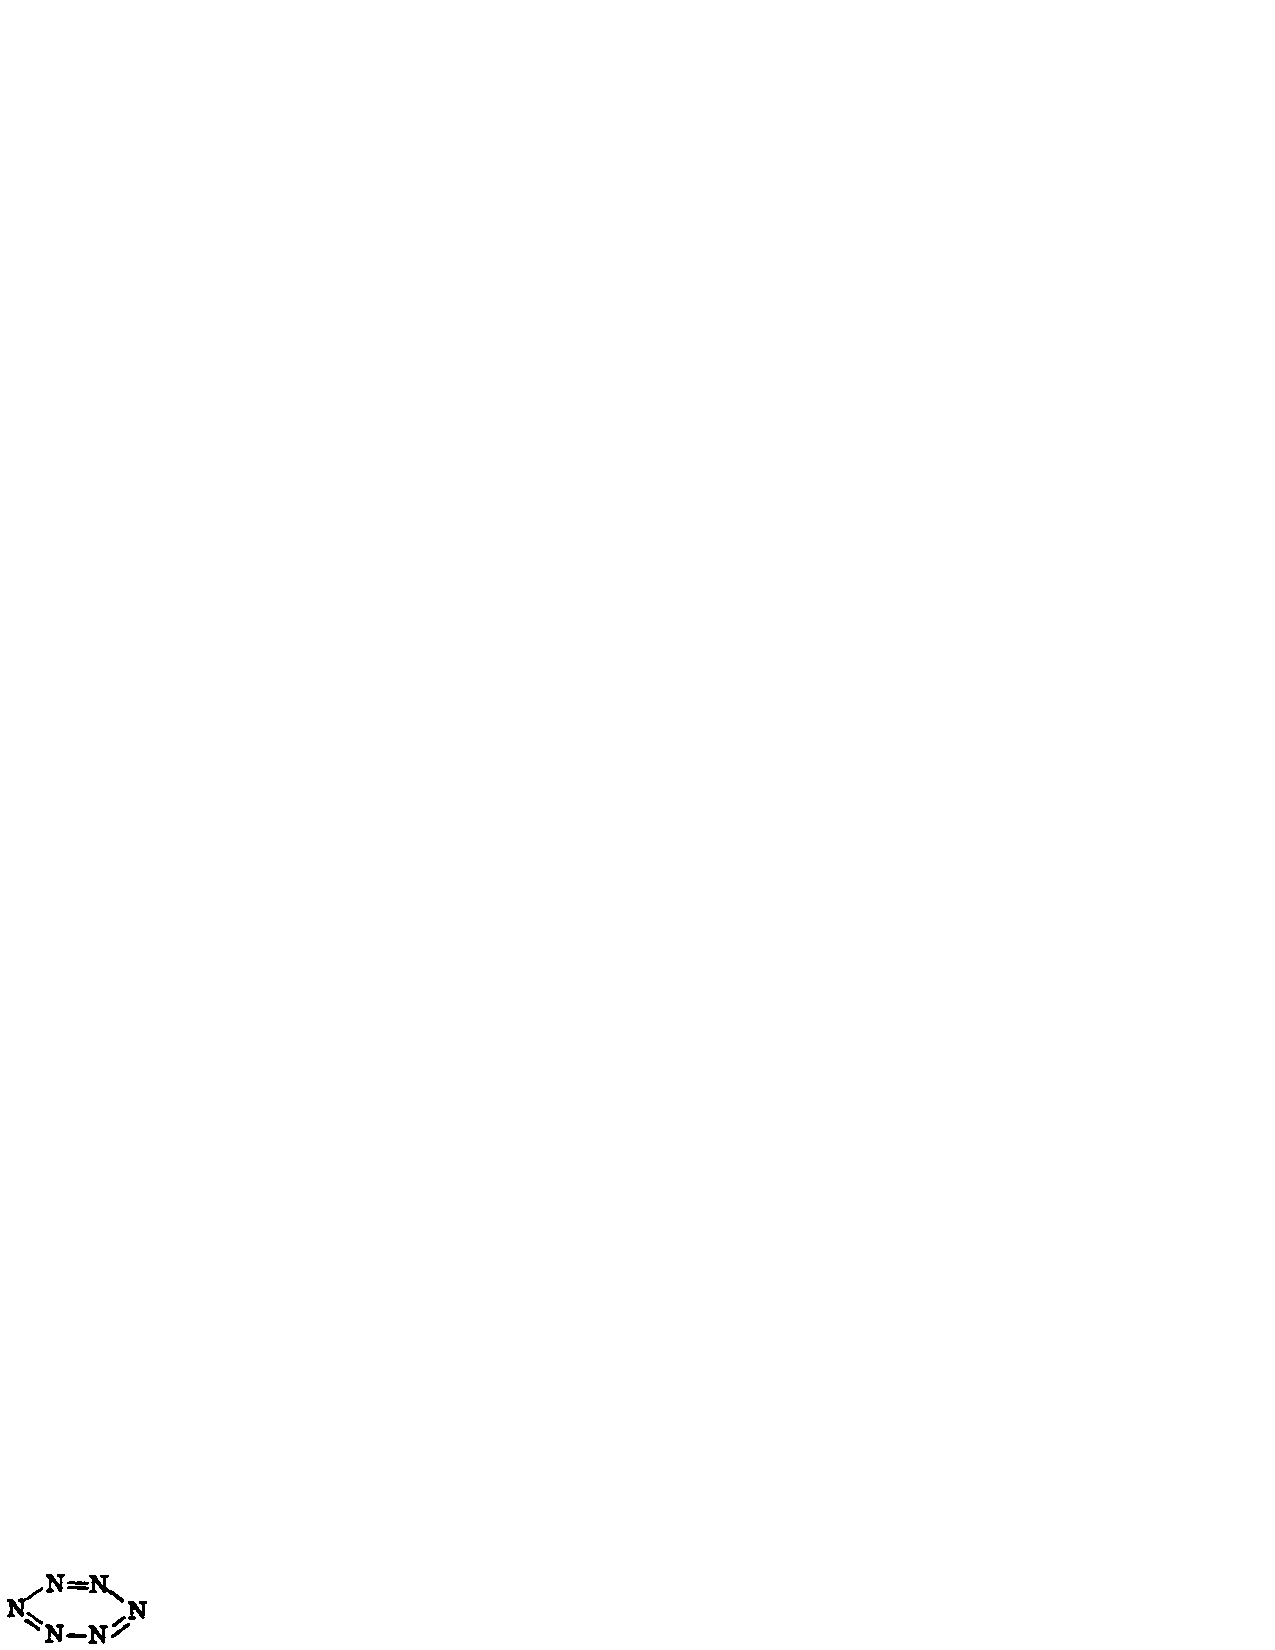
\includegraphics{fg12-06}
\end{equation}
With six sigma bonds and three pi bonds this should have a cohesive energy of
$\sim 6 * 55 + 3/1 * (225 - 55) = 585$ kcal, which would be 90 kcal above 
that of the N$_2$ molecules.  Such a species has not been observed.

A species which is observed is the azide radical N$_3$, a linear molecule with 
equal bond lengths, 1.1815 \AA.  Starting with $p^3$ configurations on each 
N would lead to
\begin{equation}
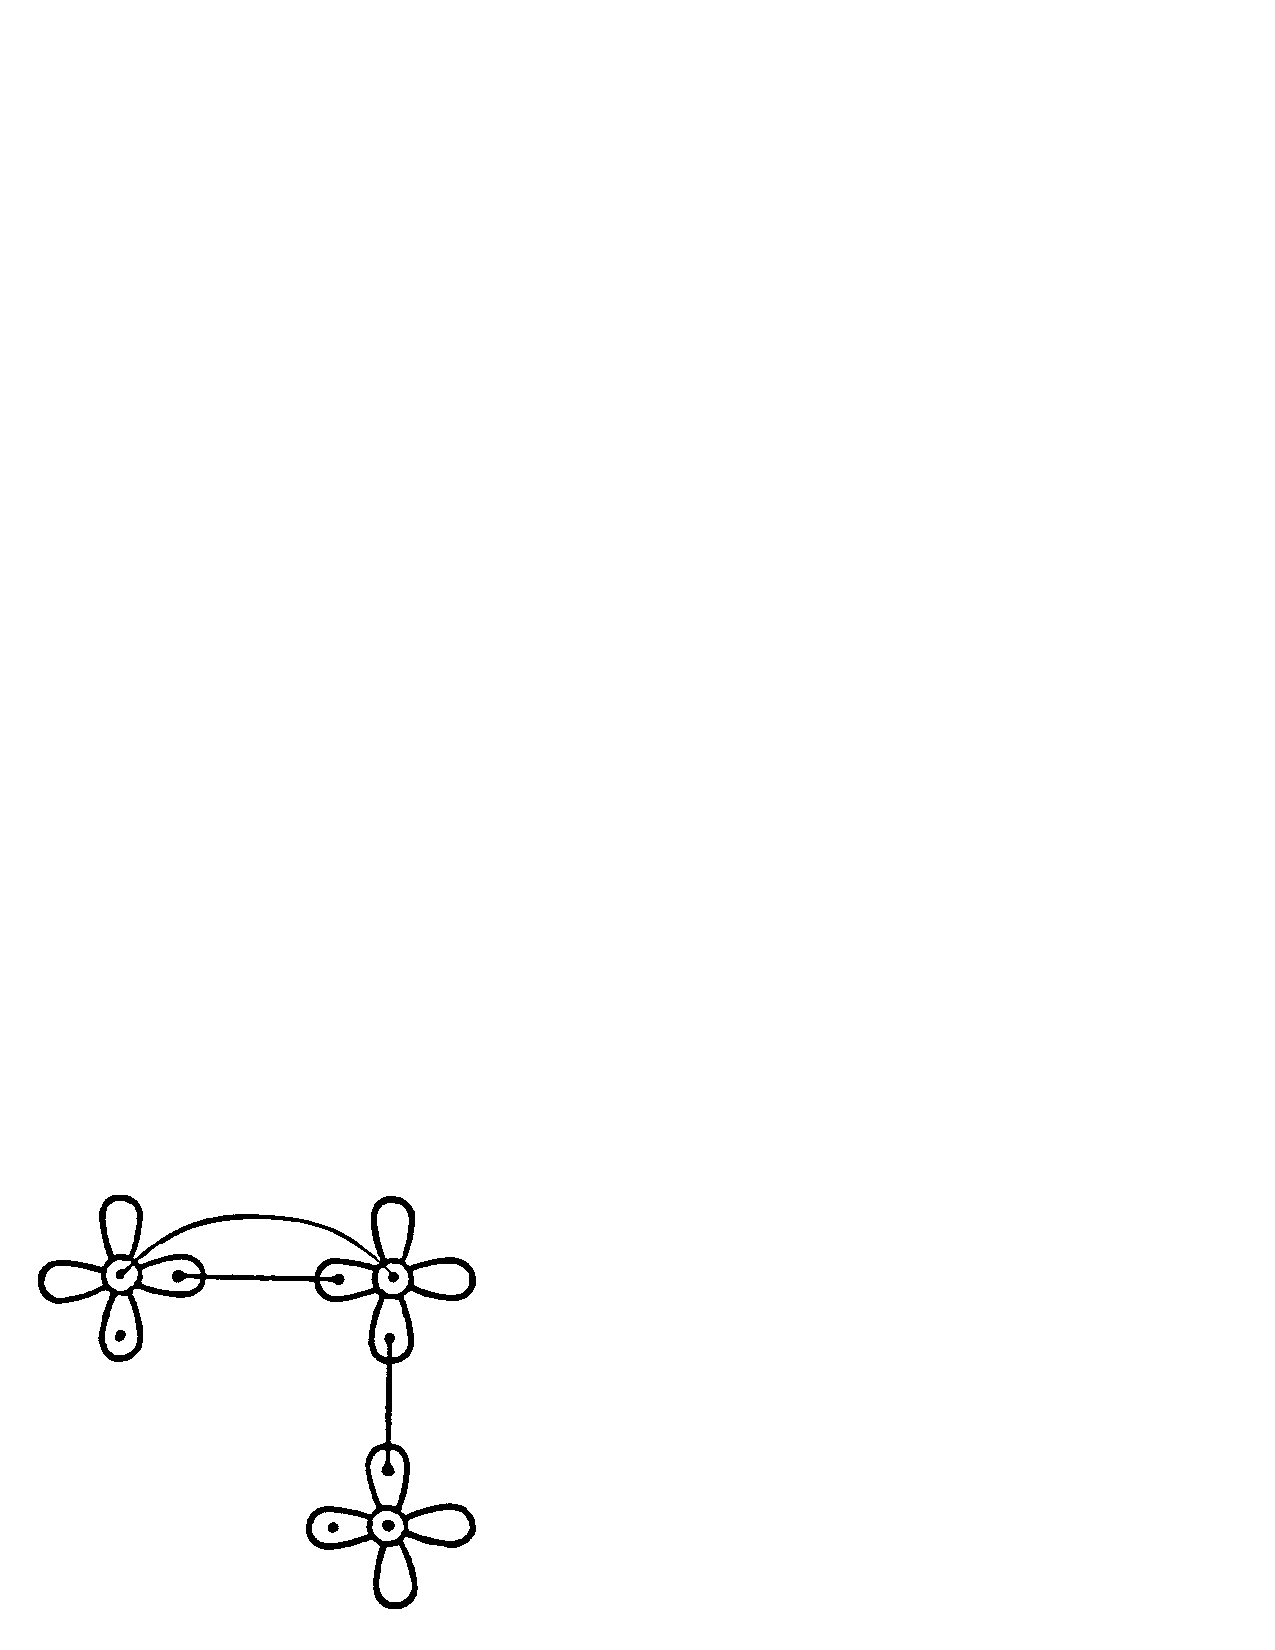
\includegraphics{fg12-07}
\end{equation}
which could close leading to a cyclic structure of the form
\begin{equation}
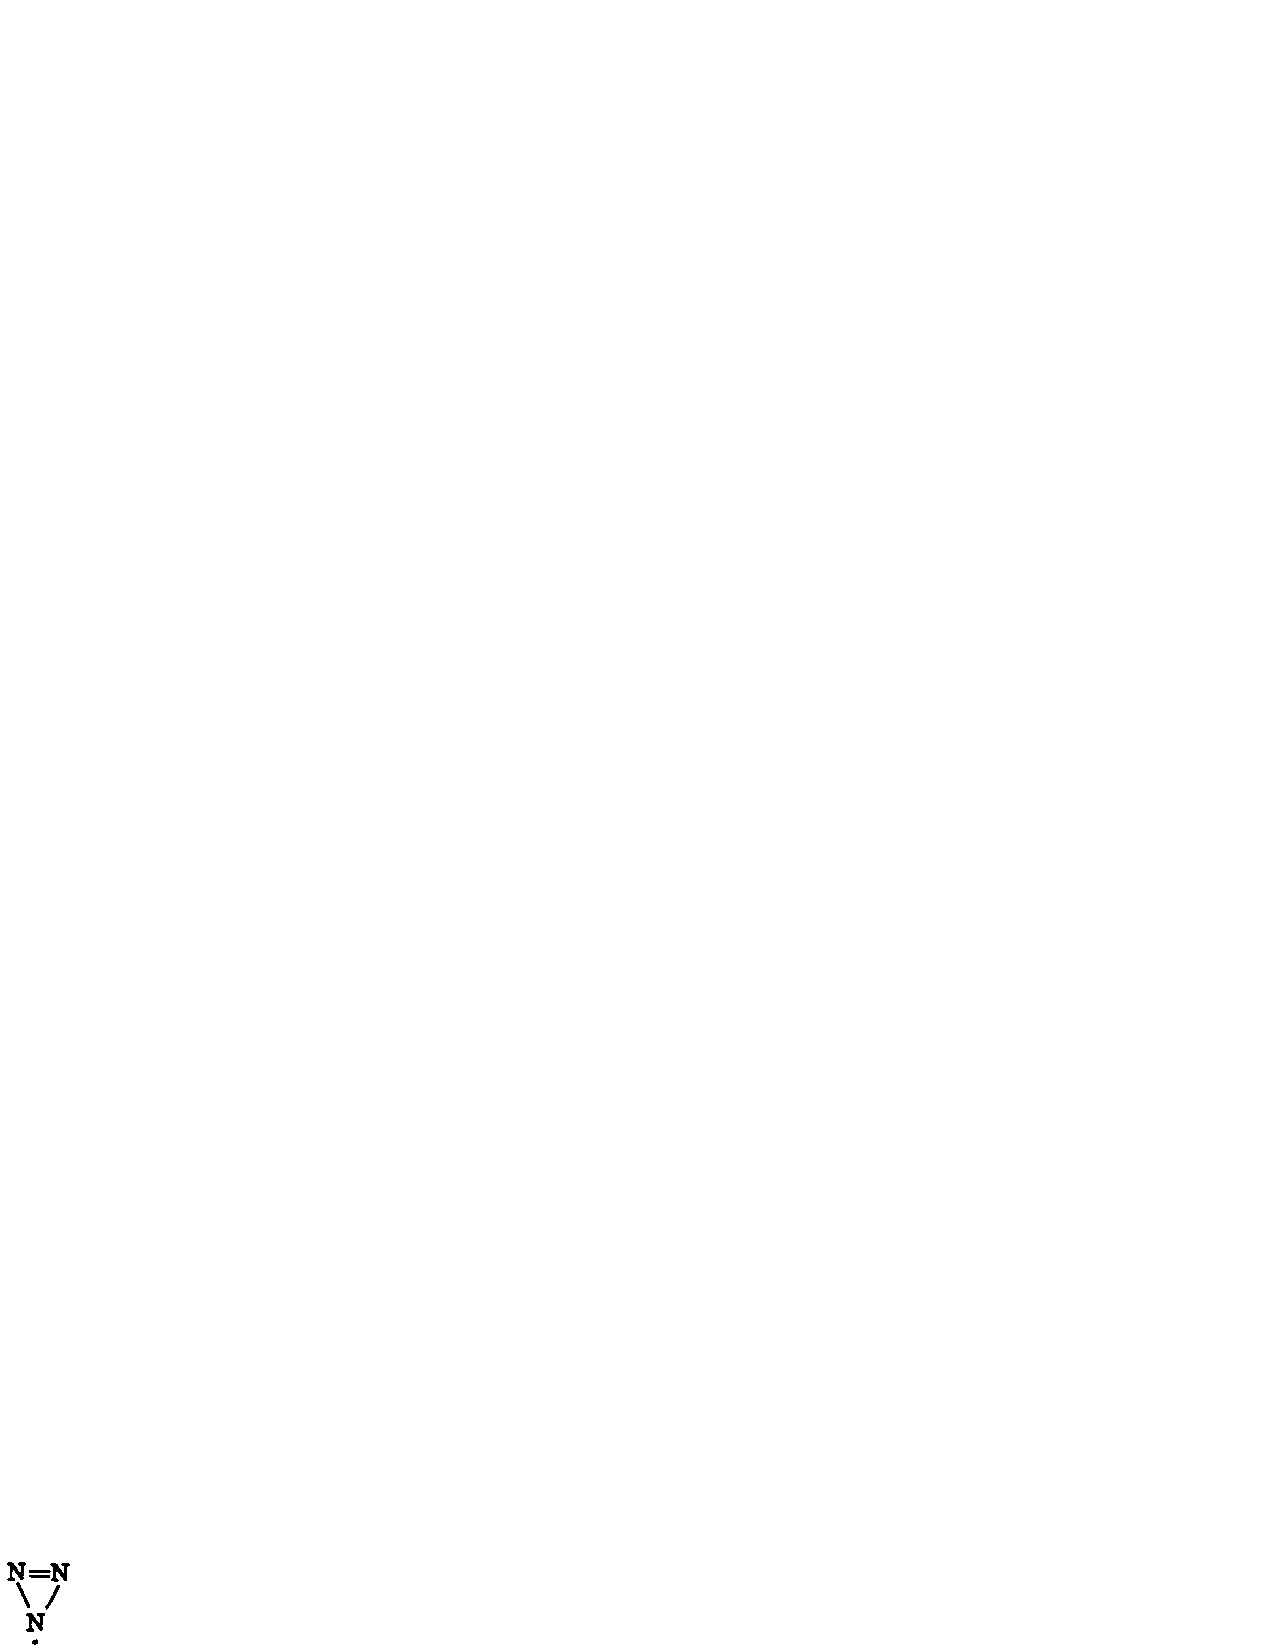
\includegraphics{fg12-08}
\end{equation}
How do we construct the configuration for linear N$_3$ molecule?  
Consider, for a moment, that one N atom is ionized leading to
\begin{equation}
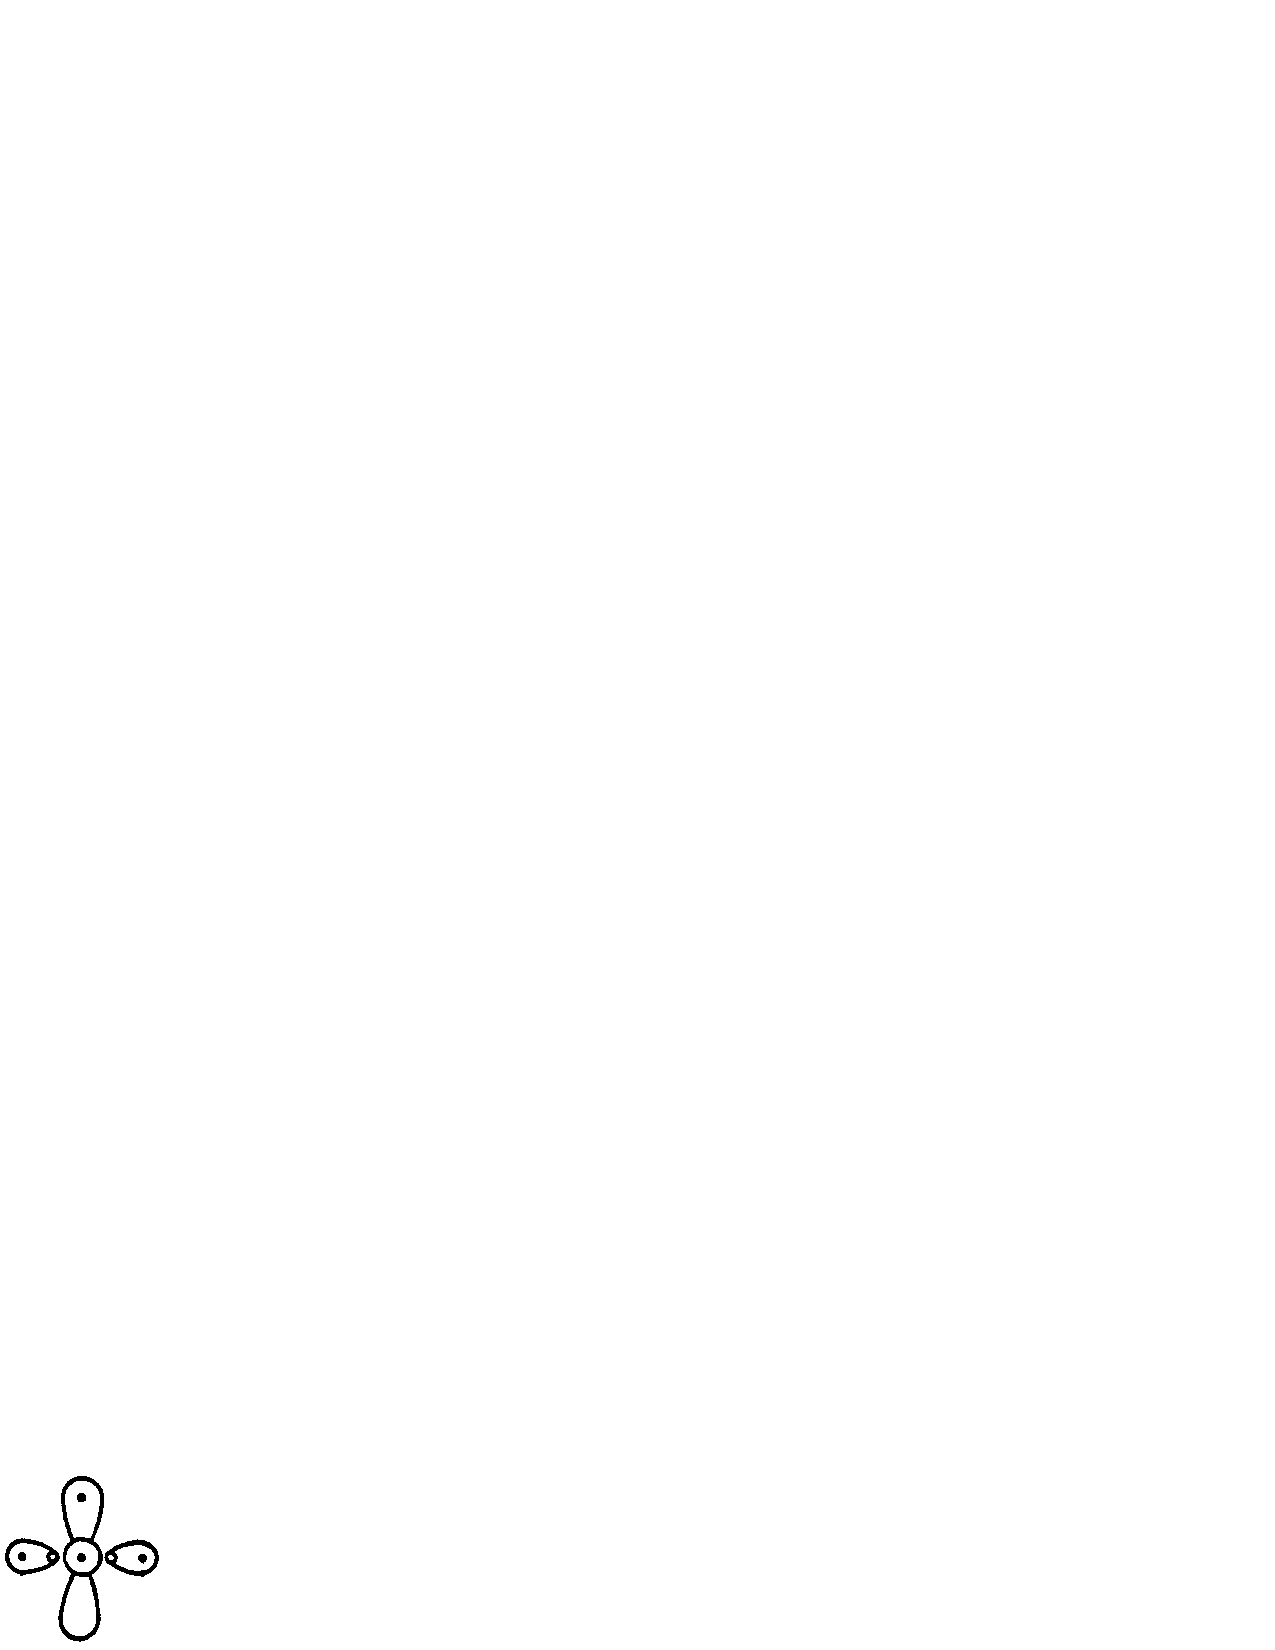
\includegraphics{fg12-09}
\end{equation}
A ground state N atom, $p^3$, can then be bonded to each side leading to
\begin{equation}
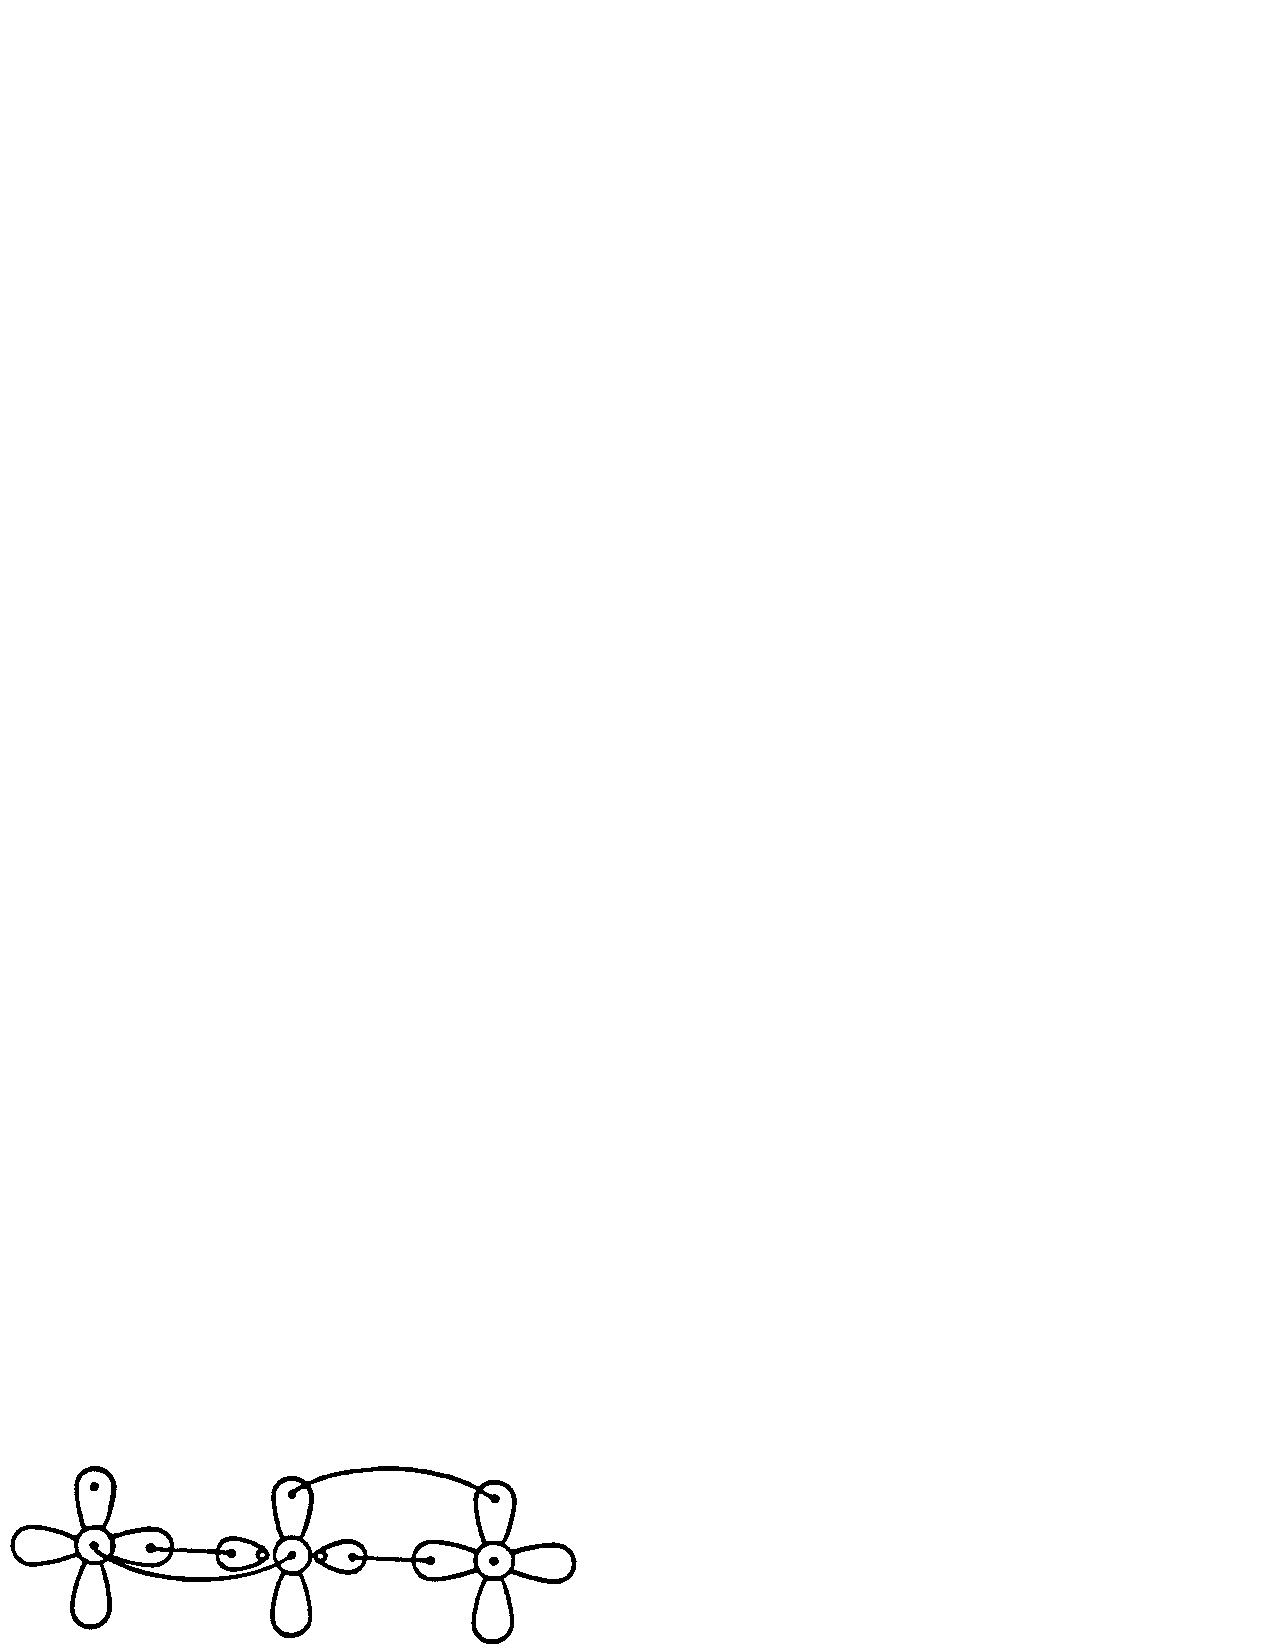
\includegraphics{fg12-10}
\end{equation}
and putting the electron back onto a terminal atom leads to
\begin{equation}
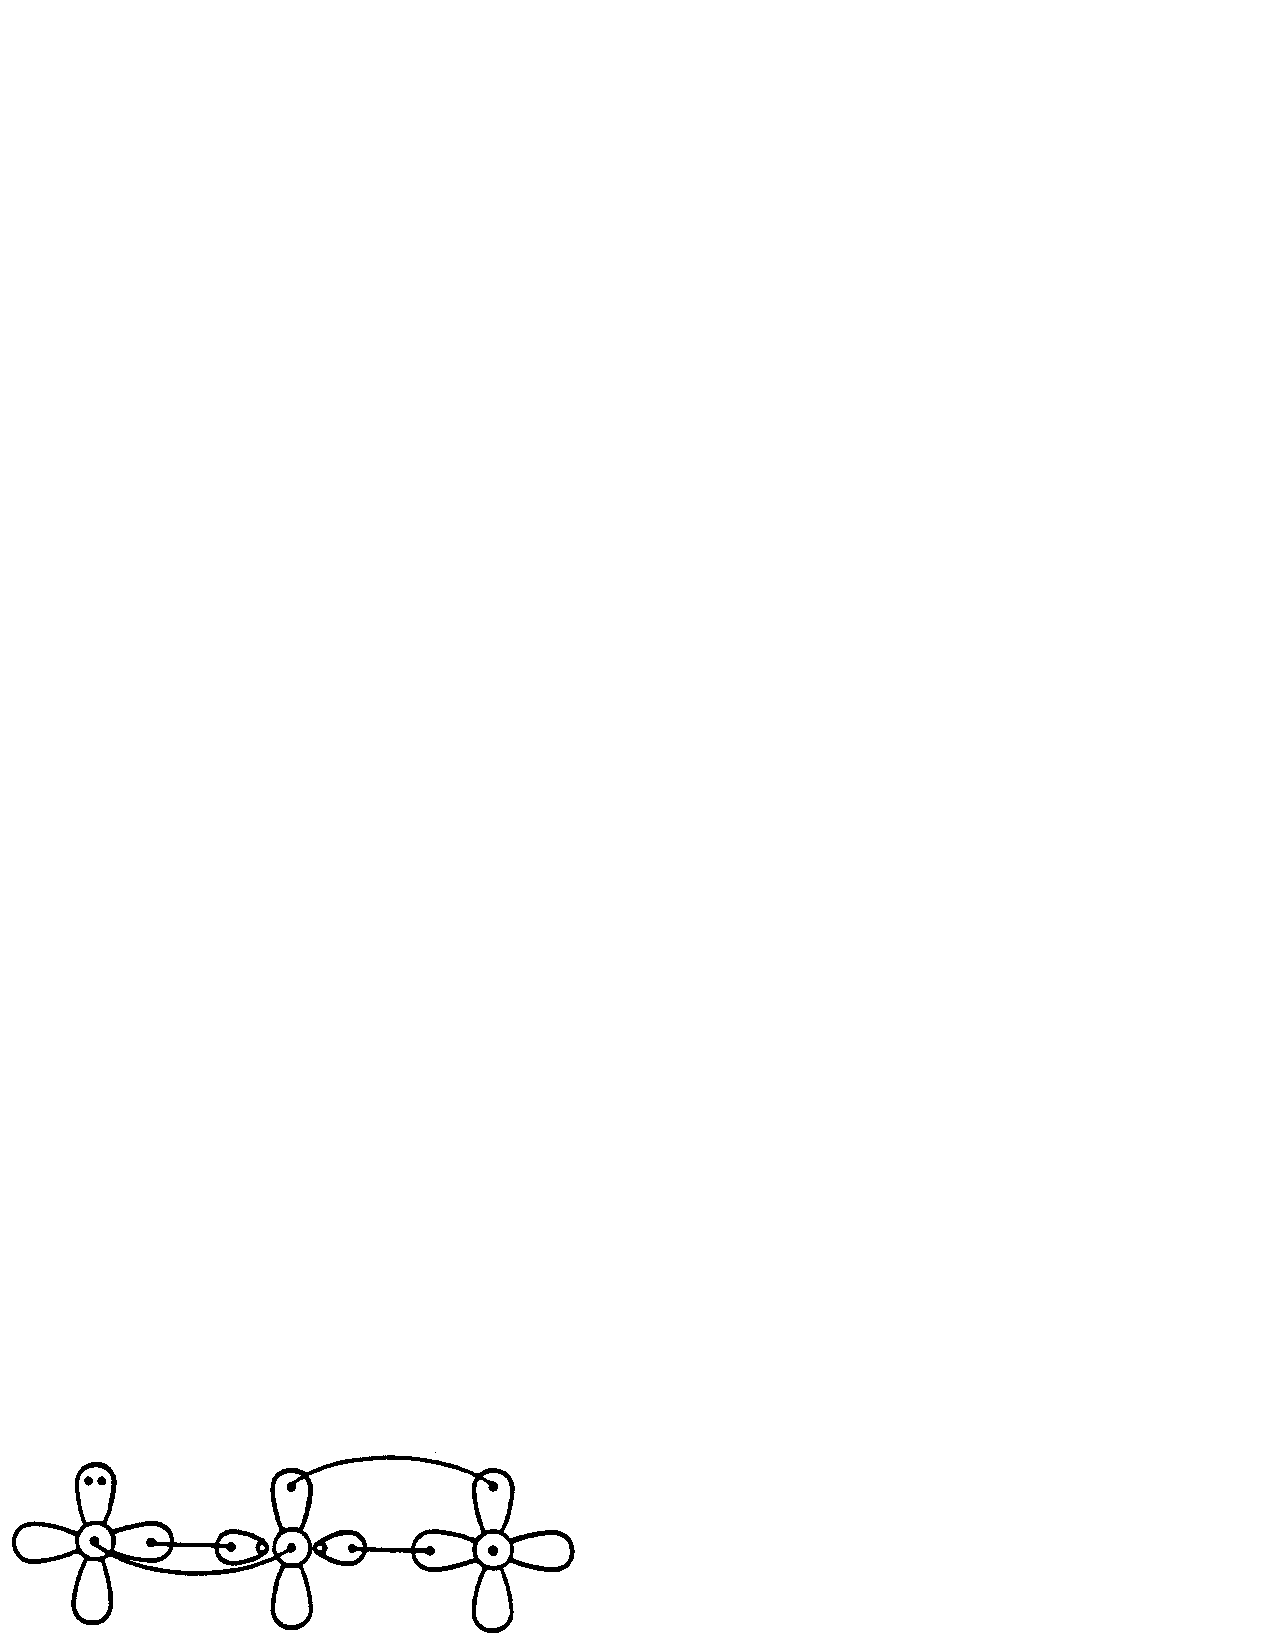
\includegraphics{fg12-11}
\end{equation}
which can resonate with
\begin{equation}
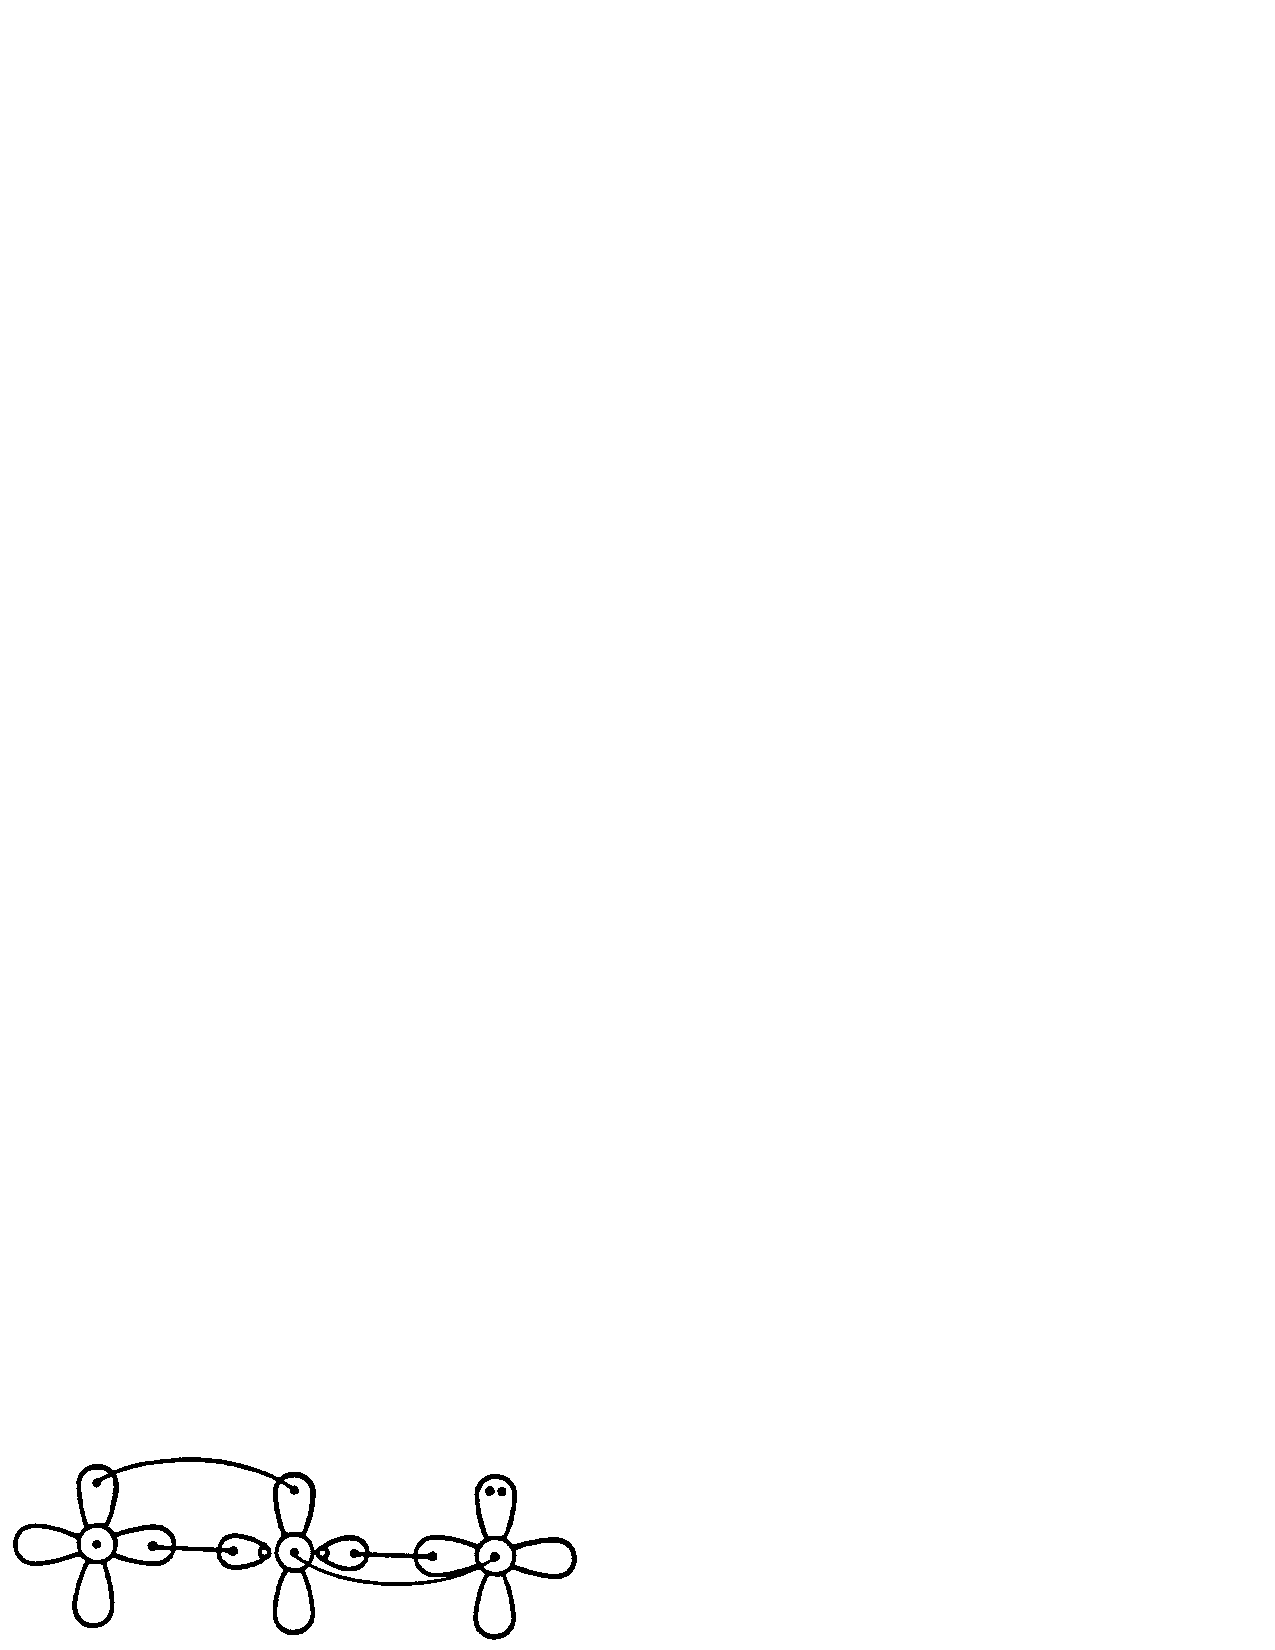
\includegraphics{fg12-12}
\end{equation}
leading to a ${^2\Pi}_g$ state.  This $N_3$ molecule is stable by 12.8 kcal with 
respect to N$_2 +$ N but two such
N$_3$ molecules are unstable with respect to three N$_2$ molecules by 199.4 
kcal.  Even so, it is
possible to make N$_3$ molecules.  Please don't do this near my office.

The total cohesive energy of N$_3$ is 237.8 kcal.  If one assumed that 
each sigma bond is worth 55 kcal and
each pi bond is worth 85 kcal, then the energy of N$_3$ is 42 kcal higher than 
expected, which could
be considered as the cost of transferring the electron from the center to 
terminal N.

Bonding an H to N$_3$ leads to
\begin{equation}
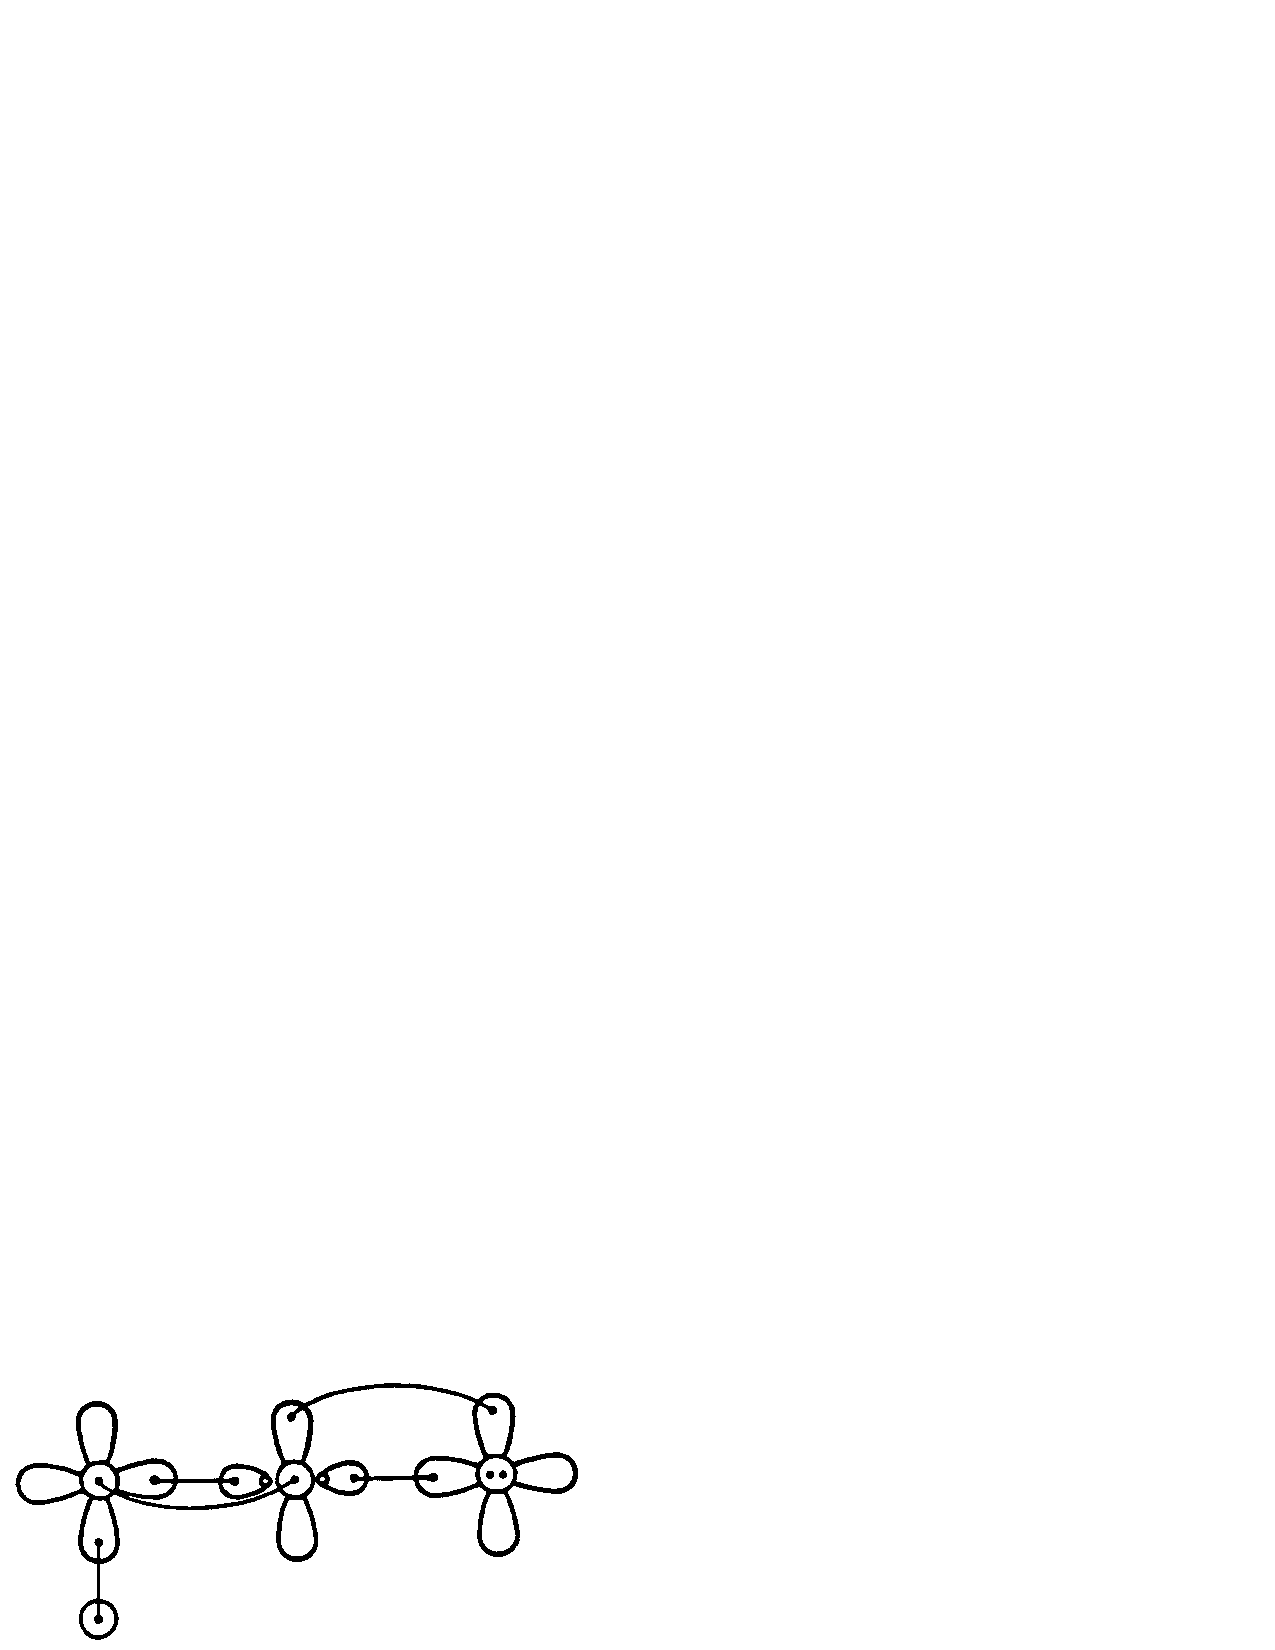
\includegraphics{fg12-13}
\end{equation}
Thus, the internal NN bond, 1.237 \AA, has a bond length comparable to a 
normal NN double bond, e.g.,
1.252 \AA\ for trans HN = NH.  However, the external NN bond is 
shorter, 1.133 \AA.    Comparing with
the bond length in N$_2$, 1.098 \AA, and N$^+_2$, 1.116 \AA, 
it is as if the external NN bond were of order 2-1/2, as in N$^+_2$.  
This suggests incorporation of
\begin{equation}
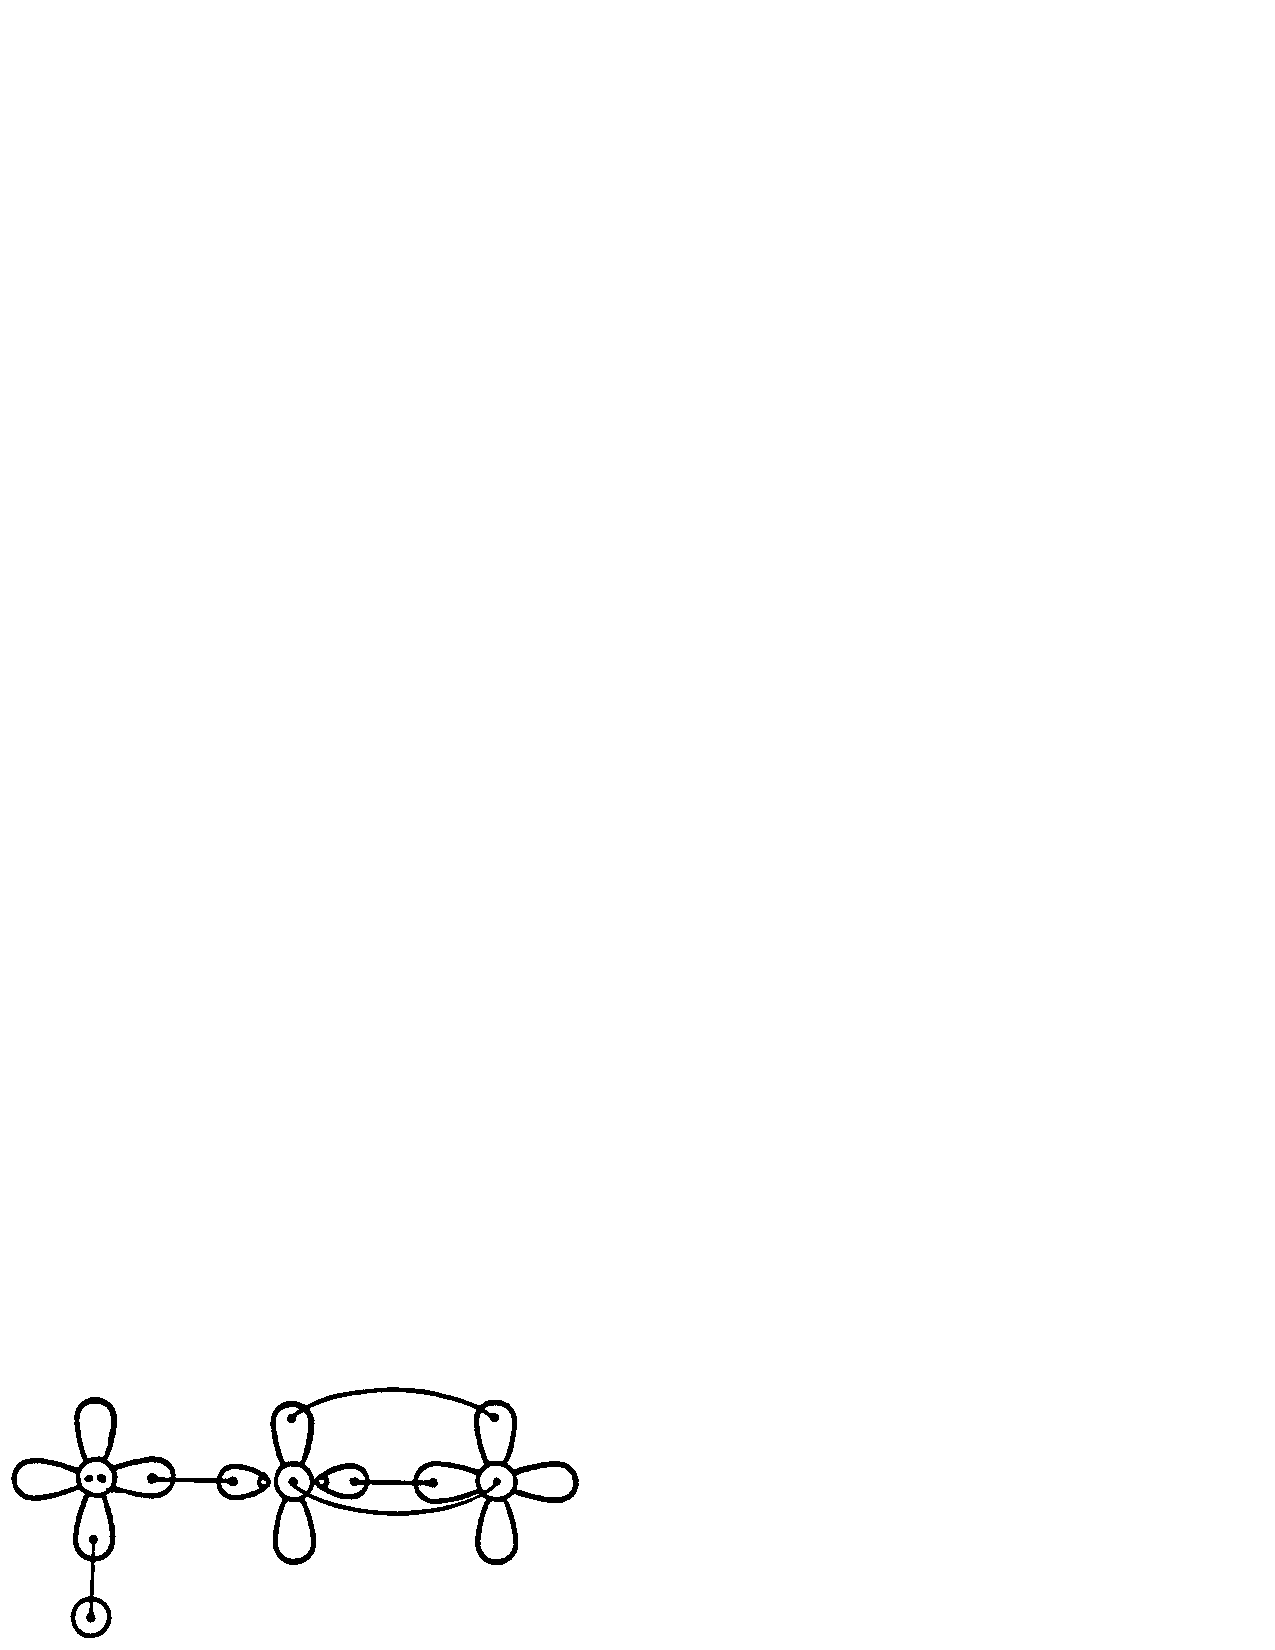
\includegraphics{fg12-14}
\end{equation}
character into the wavefunction.

\subsection{Bond Lengths}

\begin{table}
\caption{Properties of crystals in the N column.$^a$}
\label{chap12-tab4}
\begin{tabular}{ccccccc}\\ \hline
& &\multicolumn{2}{c}{Cohesive 
Energy$^a$}&$T_{mp}$$^b$&$\Delta$H$_m$$^b$&$T_{bp}$$^b$\cr
& &\multicolumn{2}{c}{298 K} &K&Kcal&$^{\circ}$K\cr
& &Ref. 1 & Ref.2\cr

P &	black, orthorhombic & 84.60\cr
& red, triclinic, cubic & 79.40	 & 79.78 & & 704\cr
& $\alpha$-white, cubic & 75.20 & 75.62 & 317.3$^d$ & 550$^f$\cr
& amorphous, red & 77.0\cr
As & $\alpha$, rhombohedral, & 72.3 & 72.12 & (1081)$^c$ & & 
876$^e$\cr
& ~~~~ gray, metallic\cr
& $\gamma$, yellow, cubic & 68.8\cr
& amorphous orthorhombic & 71.3\cr
Sb & II, rhombohedral, & 62.7 & 63.23 & 904 & 4.75 & 1860\cr
& metallic \cr
& IV, amorphous & 60.16\cr
Bi & rhombohedral metallic & 49.5 & 50.1 & 544.52 & 2.7 & 1837\cr
\hline
\end{tabular}\\
$^a$ Reference la.
$^b$ Based on reference 2, unless indicated otherwise. 
$^c$ For a pressure of one atmosphere, As sublimes without 
melting at 870 K.  This value is extrapolated from high-pressure 
studies. 
$^d$ Converts to $\beta$-white P below 195.4 K.
$^e$ $\Delta H_{v,298} = 9.15$ kcal to yield one-fourth As$_4$.
$^f$ $\Delta H_{v,298} = 3.52$ kcal to yield one-fourth P$_4$.
\end{table}

\begin{table}
\caption{Bond lengths for the N column.}
\label{chap12-tab5}
\begin{tabular}{cccccc}\\ \hline
&\multicolumn{2}{c}{$M-M$}&$M=M$ & $M \equiv M^b$&Effect of Two\cr
& Solid$^a$ & Molecule$^d$ & & & pi Bonds\cr

N & - & 1.45$^e$ & 1.23$^{d,h}$ & 1.10 & $-$0.35\cr
P & 2.234 & 2.23$^f$ & & 1.89 & $-$0.32\cr
As & 2.517 & 2.435$^g$ & & 2.10 & $-$0.34\cr
Sb & 2.908 & (2.83)$^c$ & & 2.34 & ($-$0.49)\cr
Bi & 3.072 & (2.99)$^c$ & & 2.66 & ($-$0.33)\cr
\hline
\end{tabular}\\
$^a$ Table 18b.
$^b$ Table 15.
$^c$ Assuming a decrease of 0.08 \AA\ from solid to molecule, as found for
As.
$^d$ Reference 7.
$^e$ Using 1.447 for H$_2$N$-$NH$_2$, and 1.457 for 
(SiH$_3$)$_2$N$-$N(SiH$_3$)$_2$. Ignore 1.492 for F$_2$N$-$NF$_2$,
1.427 for  H$_2$N$-$NO$_2$, 1.782 for O$_2$N$-$NO$_2$, and 1.864 for
ON$-$NO$_2$. 
$^f$ 2.219 for $H_2P-PH_2$, 2.218 for $H_2P-PF_2$, and 2.21 
for $P_4S_3$.  Ignore 2.281 for $F_2P-PF_2$.
$^g$ Based on As$_4$.
$^a$ Using 1.252 for trans-HN=NH, 1.214 for cis-FN=NF, and 1.231 for 
trans-FN=NF.
\end{table}

Bond lengths for various species are summarized in Table
\ref{chap12-tab5}.  For N, P, and As there is a consistent decrease of
$\sim$0.34 \AA\ upon going from a single bond to a triple bond.  For
$N_2$, the length of a double bond is $\sim$1.23 \AA\ which is 63
percent of the way from a single bond and a triple bond.  This trend
compares well with that of the corresponding series in C
\begin{tabular}{ccccc}\\
\multicolumn{2}{c}{C species}& \multicolumn{2}{c}{N species}& Difference\\
\chem{HC\equiv CH} & 1.205 & \chem{N\equiv N} & 1.098 & 0.107 \\
\chem{H_2C=CH_2} & 1.336 & \chem{HN=NH} & 1.252 & 0.084 \\
\chem{H_3C-CH_3} & 1.536 & \chem{N_2N-NH_2} & 1.447 & 0.089 
\end{tabular}

One very odd result is that H$_2$N $-$ PF$_2$ has an NP
bond length of 1.650 \AA\ which is considerable below the average, 
1.83 \AA, of $N-N$ and $P-P$, and is approximately the value expected 
for a double bond $N=P$.  The molecule
\begin{equation}
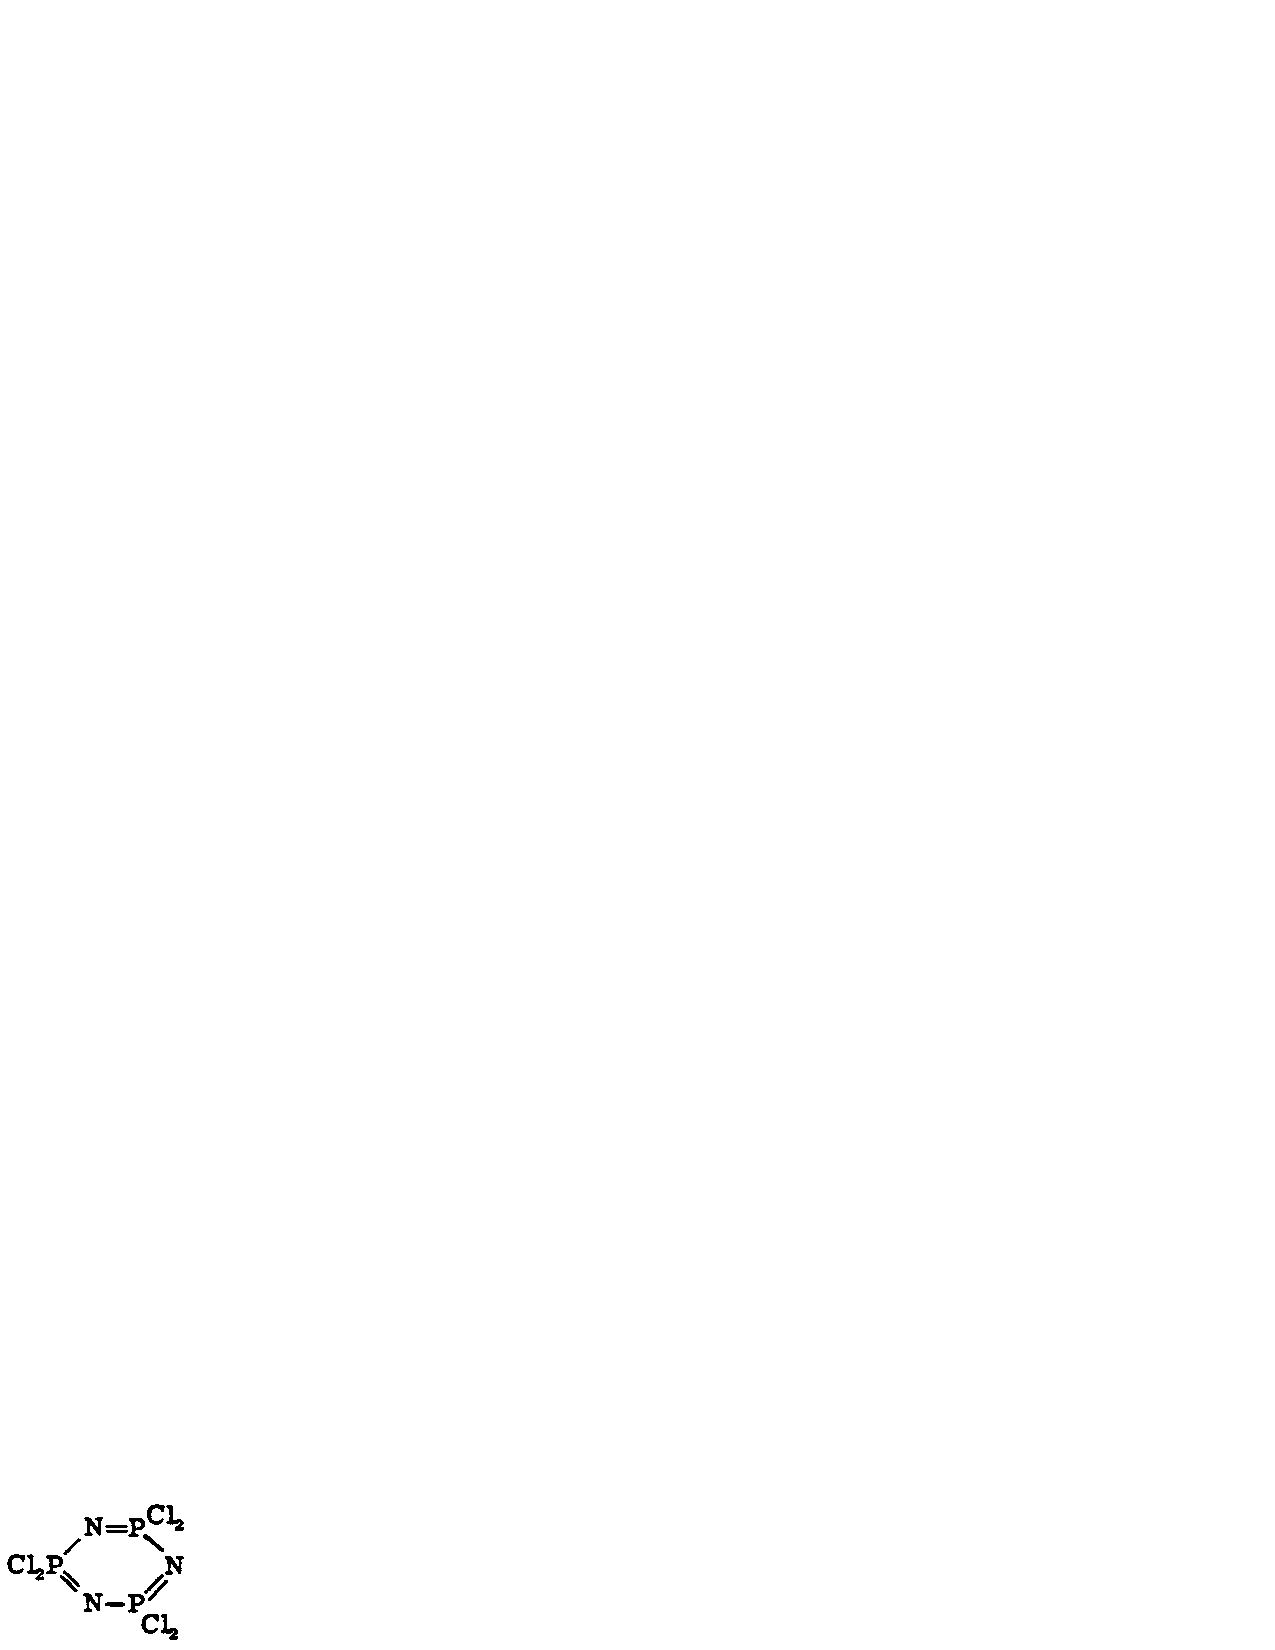
\includegraphics{fg12-15}
\end{equation}
is nearly planar and leads to equal NP bond lengths of 1.582 \AA.  This can be 
considered as the bond length for bond order 1-1/2. However, to do so we must
use all five valence electrons of P to make five different bonds.  
PF$_5$ can do this, an issue we take up later.

\section{The Oxygen Column}

The vapor over condensed phases of S and Se, and perhaps Te, contain cyclic 
six- and eight-membered rings and under certain conditions other cyclic 
species.  Thus, Se$_6$ is observed to have the chair conformation geometry
\begin{equation}
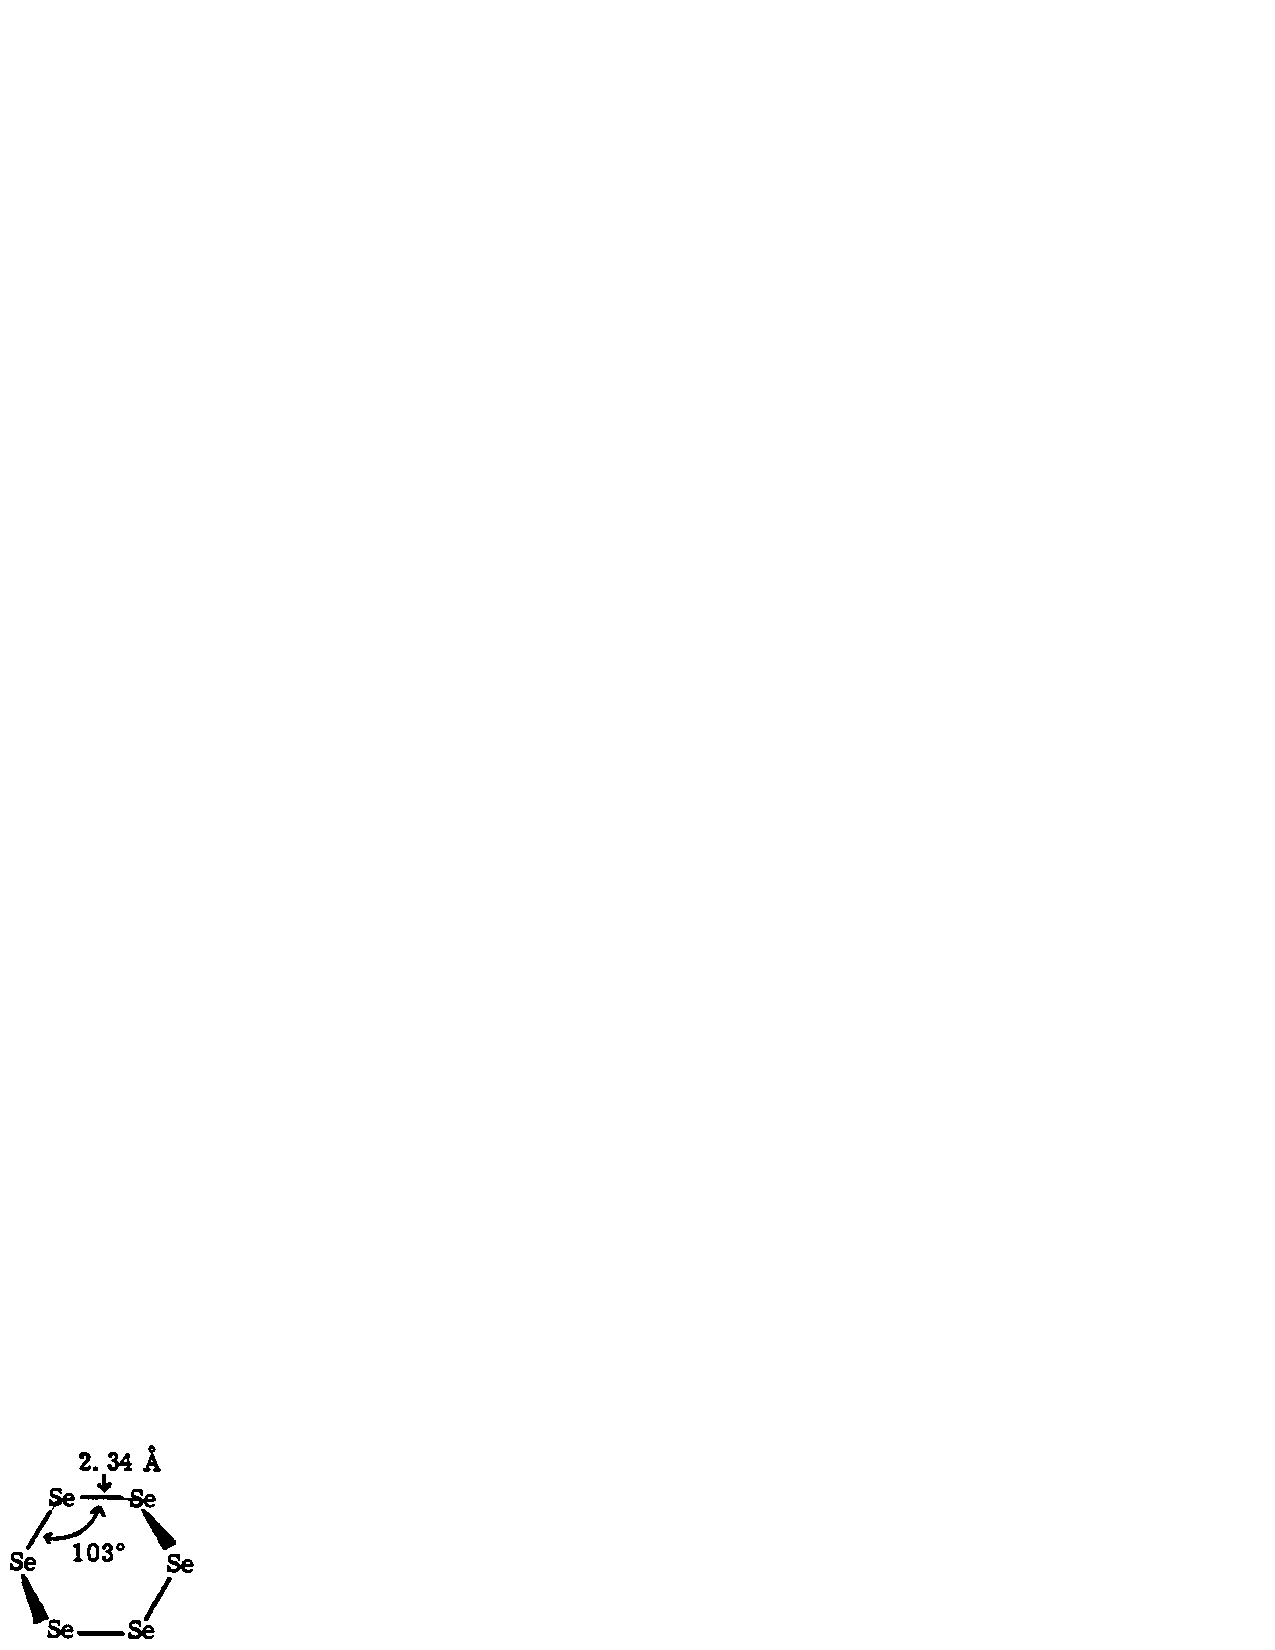
\includegraphics{fg12-16}
\end{equation}

These rings involve two bonds to each atom and hence are expected to be 
strongly bound species.  For Te and Se the stable crystals exhibit infinite 
chains having a similar bonding, whereas Po is a metal with six covalent 
bonds to each atom.  For S the stable crystal structure consists of cyclic 
S$_8$ molecules weakly bonded to each other.  On the other hand, 
O$_2$2 crystallizes as a molecular solid with only weak interaction 
between the O$_2$ molecules, and the only longer polymer of oxygen is ozone, a
reactive unstable molecule.

As will be discussed below, the origin of this difference is that S, Se, 
and Te lead to pi bonds significantly weaker than the sigma bonds, whereas 
O$_2$ leads to pi bonds considerably stronger than the sigma
bonds.  First we will consider the case of sulfur.

\subsection{Sigma Versus Pi Bonds}

\subsubsection{Singly Bonded Sulfur Atoms}

\begin{table}
\caption{S-S bond energies.  All energies in kcal and 
evaluated at 298$^{\circ}$K.}
\label{chap12-tab6}
\begin{tabular}{ccccc}\\ \hline
& & Energy &\multicolumn{2}{c}{Bond Energies}\cr
& $\Delta$H$_f$(H$_2$S$_n$)$^a$ & Change & Average & Incremental\cr

HS-SH $\rightarrow$2HS & 2.53 & 65.7 & 65.7 & 65.7\cr
HS-S-SH $\rightarrow$ 2HS+S & 3.59 & 131.2 & 65.6 & 65.6\cr
HS-S-S-SH $\rightarrow$ 2HS + 2S & 5.71 & 195.7 & 65.2 & (65.6) 
64.5\cr
HS-S-S-S-SH $\rightarrow$ 2HS + 3S & 7.98 & 260.0 & 65.0 & (65.6) 
64.4\cr
\hline
\end{tabular}\\
$^a$Reference 1, $\Delta$H$_f$(HS) = 34.10, $\Delta$H$_f$(S) = 66.636.
\end{table}

Consider the series of bond energies in Table \ref{chap12-tab6}. The
conclusion is that the average S-S bond strength is fairly independent
of whether an H or an S is bonded to the S, the results being
\begin{tabular}{cc}\\
Species & E (kcal/mol) \\
\chem{HS-SH} & 65.7 \\
\chem{SS-SH} & 65.6 \\
\chem{SS-SS} & 64.4 
\end{tabular}
Now consider the average bond energies of the cyclic sulfur molecules,
as given in Table \ref{chap12-tab7}.

\begin{table}
\caption{Bond energies in kcal, of cyclic molecules, 
evaluated at 298$^{\circ}$K.}
\label{chap12-tab7}
\begin{tabular}{ccc}\\ \hline

& $\Delta$H$_f^a$ & Average Bond Energy\cr

S$_4$ &32.7 & 58.5\cr
S$_6$ & 24.5 & 62.6\cr
S$_8$ & 25.45 & 63.58\cr
\hline
\end{tabular}\\
$^a$Reference 1, $\Delta$H$_f$(S) = 66.636.
\end{table}

Since S$_2$ has the singly occupied orbitals in opposite planes,
\begin{equation}
% missing figure chap12 p 15
%\includegraphics{fg12-}
\end{equation}
we expect that S$_n$ polymers would prefer dihedral angles near 
90$^{\circ}$.  For small molecules this is not possible, leading 
to weaker bond energies because of strain, as observed. The largest 
species, S$_8$, probably has little strain and leads to a single bond 
energy, 63.6 kcal, close to the value, 64.4 kcal, obtained for
HS$_n$H. Thus, we will adopt 64.0 kcal as the average single bond 
energy of sulfur.

The bond energy of S$_2$ is 102.6 kcal, suggesting that the pi bonding is 
worth 38.6 kcal.  Since the pi bond is so much weaker than the sigma bond, 
it is easy to understand why S tends to form cyclic polymers.

\subsubsection{Singly Bonded Oxygen Atoms}

\begin{table}
\caption{O-O bond.}
\label{chap12-tab8}
\begin{tabular}{cccc}\\ \hline
& $\Delta$H$_{f298}$ & Energy & Length$^b$\cr
& (kcal)$^a$ & 298 K & \AA\cr

HO$-$OH & $-$32.53 & 51.51 & 1.465\cr
MeO$-$OH & & 48$^b$ & 1.466\cr
MeO$-$OMe & & 45$^b$ & 1.462\cr
\hline
\end{tabular}\\
$^a$$\Delta$H$_{f298}$(OH) = 9.49.
$^b$R. Bair, unpublished.
\end{table}

Consider the O-O bond energies in Table \ref{chap12-tab8}.  Based on
these results, we will consider an O-O single bond to be worth 48
kcal. Since the bond in O$_2$ is 118 kcal, this suggests that the pi
bonding in O$_2$ is worth 70 kcal.

Comparing with S, we find that the O-O sigma bond energy is 48 kcal, 
while the S-S is 64 kcal.  For pi bonds, oxygens are with 70 kcal, 
while surfurs are just 39 kcal.  Thus, ignoring strain
\begin{tabular}{cc}\\
Reaction & $\Delta$H (kcal/mol)\\
2\chem{O_2} $rightarrow$ 4-O ring & +44 kcal\\
3\chem{O_2} $rightarrow$ 6-O ring & +66 kcal
\end{tabular}
whereas, ignoring strain
\begin{tabular}{cc}\\
Reaction & $\Delta$H (kcal/mol)\\
2\chem{S_2} $rightarrow$ 4-S ring & -50 kcal\\
3\chem{S_2} $rightarrow$ 6-S ring & -75 kcal
\end{tabular}
Consequently, for oxygen, formation of cyclic polymers is very endothermic, 
whereas for S, Se, and Te formation of cyclic polymers is very exothermic,

Using these average bond energies we would expect cyclic ozone
to have a cohesive energy of (3 $\times$ 48) = 144 kcal, which would be 
bound by 26 kcal with respect to O$_2 +$ O.  Good quality 
calculations$^1$ show that the energy of cyclic ozone is 
approximately equal to that of O$_2$ + O
\begin{equation}
\chem{O_2} + O \rightarrow \chem{cyclic O_3} 
\end{equation}
has a $\Delta$H=4 kcal/mol, leading to a cohesive energy of 114 kcal.
L. B. Harding and W. A.  Goddard,$^1$ show that cyclic ozone is 28
kcal above the ground state of ozone. Since the cohesive energy of
ground state ozone is 118.0 + 24.2 = 142.2 kcal, we see that the
cohesive energy of cyclic ozone is 114 kcal.  Thus, we say that the
strain energy of (\ref{chap12-eqno5}) is 30 kcal.  For comparison, the
strain energy for cyclic \chem{CH_2} or epoxide is 26 kcal in both
cases.

\subsection{Bonding in Oxygen Containing Species}

\subsubsection{Perioxy Radicals}

Binding a monovalent atom, such as H, to O$_2$ leads from
(\ref{chap12-eqno2}) to
\begin{equation}
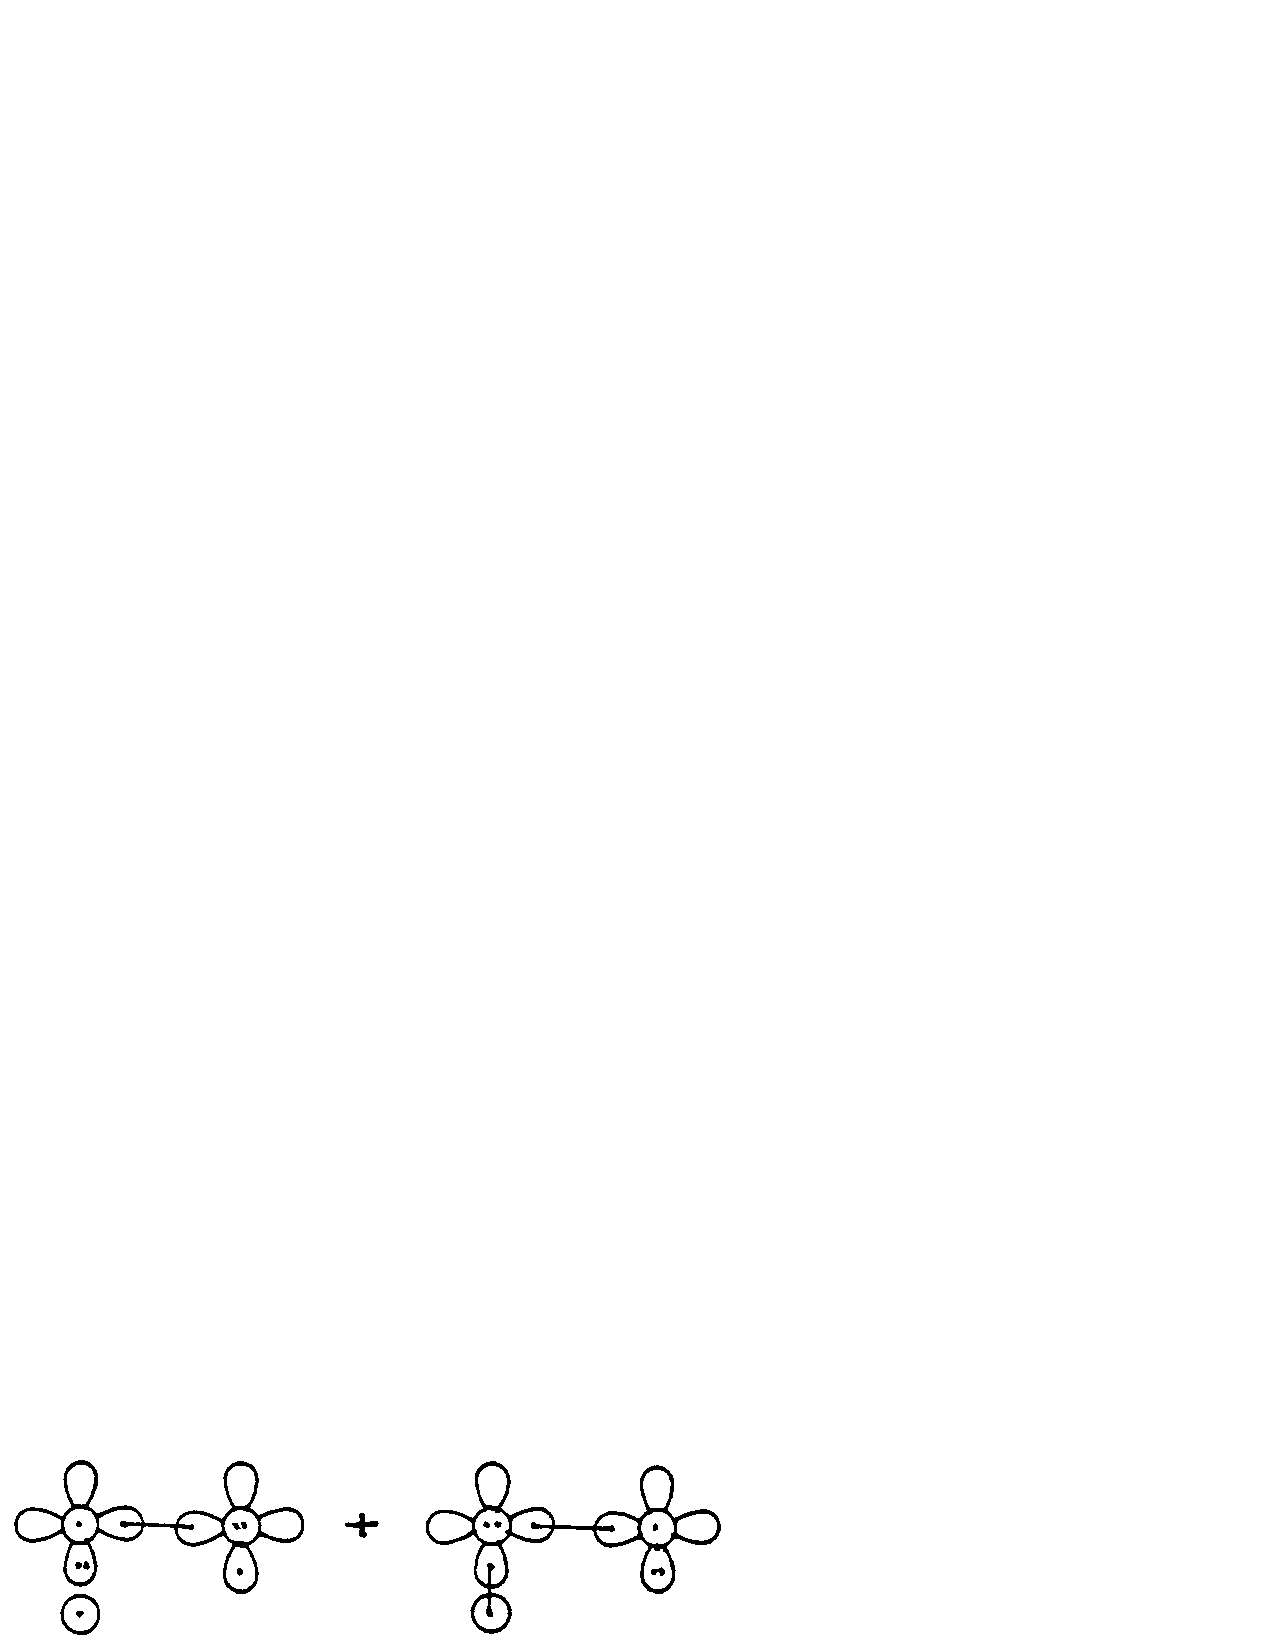
\includegraphics{fg12-17}
\label{chap12-eqno6}
\end{equation}
Note that only the right configuration makes a bond, leading to the 
single configuration
\begin{equation}
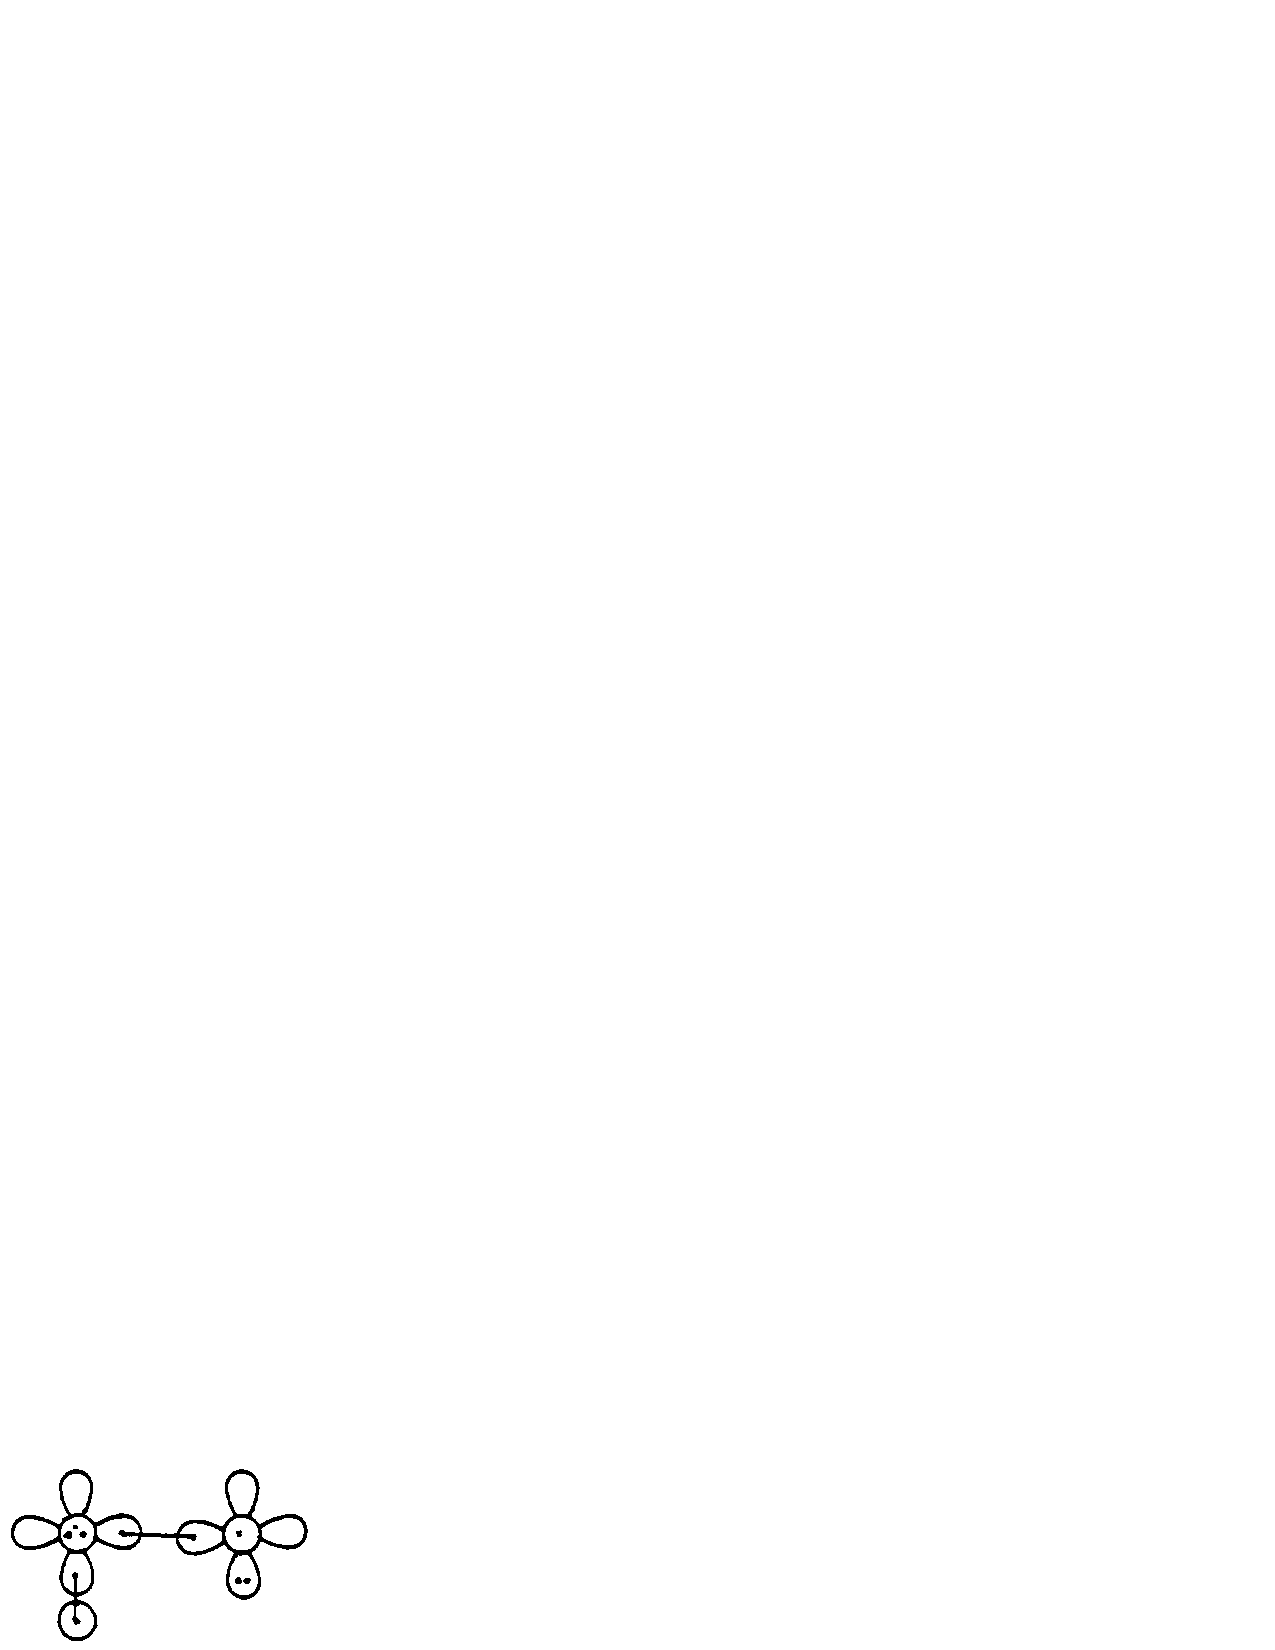
\includegraphics{fg12-18}
\label{chap12-eqno7}
\end{equation}
which we will often show as
\begin{equation}
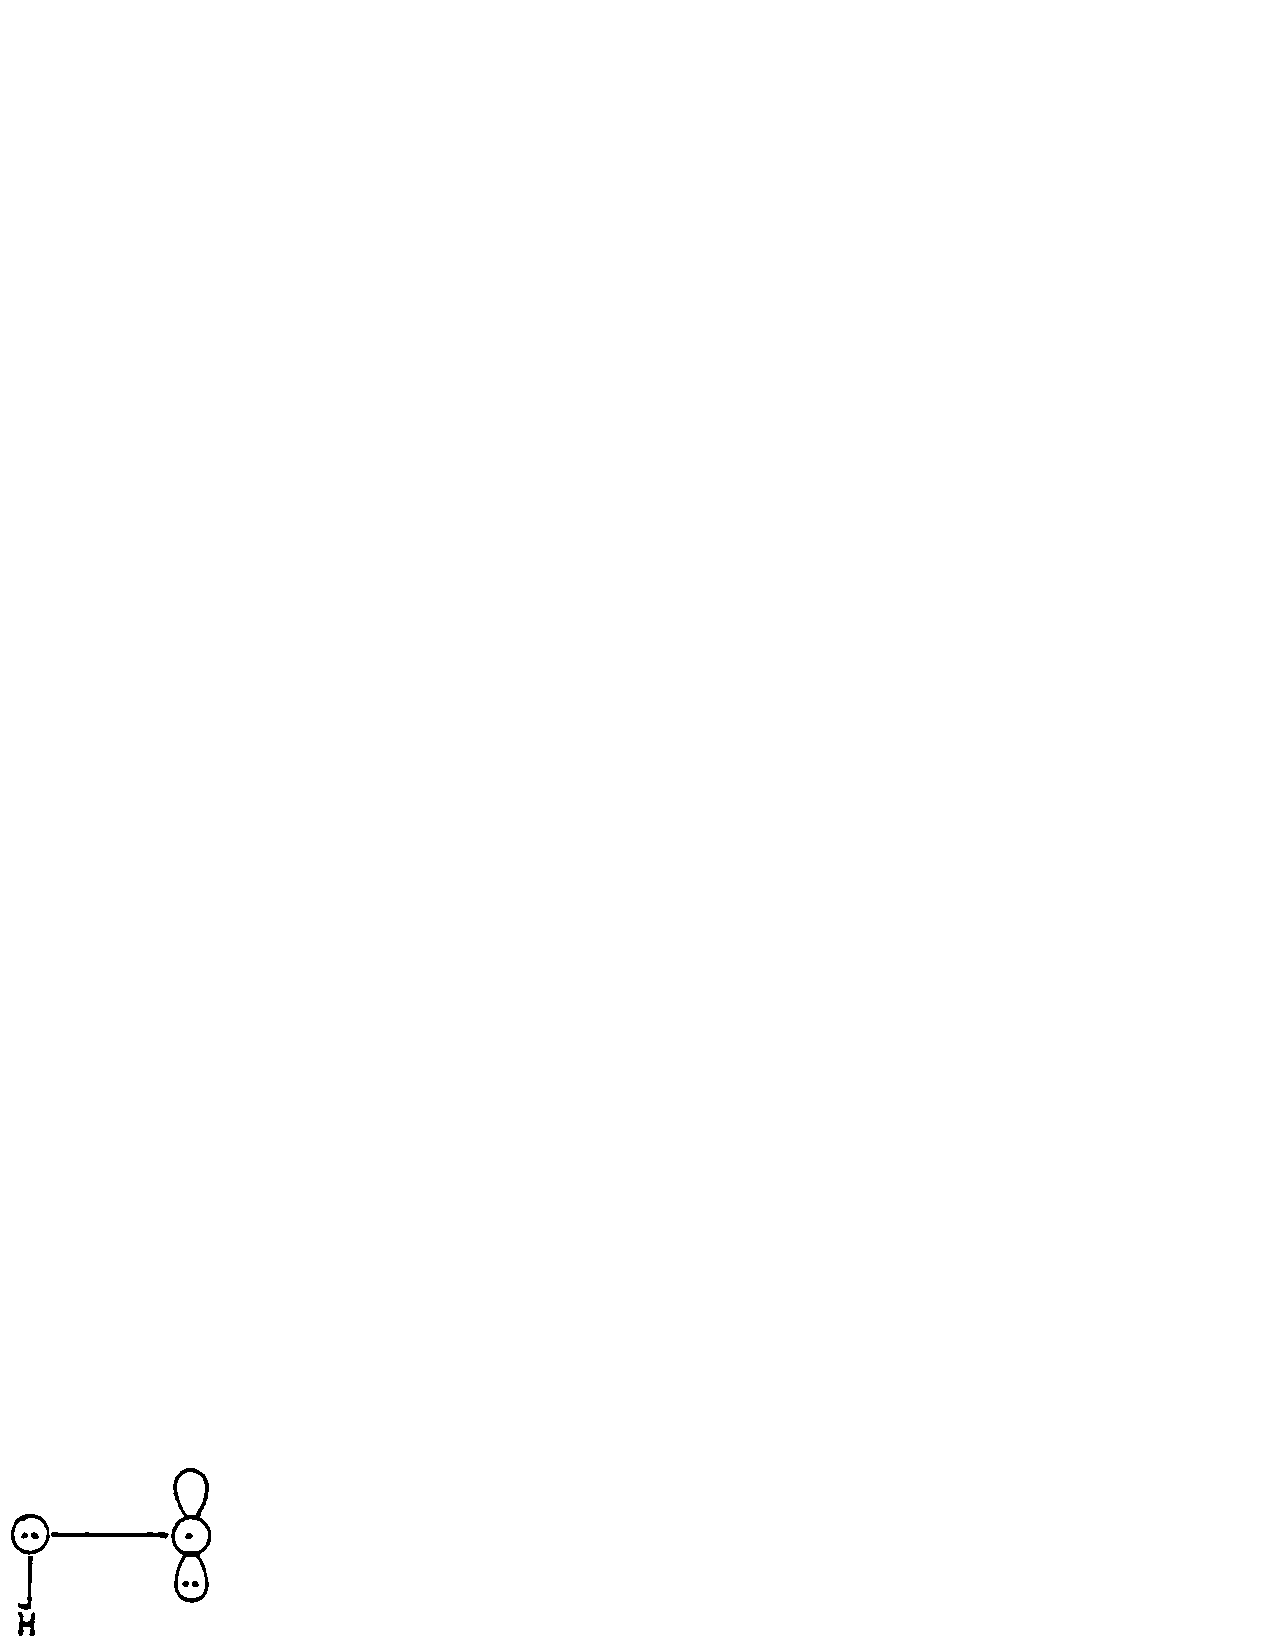
\includegraphics{fg12-19}
\label{chap12-eqno8}
\end{equation}
where the orbitals in the sigma bonds have been suppressed.  The
result is that the resonance energy in O$_2$, a good part of the 70
kcal bonding in the pi system, is lost.  Although (\ref{chap12-eqno7})
seems to have the radical electron localized on the right oxygen, the
wavefunction contains a significant amount of
\begin{equation}
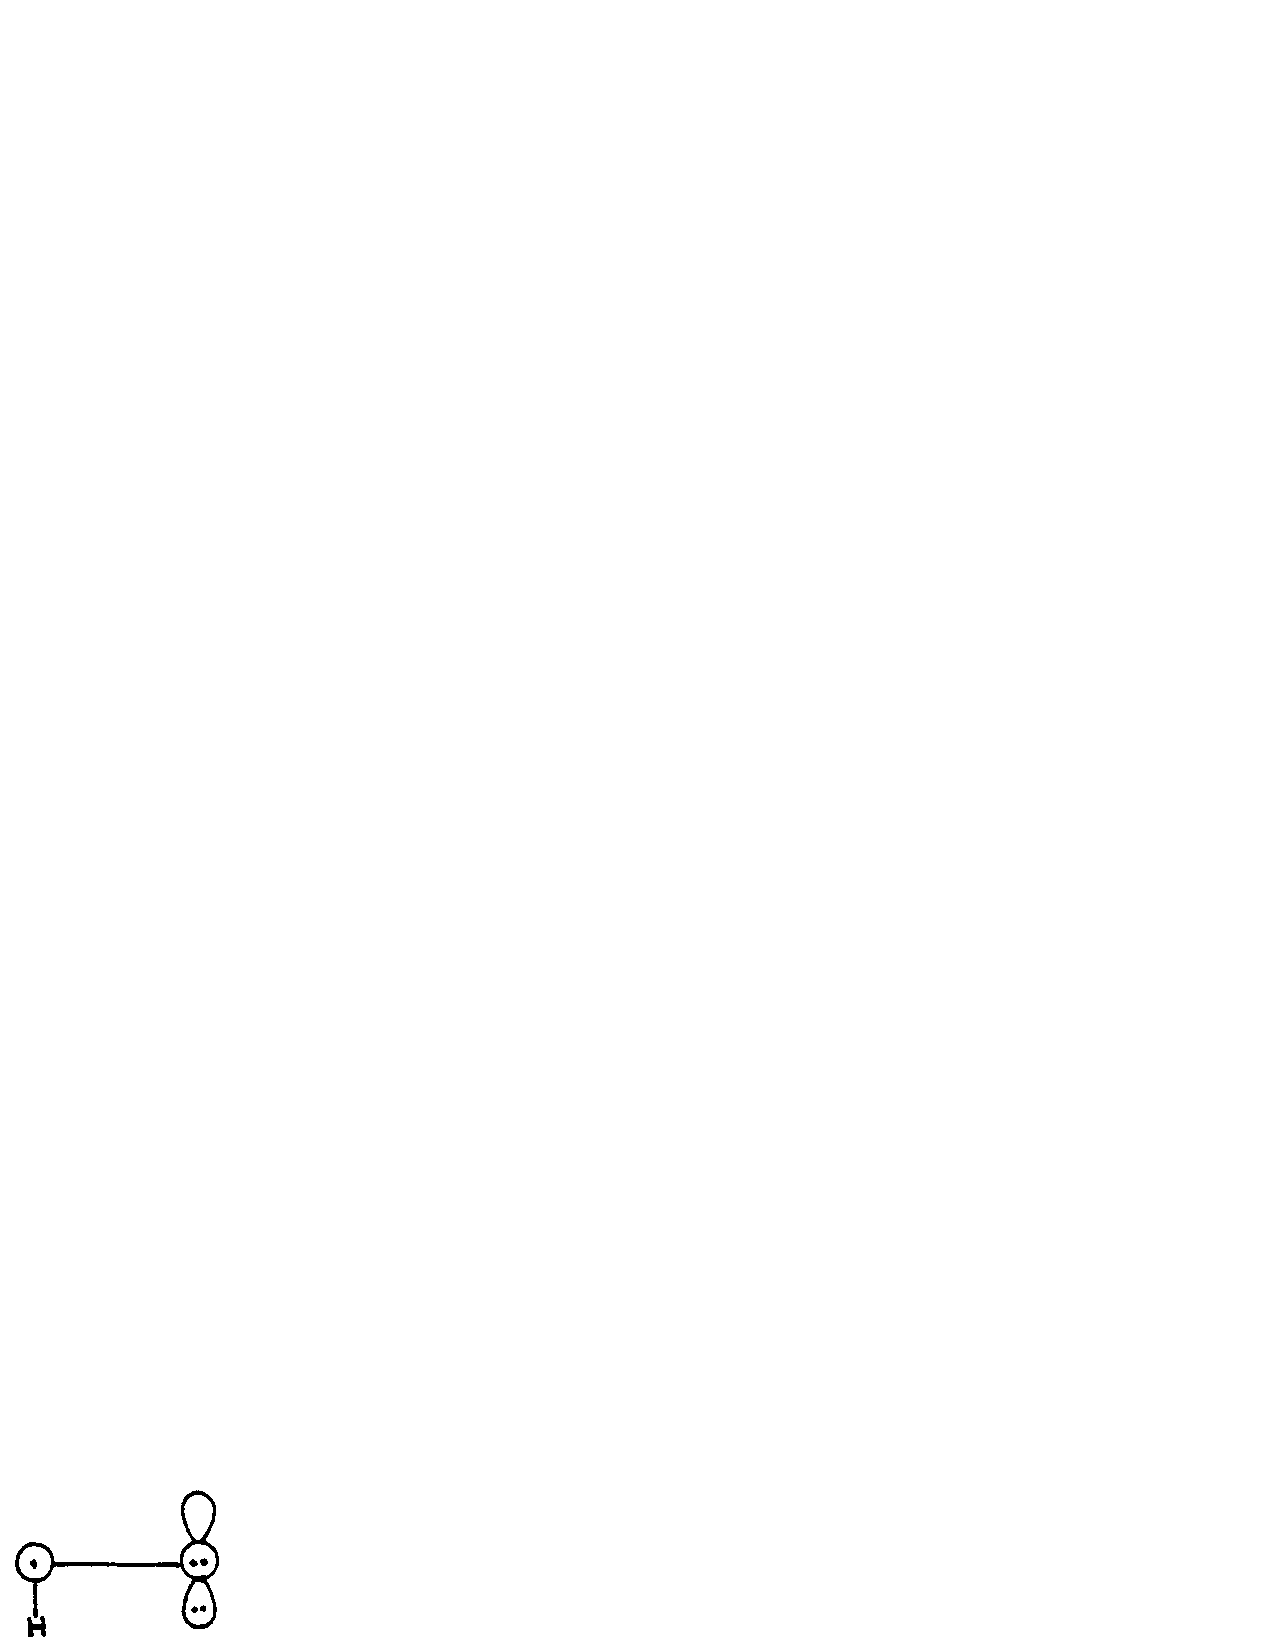
\includegraphics{fg12-20}
\label{chap12-eqno9}
\end{equation}
character.  This configuration is a mixture of the zwttterion
\begin{equation}
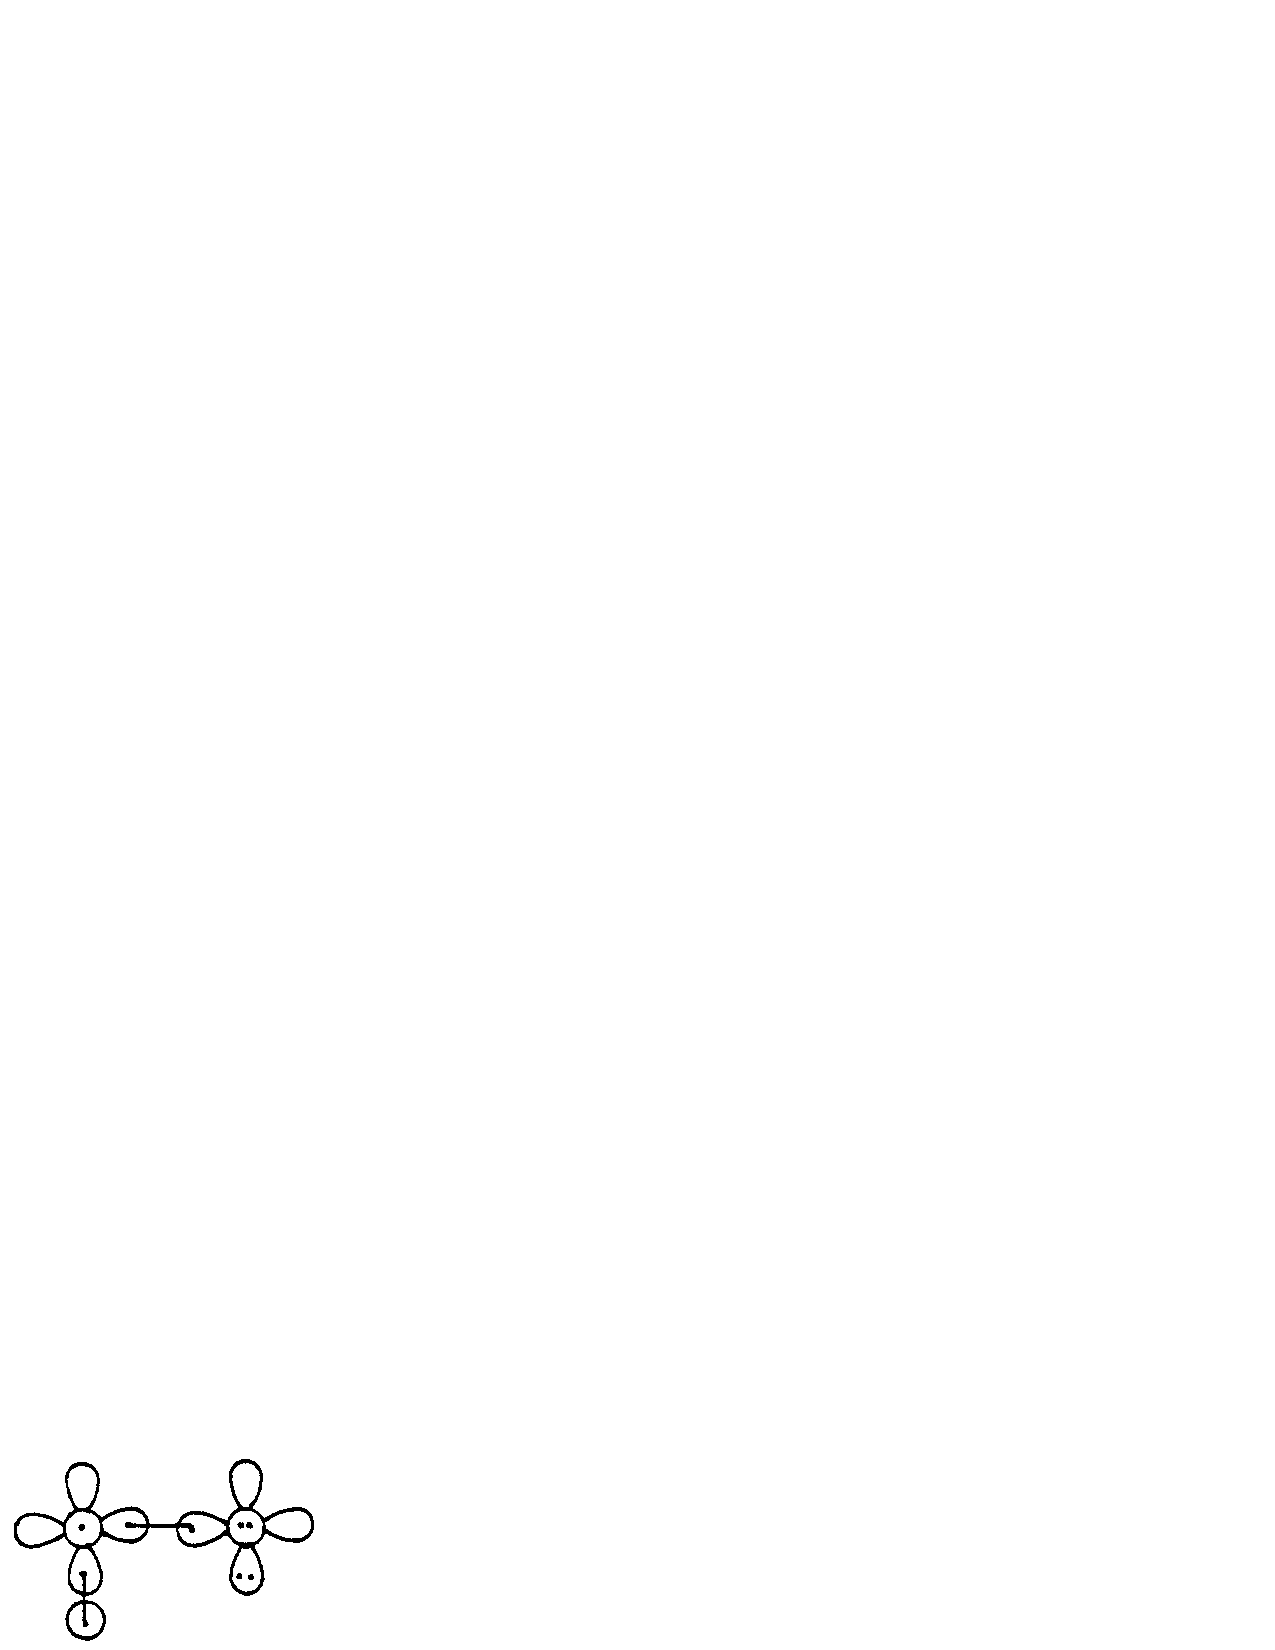
\includegraphics{fg12-21}
\label{chap12-eqno10}
\end{equation}
and the neutral configuration
\begin{equation}
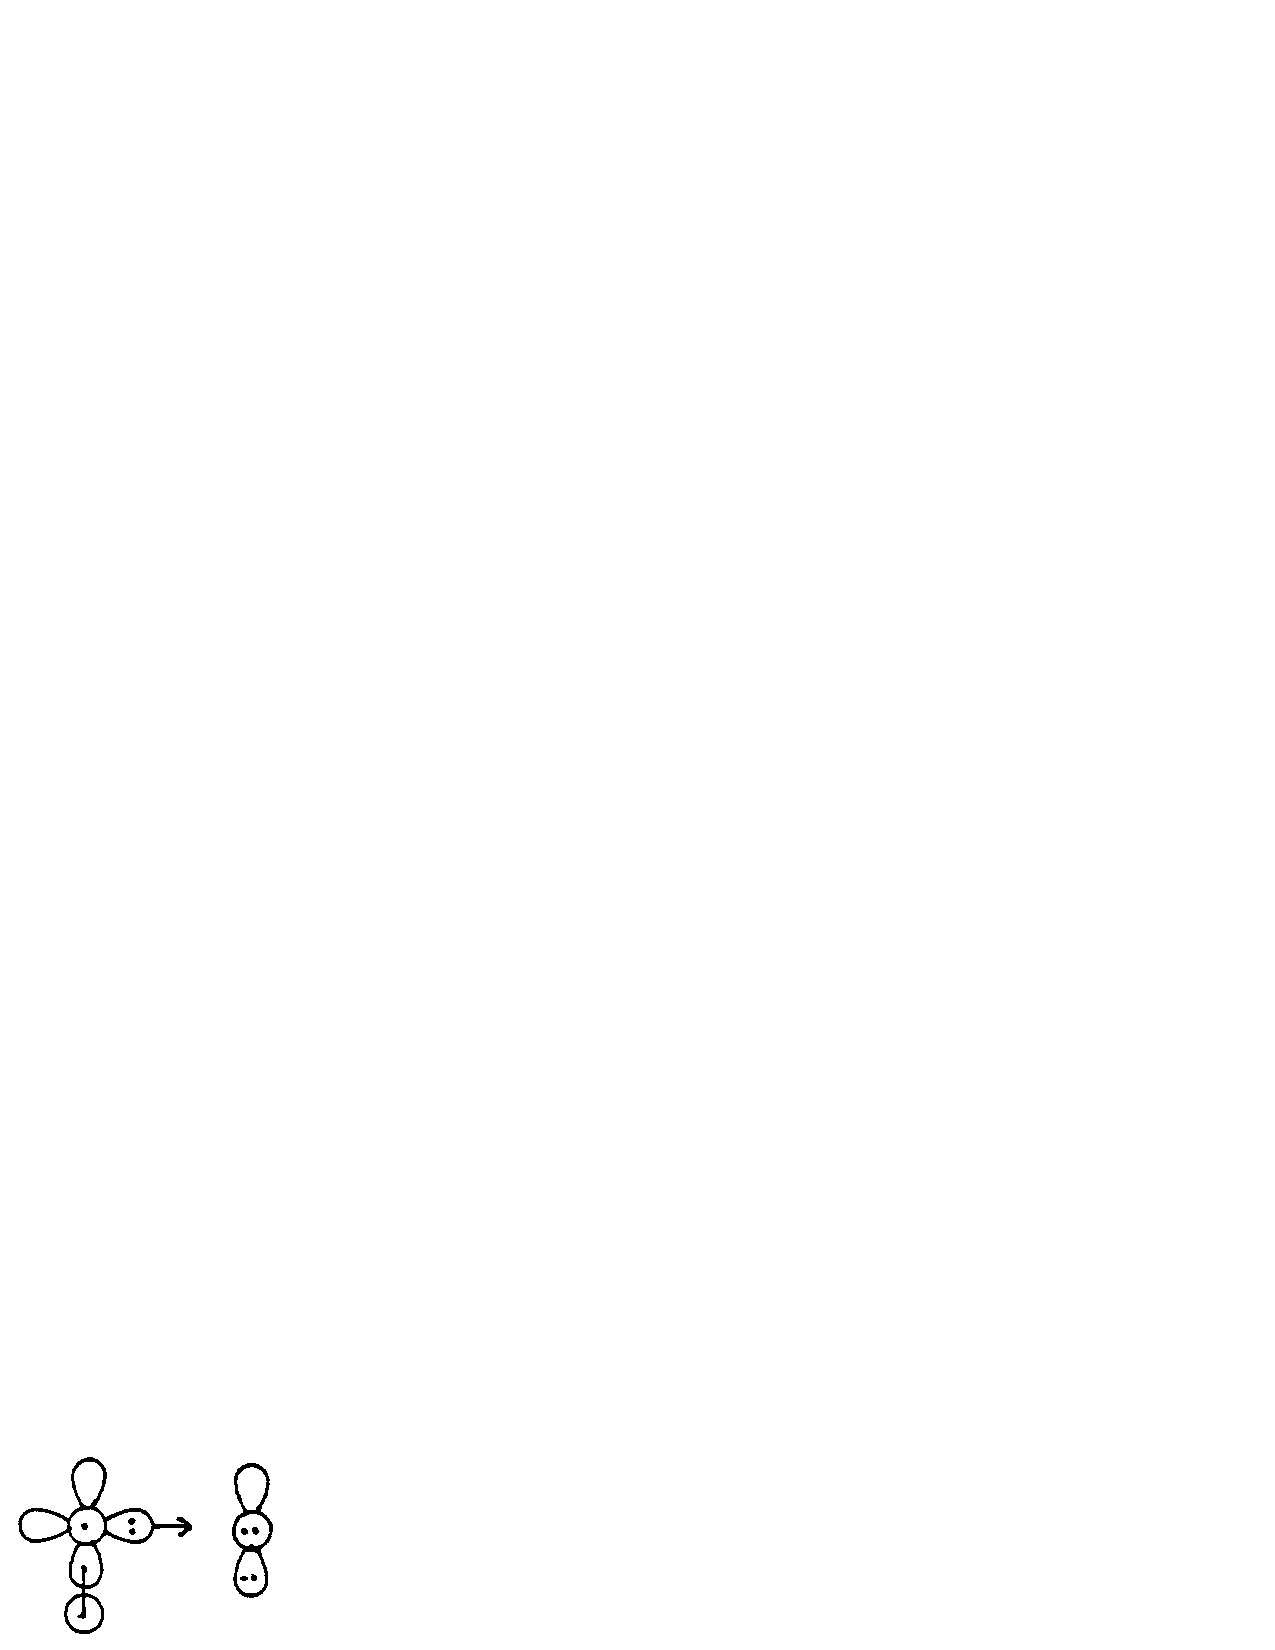
\includegraphics{fg12-22}
\label{chap12-eqno11}
\end{equation}
The result is that there is $\sim$13 kcal of pi bonding in HO$_2$.  Thus, 
the O-O bond is weakened by $\sim$57 kcal, 70$-$13, leading to an O-O 
bond for HO$_2$ of $\sim$61 kcal, 48 + 13.  Similarly, because of this 
loss of 57 kcal, the bond of H to O$_2$ is 57 kcal weaker than a normal 
H-O bond.  Since a normal H-O bond is 104 kcal, we see that the bond of 
H to O$_2$ is only 47 kcal, 104$-$57.

These results can be used to estimate the energetics for other peroxy
radicals.  Thus, considering a monovalent species R, e.g., R=CH$_3$,
NH$_2$, OH, F, SiH$_3$, PH$_2$, SH, Cl, etc., we would estimate the
bond energy of RO$_2$ as D(R$-$O$_2$) = D(R$-$OMe) $-$ 57 kcal.  A
slightly worse approximation is obtained by using D(R$-$OH) in place
of D(R$-$OMe).  Some results are indicated in Table \ref{chap12-tab9}.

\begin{table}
\caption{Bond energies D$^a_{298}$ in kcal, from 
reference 1.}
\label{chap12-tab9}
\begin{tabular}{cccc}\\ \hline
R & D(R-OMe) & D(R-OH) & D(R-O$_2$)\cr

H & 103.6 & 119.2 & 47.0\cr
CH$_3$ & 80.7 & 90.5 & (24.0)\cr
NH$_2$ &\cr
OH & (44.0) & 51.2 & ($-$3.0)\cr
F &\cr
SiH$_3$ &\cr
PH$_2$ &\cr
SH &\cr
Cl &\cr
\hline
\end{tabular}
\end{table}

\subsubsection{Ozone}

Consider now bonding an O atom to O$_2$ to form ozone. Starting with one 
configuration of ground state O$_2$
\begin{equation}
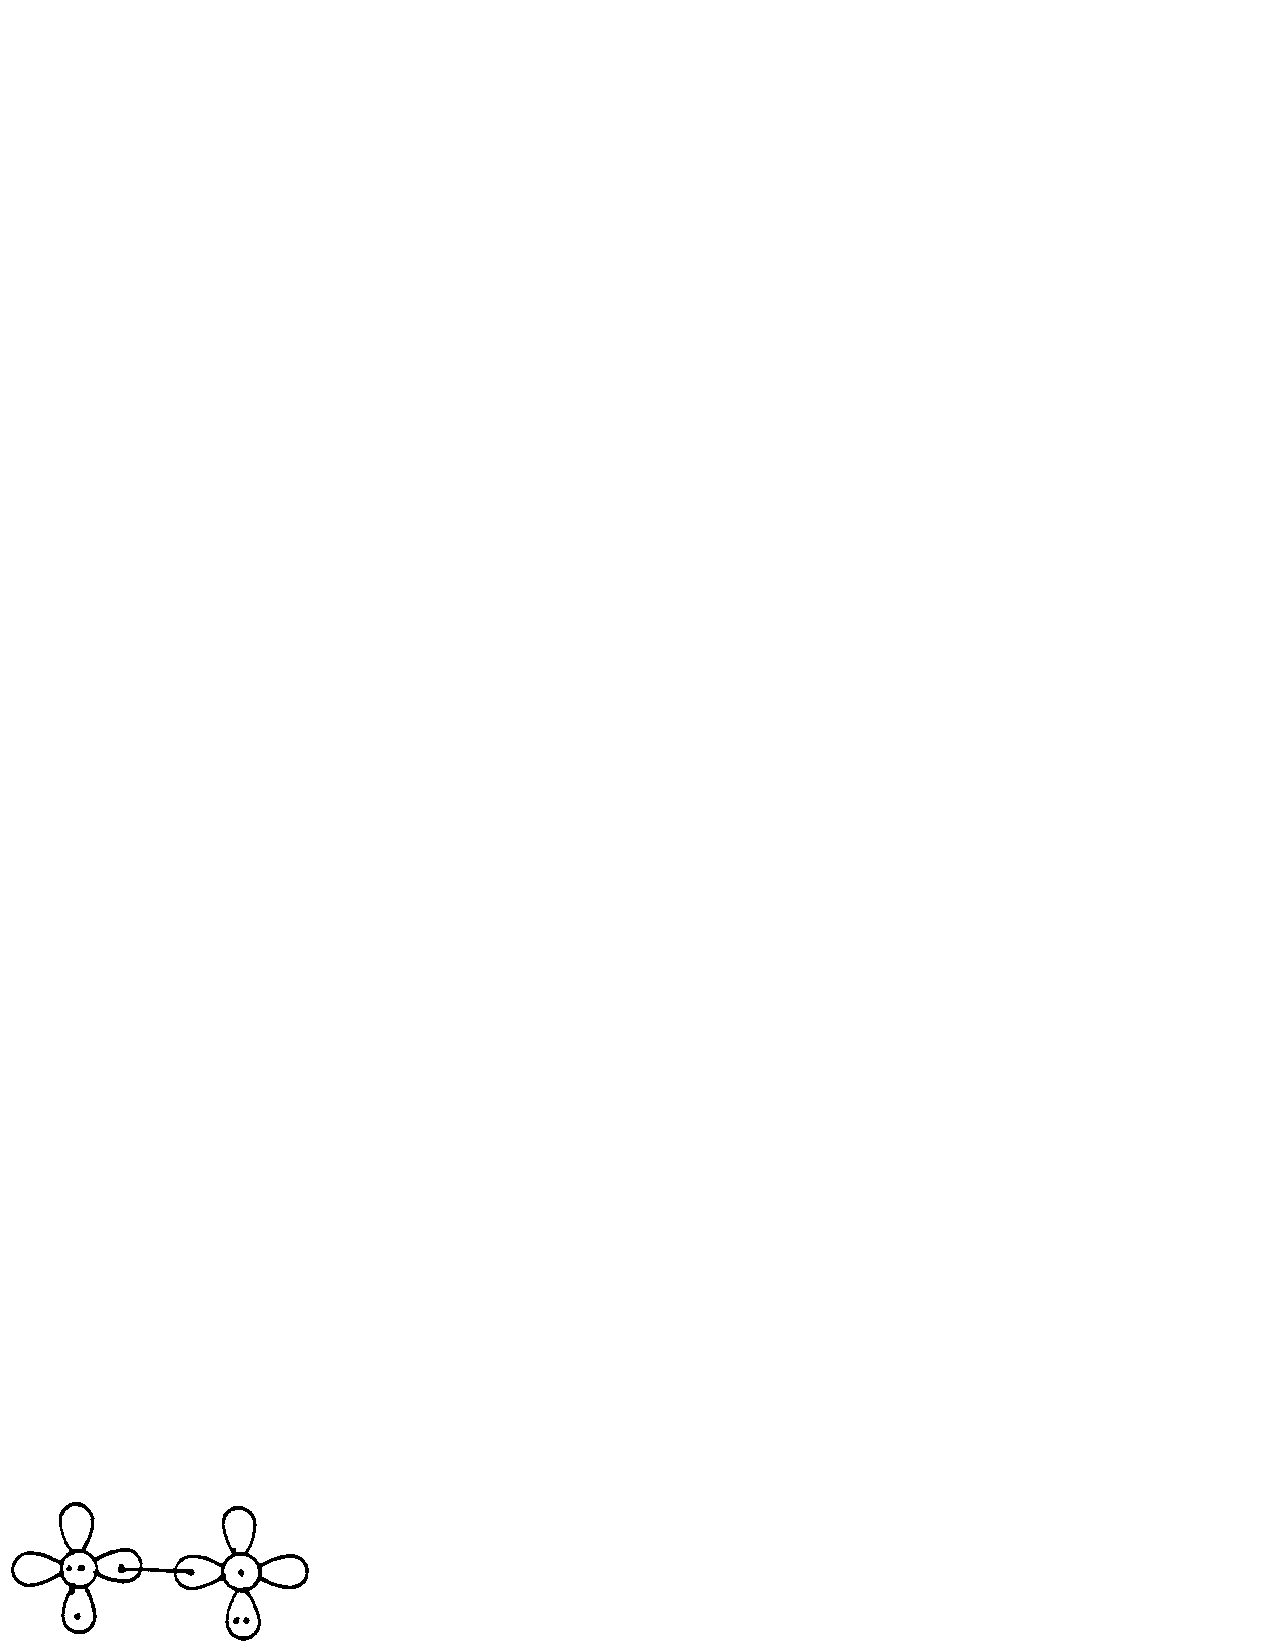
\includegraphics{fg12-23}
\label{chap12-eqno12}
\end{equation}
and binding an O atom leads to two favorable configurations, the
4$\pi$
\begin{equation}
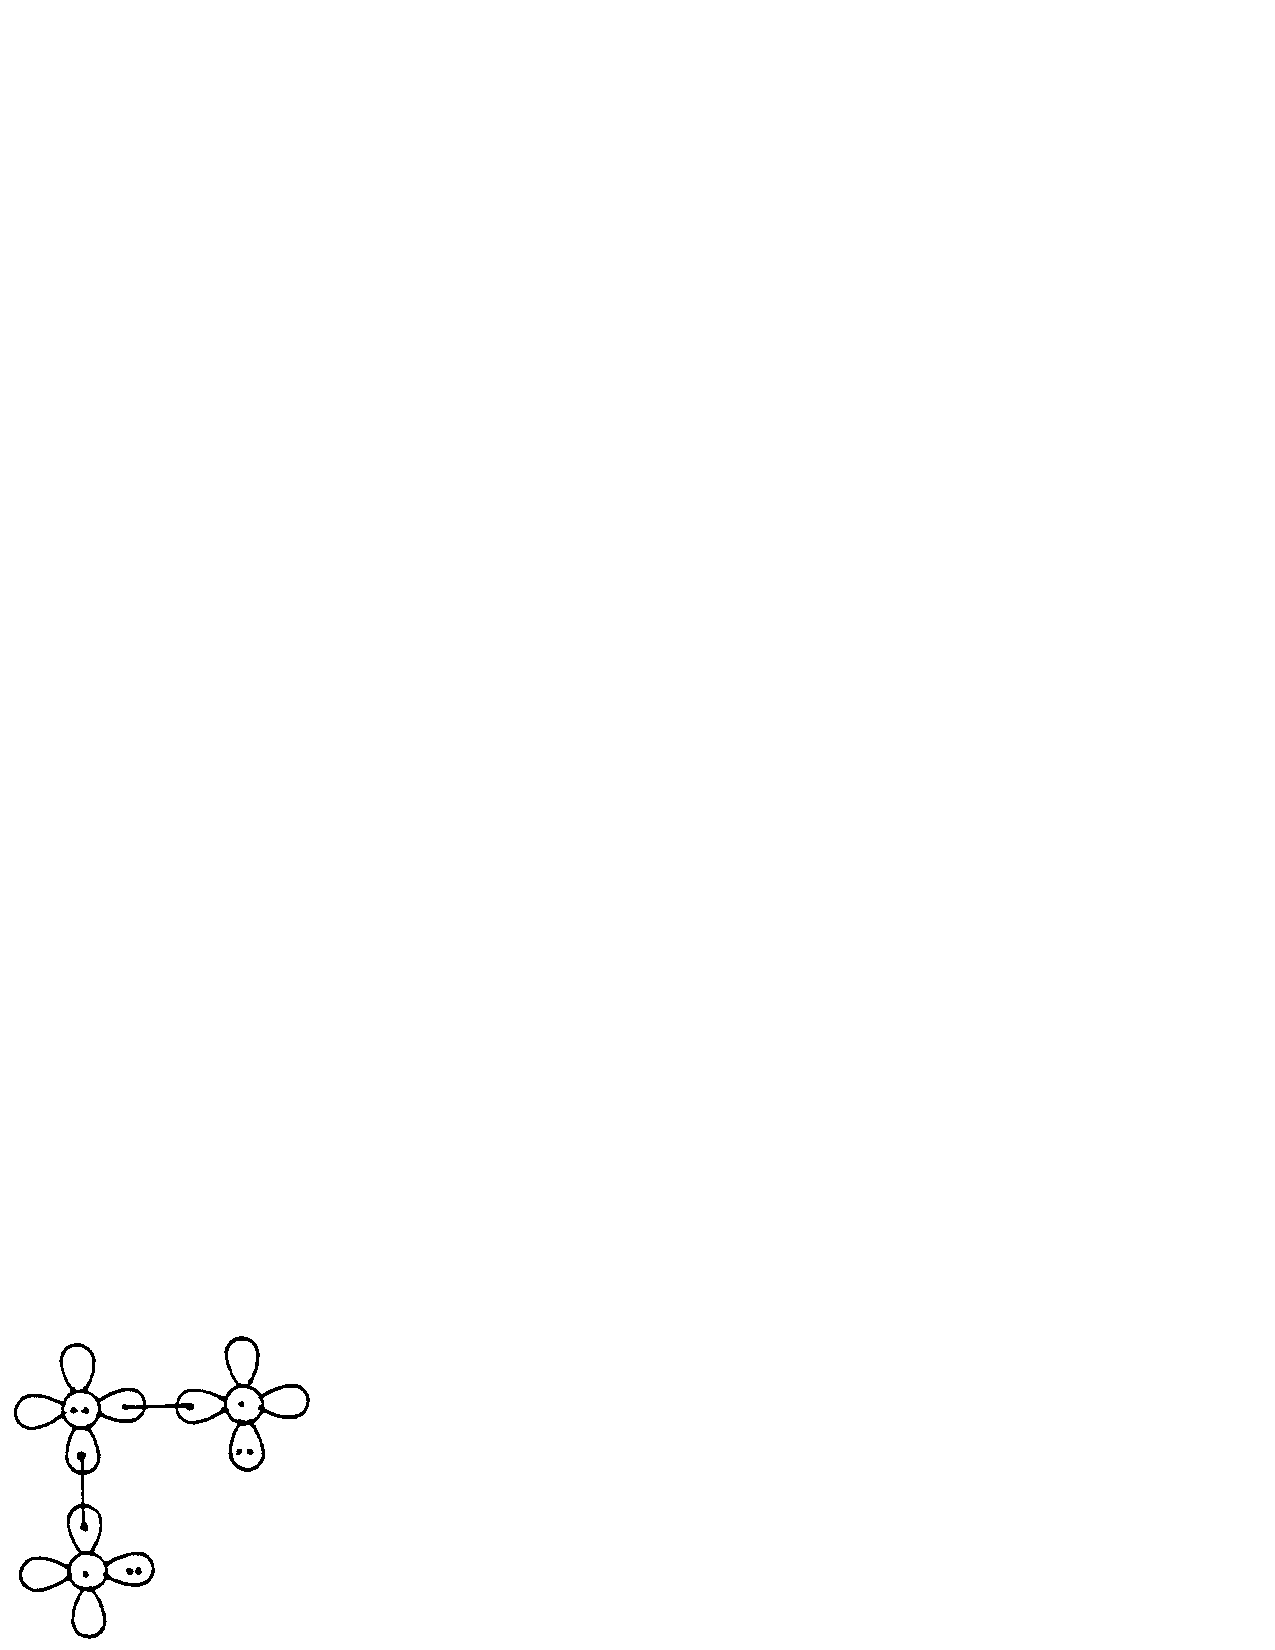
\includegraphics{fg12-24}
\label{chap12-eqno13}
\end{equation}
and the 5$\pi$
\begin{equation}
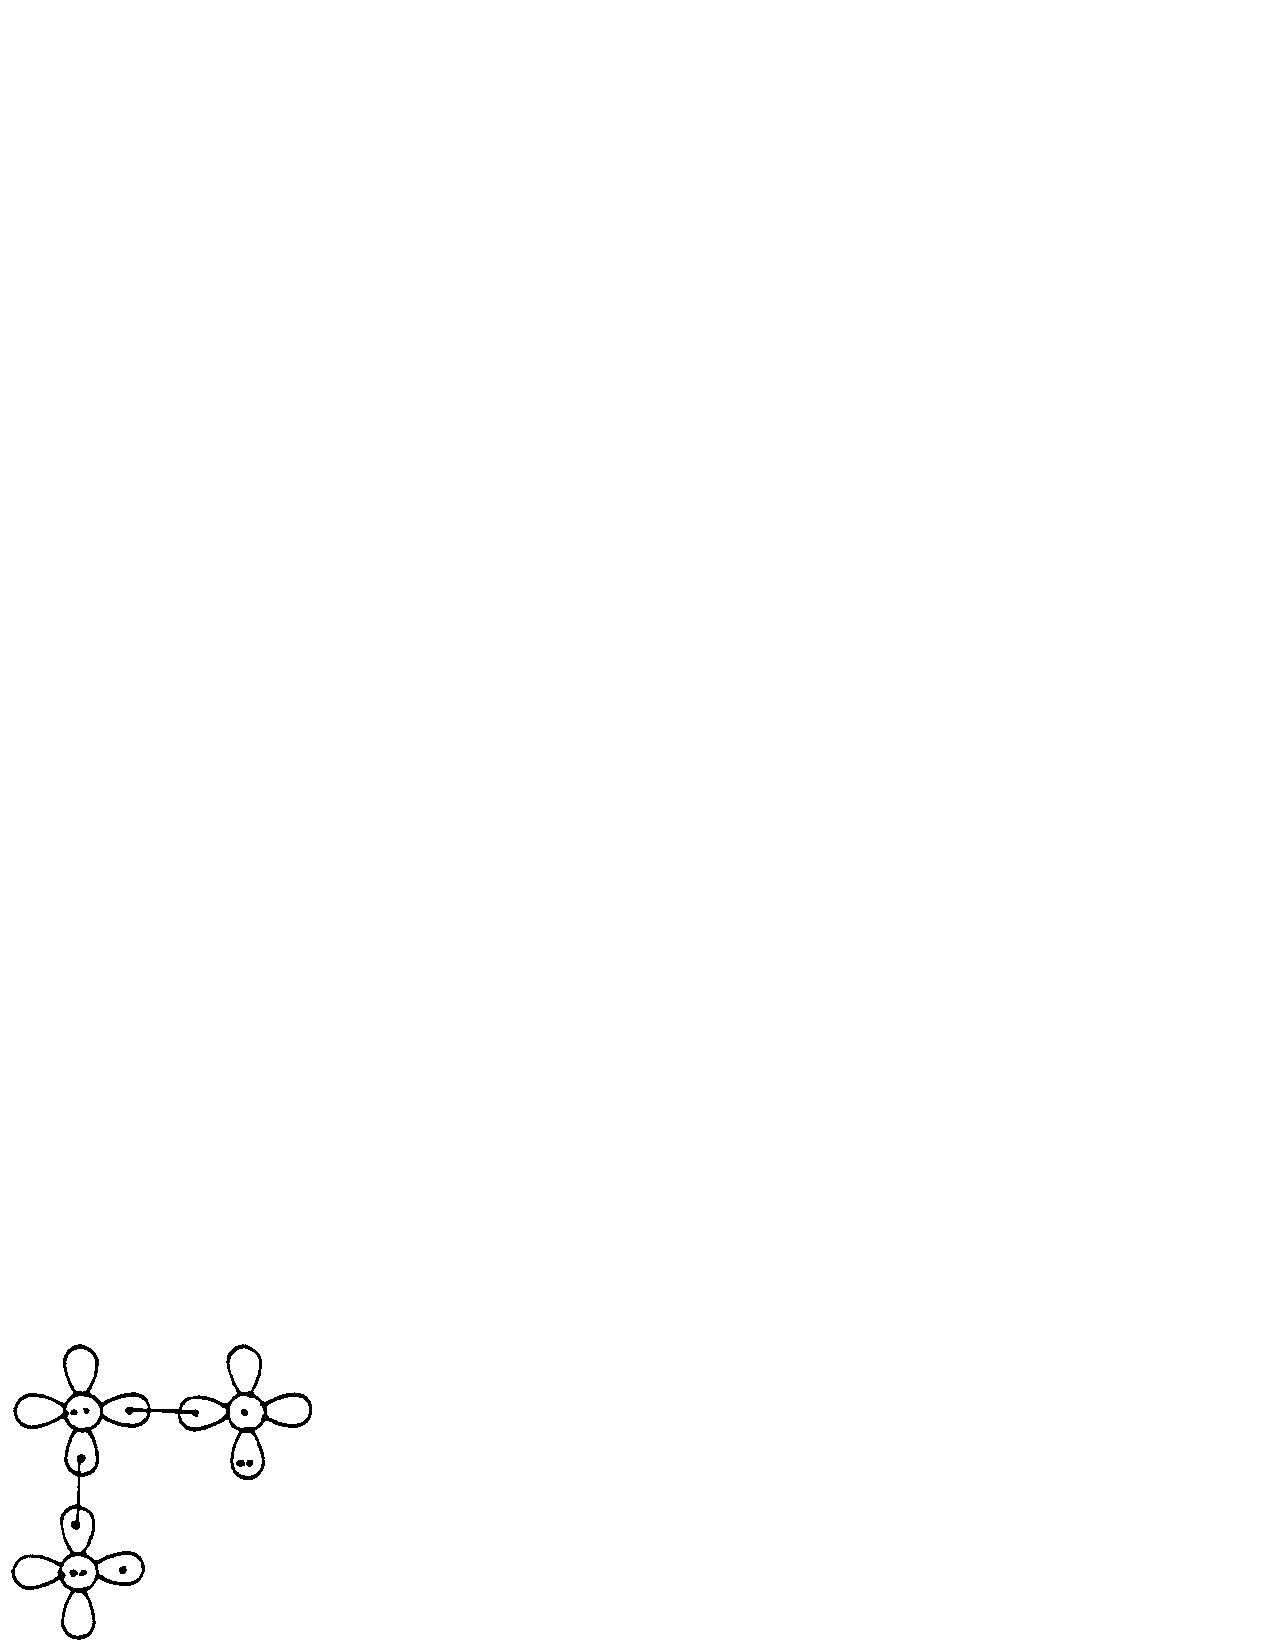
\includegraphics{fg12-25}
\label{chap12-eqno14}
\end{equation}
These configurations are denoted $4 \pi$ and $5\pi$, respectively, 
indicating how many elections are in $\pi$ orbitals.

Based on previous considerations, we expect the new O-O sigma bond to
be worth 48 kcal, but decreased by the loss of 57 kcal of pi bonding
in the O$_2$. Thus, ozone would be unbound by 9 kcal.  This analysis
is approximately correct for configuration (\ref{chap12-eqno14}), but
not for (\ref{chap12-eqno13}).

Since the new atom in (\ref{chap12-eqno13}) has a singly occupied
$\pi$ orbital, we also obtain a new three-electron pi bond worth
$\sim$13 kcal. This would lead to a net bond of $\sim$4 kcal. There is
another major effect however.  Configuration (\ref{chap12-eqno13}) has
two singly occupied $\pi$ orbitals, one on each terminal atom.
Denoting these orbitals as $\phi_{\ell}$ and $\phi_{r}$, we can
construct both a singlet state
\begin{equation}
\left( \phi_{\ell} \phi_r + \phi_r \phi_{\ell} \right) \left( \alpha 
\beta - \beta \alpha \right)
\label{chap12-eqno15}
\end{equation}
and a triplet state
\begin{equation}
\left( \phi_{\ell} \phi_r + \phi_r \phi_{\ell} \right) = 
\cases{( \alpha \alpha )&\cr
(\alpha \beta + \beta \alpha )&\cr
(\beta \beta)&\cr}
\label{chap12-eqno16}
\end{equation}
If the $\phi_{\ell}$ and $\phi_r$ orbitals were orthogonal, the
triplet state would be lower.  However, for (\ref{chap12-eqno13})
there is an overlap between $\phi_{\ell}$ and $\phi_r$, stabilizing
the singlet state.

Since the terminal atoms are far apart, we would not expect a large 
overlap, 0.04 for atomic
orbitals, and hence, not much of a bond. However, the doubly occupied 
p$\pi$ orbital on the central atom
couples the $\ell$ and $r$ orbitals leading to a large overlap and a large bonding 
effect. The three-electron pi
bond in HO$_2$ arises from mixing of the configuration
\begin{equation}
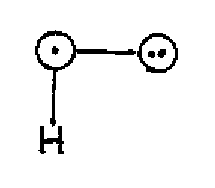
\includegraphics{fg12-26-1}
\label{chap12-eqno17}
\end{equation}
into the dominant configuration
\begin{equation}
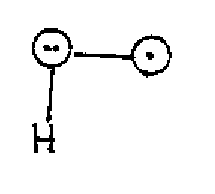
\includegraphics{fg12-26-2}
\label{chap12-eqno18}
\end{equation}
For O$_3$ the three-electron pi bonds to the $r$ atom lead to a second 
zwitterion configuration of the form
\begin{equation}
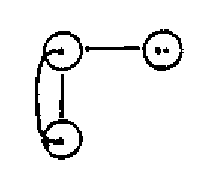
\includegraphics{fg12-27-1}
\label{chap12-eqno19}
\end{equation}
and hence, a strong pi bond to the $\ell$ atom.  Similarly the three-electron 
pi bond to the $\ell$ atom leads to the configuration
\begin{equation}
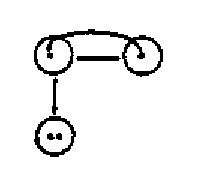
\includegraphics{fg12-27-2}
\label{chap12-eqno20}
\end{equation}
and hence, a strong pi bond to the $r$ atom.  Configurations
(\ref{chap12-eqno19}) and (\ref{chap12-eqno20}) appear to incorporate
ionic character.  However, there are also readjustments in the sigma
system, there are also readjustments in the sigma system, leading to
more covalent charge distribution.  The result of mixing
(\ref{chap12-eqno19}) and (\ref{chap12-eqno20}) with the dominant
configuration (\ref{chap12-eqno13}) or
\begin{equation}
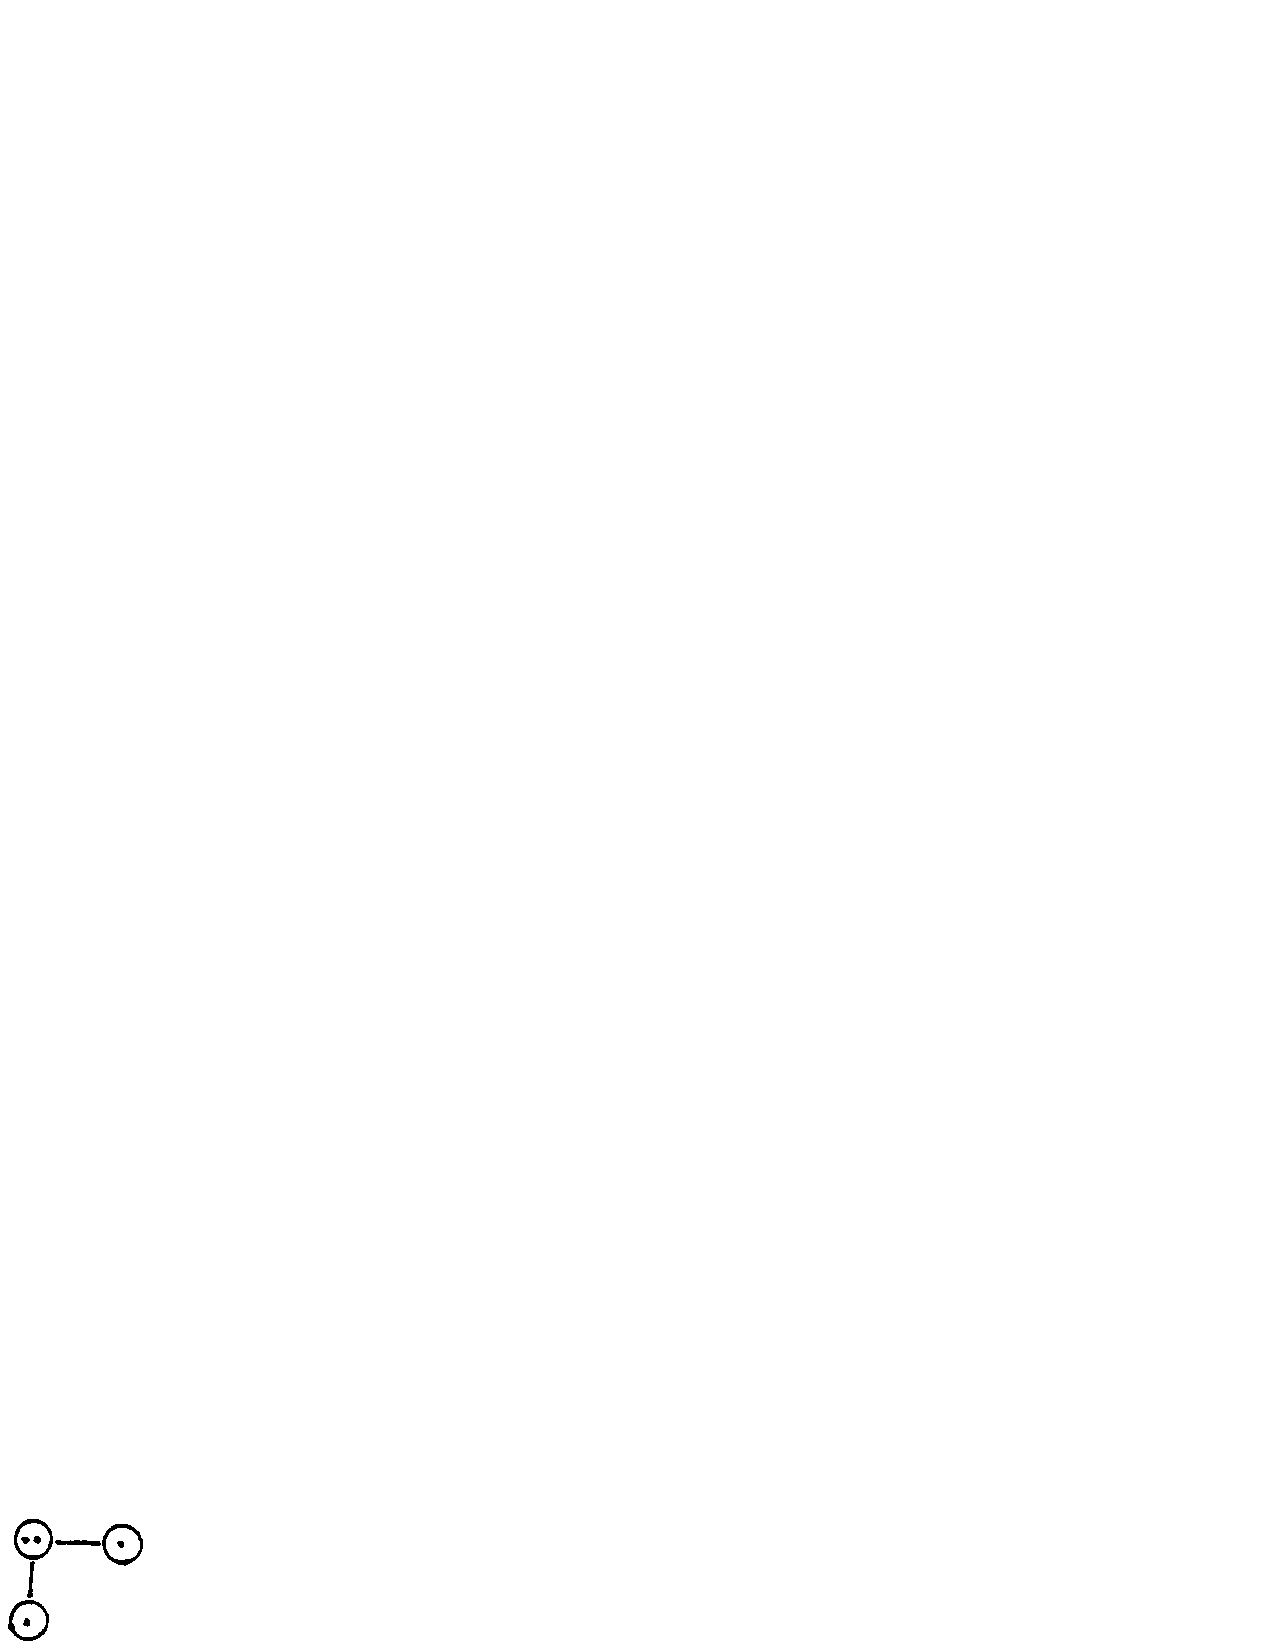
\includegraphics{fg12-28}
\label{chap12-eqno22}
\end{equation}
is a strong stabilization of the singlet state, which leads to a net bond of 
24.2 kcal.

In the generalized valence bond description, the superposition of
configurations (\ref{chap12-eqno19}) + (\ref{chap12-eqno20}) +
(\ref{chap12-eqno22}) is replaced by one configuration in which the
orbitals are allowed to delocalize.  The resulting orbitals are shown
in Figure \ref{chap12-fig1}.  Here we see that: the O2s orbitals
ignored in this description do not change quantitatively; each
terminal atom has a $p$ lone pair in the molecular plane; the O-O
sigma bonds are composed of paired $p$ orbitals; and, the p$\pi$
orbitals are a slightly delocalized form of (\ref{chap12-eqno22}).

The above analysis suggests that the OOO bond angle should be
90$^{\circ}$.  Indeed, examination of Figure \ref{chap12-fig1}(c)
shows that the orbitals in the central O atom are at
90$^{\circ}$. However, considering the $p$ lone pairs in Figure
\ref{chap12-fig1}(b), we see that the orbitals lead to repulsive
interaction between the terminal atoms causing the bond to open
up. The final bond angle is 116.8$^{\circ}$.


\begin{figure}
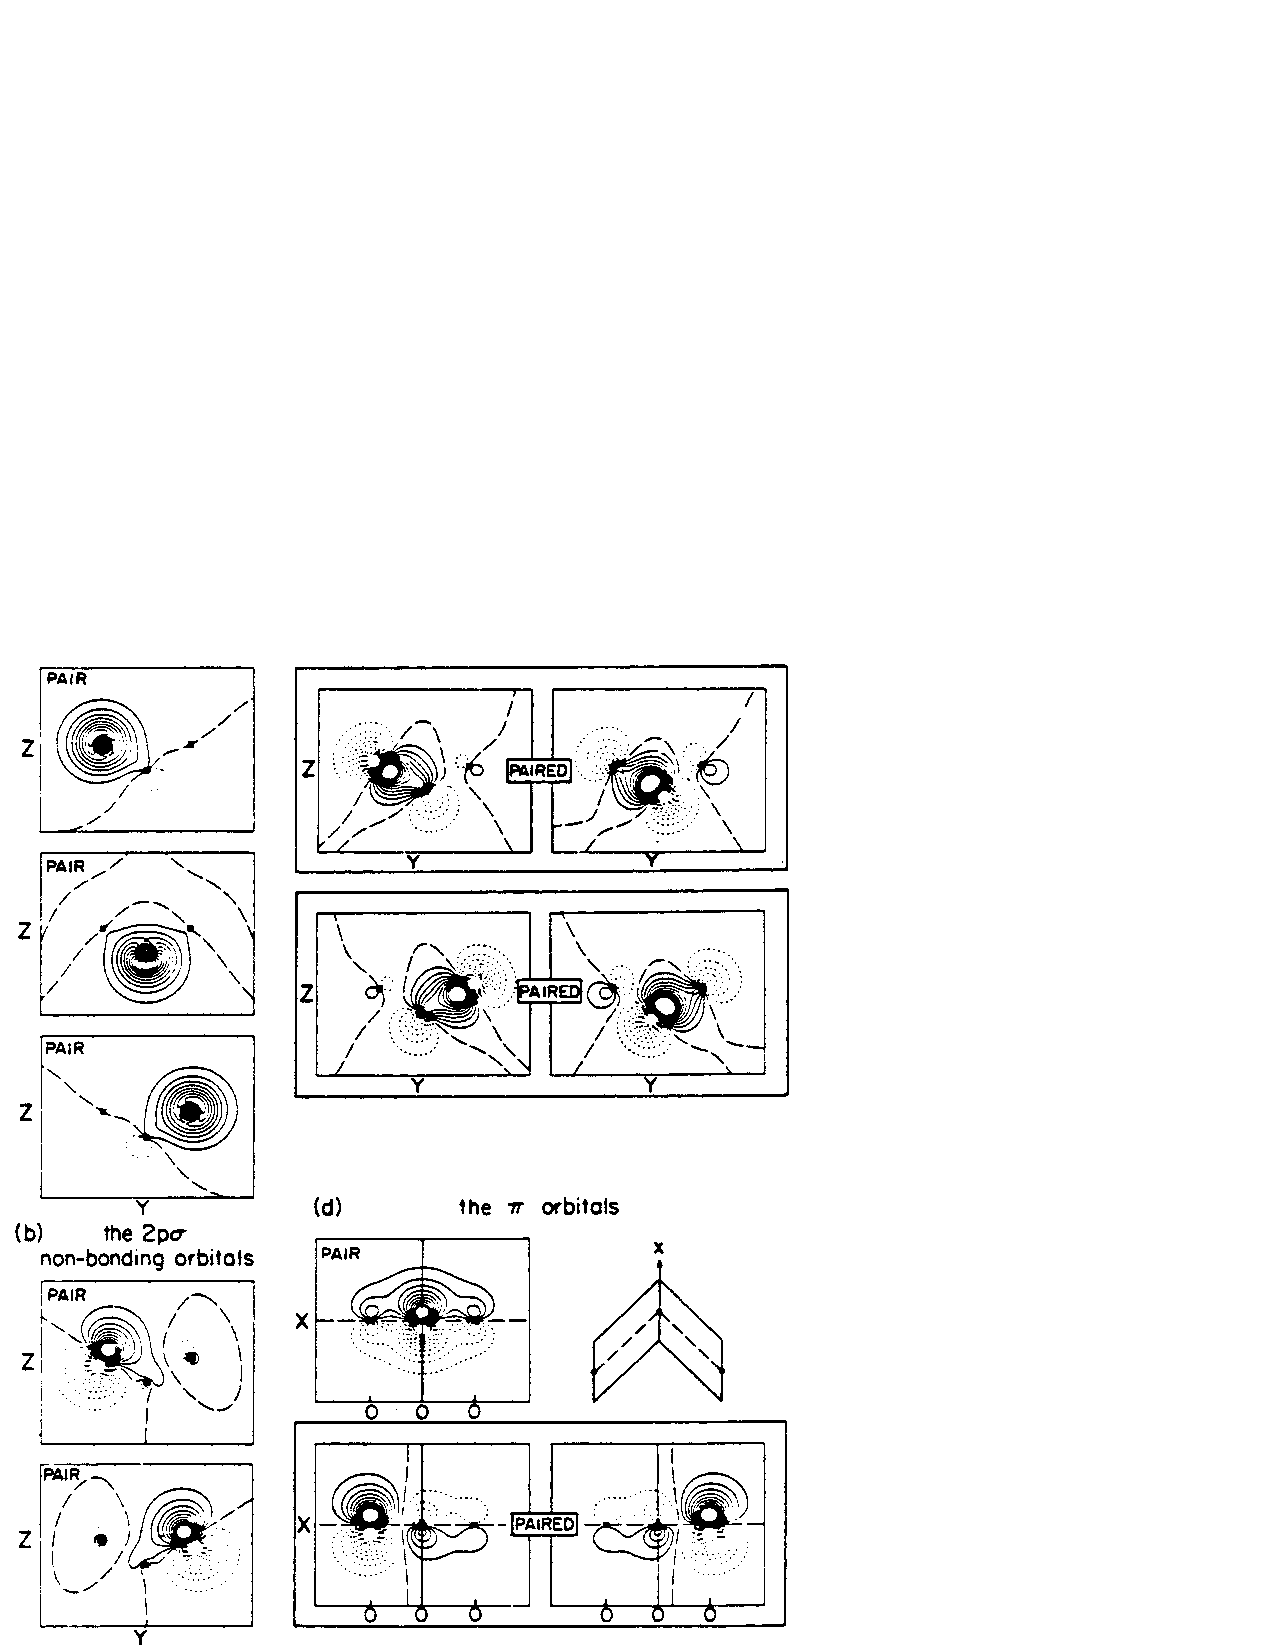
\includegraphics[scale=0.75]{fg12-30}
\caption{The calculated GVB orbitals of 
ozone (${^1A}_1$ state).  The contour increment is 0.05 atomic units.}
\label{chap12-fig1}
\end{figure}

\begin{table}
\caption{OO bond lengths.}
\label{chap12-tab10}
\begin{tabular}{cc}\\ \hline
O$_2$ & 1.208\AA\cr
O$_3$ & 1.272\AA\cr
HO$_2$ & 1.335\AA\cr
HOOH & 1.465\AA\cr
\hline
\end{tabular}
\end{table}

The bond length of ozone is compared in Table \ref{chap12-tab10} with
those of related systems.  As is consistent with the extra $\pi$
bonding in O$_3$, the O-O bond length is 0.06
\AA\ shorter than in HO$_2$, but 0.06 \AA\ larger than in O$_2$.

The cohesive energy of ground-state ozone is 24.2 + 118.0 = 142.2 kcal. 
Since the average O-O
sigma bond is 48 kcal, the $\pi$ system of ozone contributes $\sim$46 kcal of 
bond energy.  Since a three-electron pi bond is worth 13 kcal, from 
HO$_2$, we can consider this 46 kcal of pi bonding to be two
three-electron pi bonds, 26 kcal total, plus 20 kcal from singlet pairing 
of the $\ell$ and $r$ orbitals.  Indeed,
at the ground state geometry the triplet state is 1.6 eV = 37 kcal above 
the singlet suggesting about
18 or 19 kcal of bonding between the $\ell$ and $r$ orbitals, since 
in the case of small overlap the singlet-triplet
separation of a biradical pair is twice the bond energy in the singlet.

\subsubsection{Metallic Forms, Te, Po, and $\alpha$Se}

Crystalline Te has a trigonal crystal structure, A8 type. This is
referred to as metallic Te but actually it has an energy gap of 0.36
eV and hence, should be referred to as a semiconductor.  The structure
posses infinite spirals of Te atoms, two bonds to each atom, with
weaker bonds between spirals.  Each atom has an additional four bonds
involving three other spirals, see Figure \ref{chap12-fig2}.  The
spiral repeats every three atoms.  The stable form, $\alpha$, of Se, a
dark grey, semi-metallic crystal, has the same crystal structure and
an energy gap of 2.3 eV.

\begin{figure}
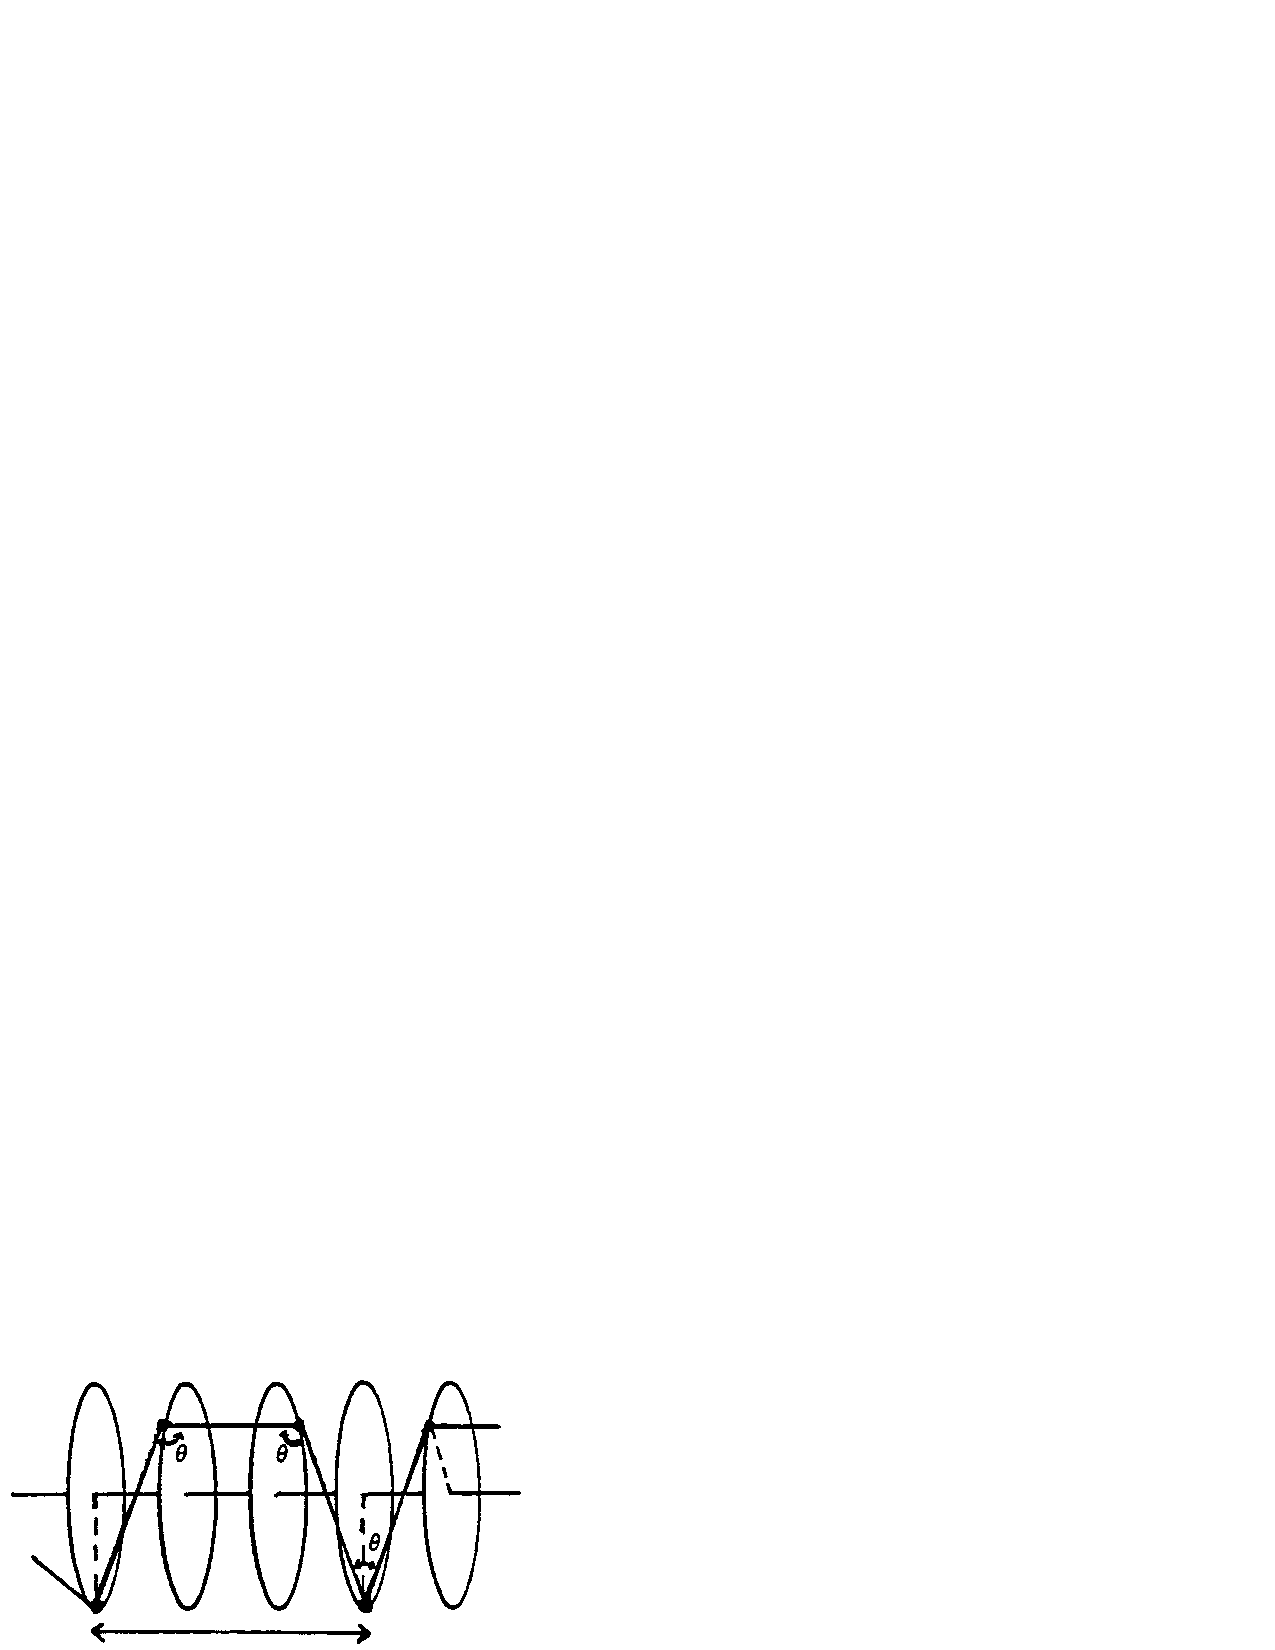
\includegraphics[scale=0.75]{fg12-31}
\caption{The crystal structure of Te and $\alpha$-Se.}
\label{chap12-fig2}
\end{figure}

There are two crystalline forms of Po, both metallic with six covalent
bonds to each atom.  $\alpha$-Po is simple cubic with one atom per 
cell, a = 3.366 and $\theta = 90^{\circ}$, and $\beta$-Po is rhombohedral 
with one atom per cell, a = 3.373 and $\theta = 98.1^{\circ}$.

Upon heating, $\alpha \rightarrow \beta$ at 54$^{\circ}$C, while upon 
cooling, $\beta \rightarrow \alpha$ at 18$^{\circ}$C.
\begin{equation}
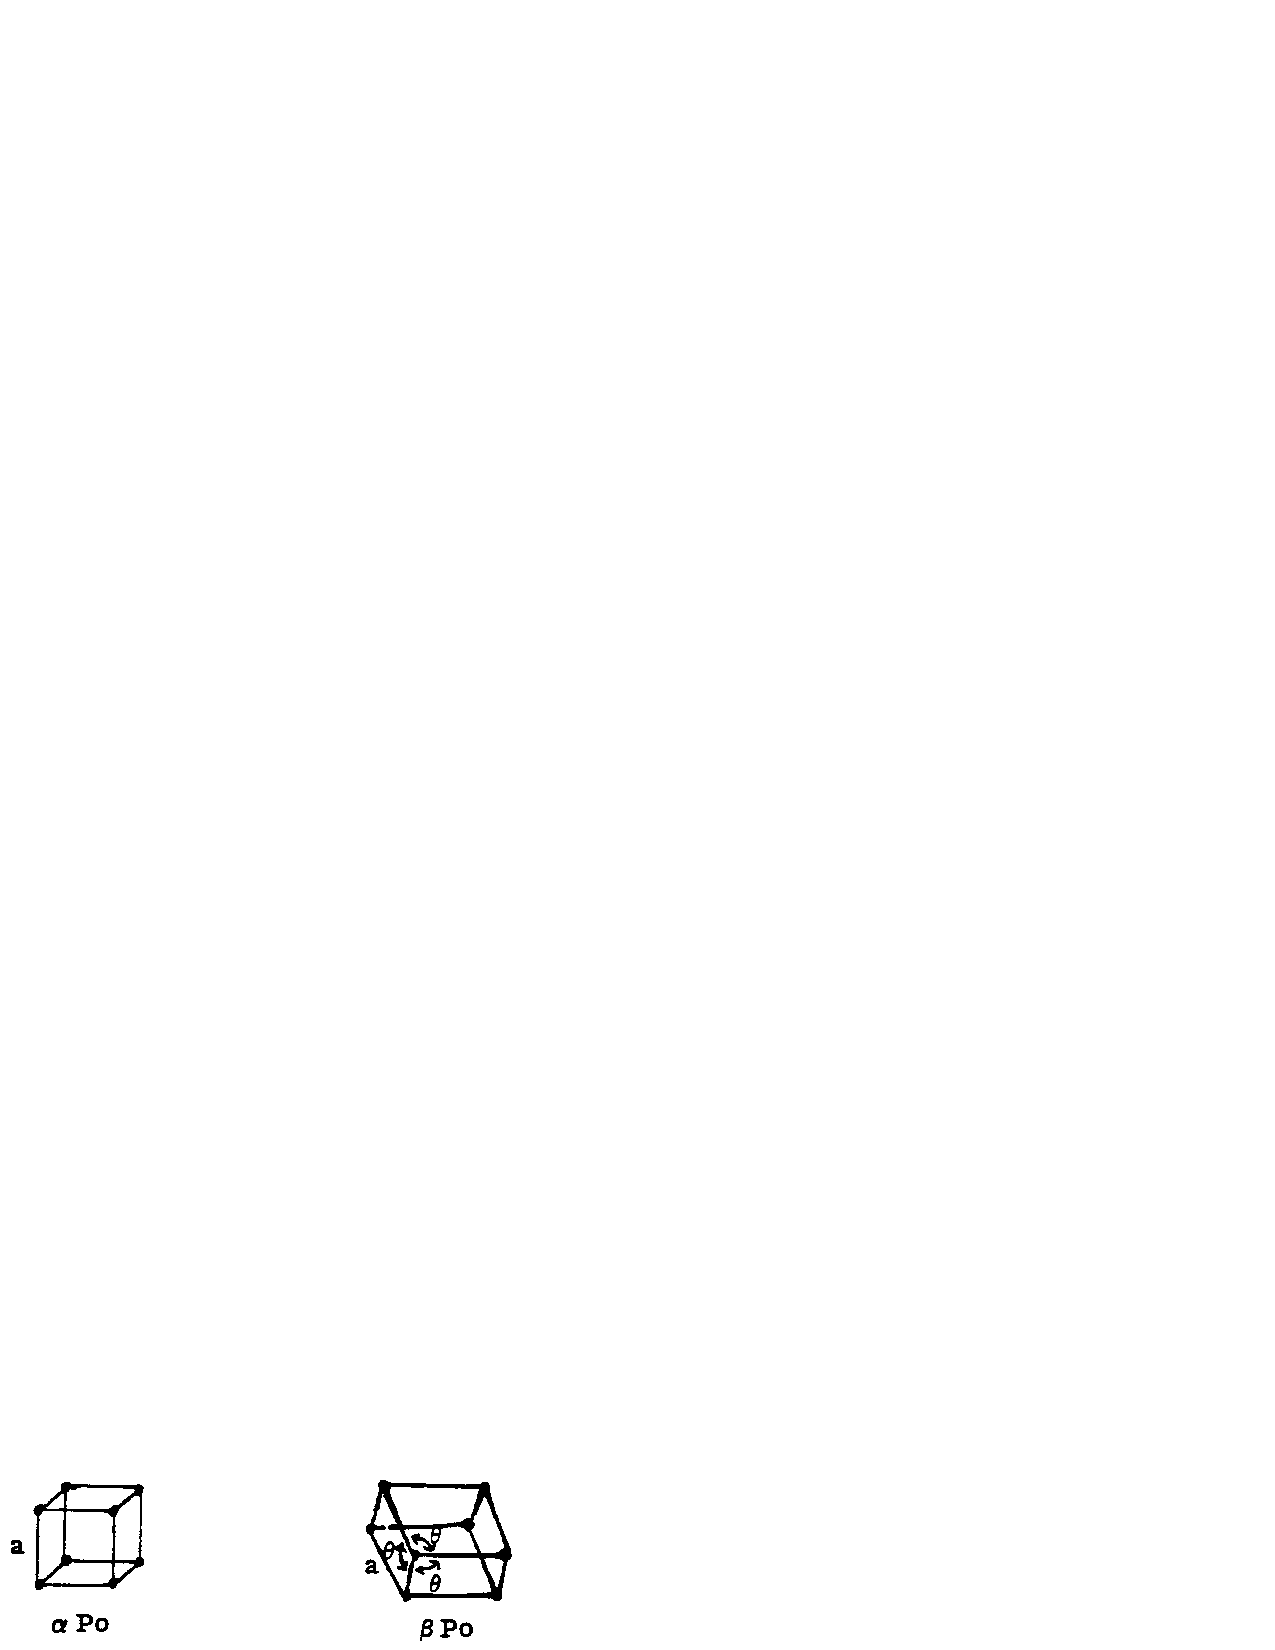
\includegraphics{fg12-32}
\end{equation}
The cubic form, $\alpha$-Po, can be considered as a special case of the Te 
structure with $\theta = 90^{\circ}$, and six equal bonds rather than two 
short and four long.  Little is known about the properties of Po metal
since all isotopes have radioactive nuclei. The most readily available 
isotope is $^{210}$Po which decays by $\alpha$ emission with a half-life 
of 138.4 days. Indeed, the radioactivity leads to an equilibrium 
temperature of 500$^{\circ}$C for a capsule containing a half gram 
of $^{210}$Po.

Parameters for these structures are compared in Table
\ref{chap12-tab11}. We will consider the bond length within the
spirals as the length of a single bond. In all three cases the bonds
between, spirals are comparable.  Thus, proceeding from Se, to Te, to
Po, the primary bond length gradually increases to the length of the
secondary bond.

\begin{table}
\caption{Structural parameters for metallic 
forms of Se, Te, and Po.$^a$}
\label{chap12-tab11}
\begin{tabular}{cccccc}\\ \hline
&\multicolumn{2}{c}{Within Spirals}&\multicolumn{2}{c}{Between 
Spirals}&vdW\cr
&\multicolumn{2}{c}{Two Bonds} & \multicolumn{2}{c}{Four 
bonds} & Radius\cr
& Length & Angle & Angle$^b$ & Length\cr

Se (hex)&2.374 $\pm$ 0.005&103.1 $\pm$ 0.2$^{\circ}$&100.7 $\pm$ 
0.1&3.436&4.0\cr
Te (hex)&2.834 $\pm$ 0.002&103.2 $\pm$ 0.1$^{\circ}$ & &3.494&4.4\cr
Po (cubic)&3.366&90$^{\circ}$ & & 3.366\cr
\hline
\end{tabular}\\
$^a$Reference 4.
$^b$Torsion angle.
\end{table}

\subsubsection{Other Forms of Se}

There are two other crystalline forms of Se, referred to as $\alpha$-monoclinic 
and $\beta$-monoclinic.  Both are red with a monoclinic crystal structure, 
and both involve puckered Se$_8$ rings with the crown
geometry
\begin{equation}
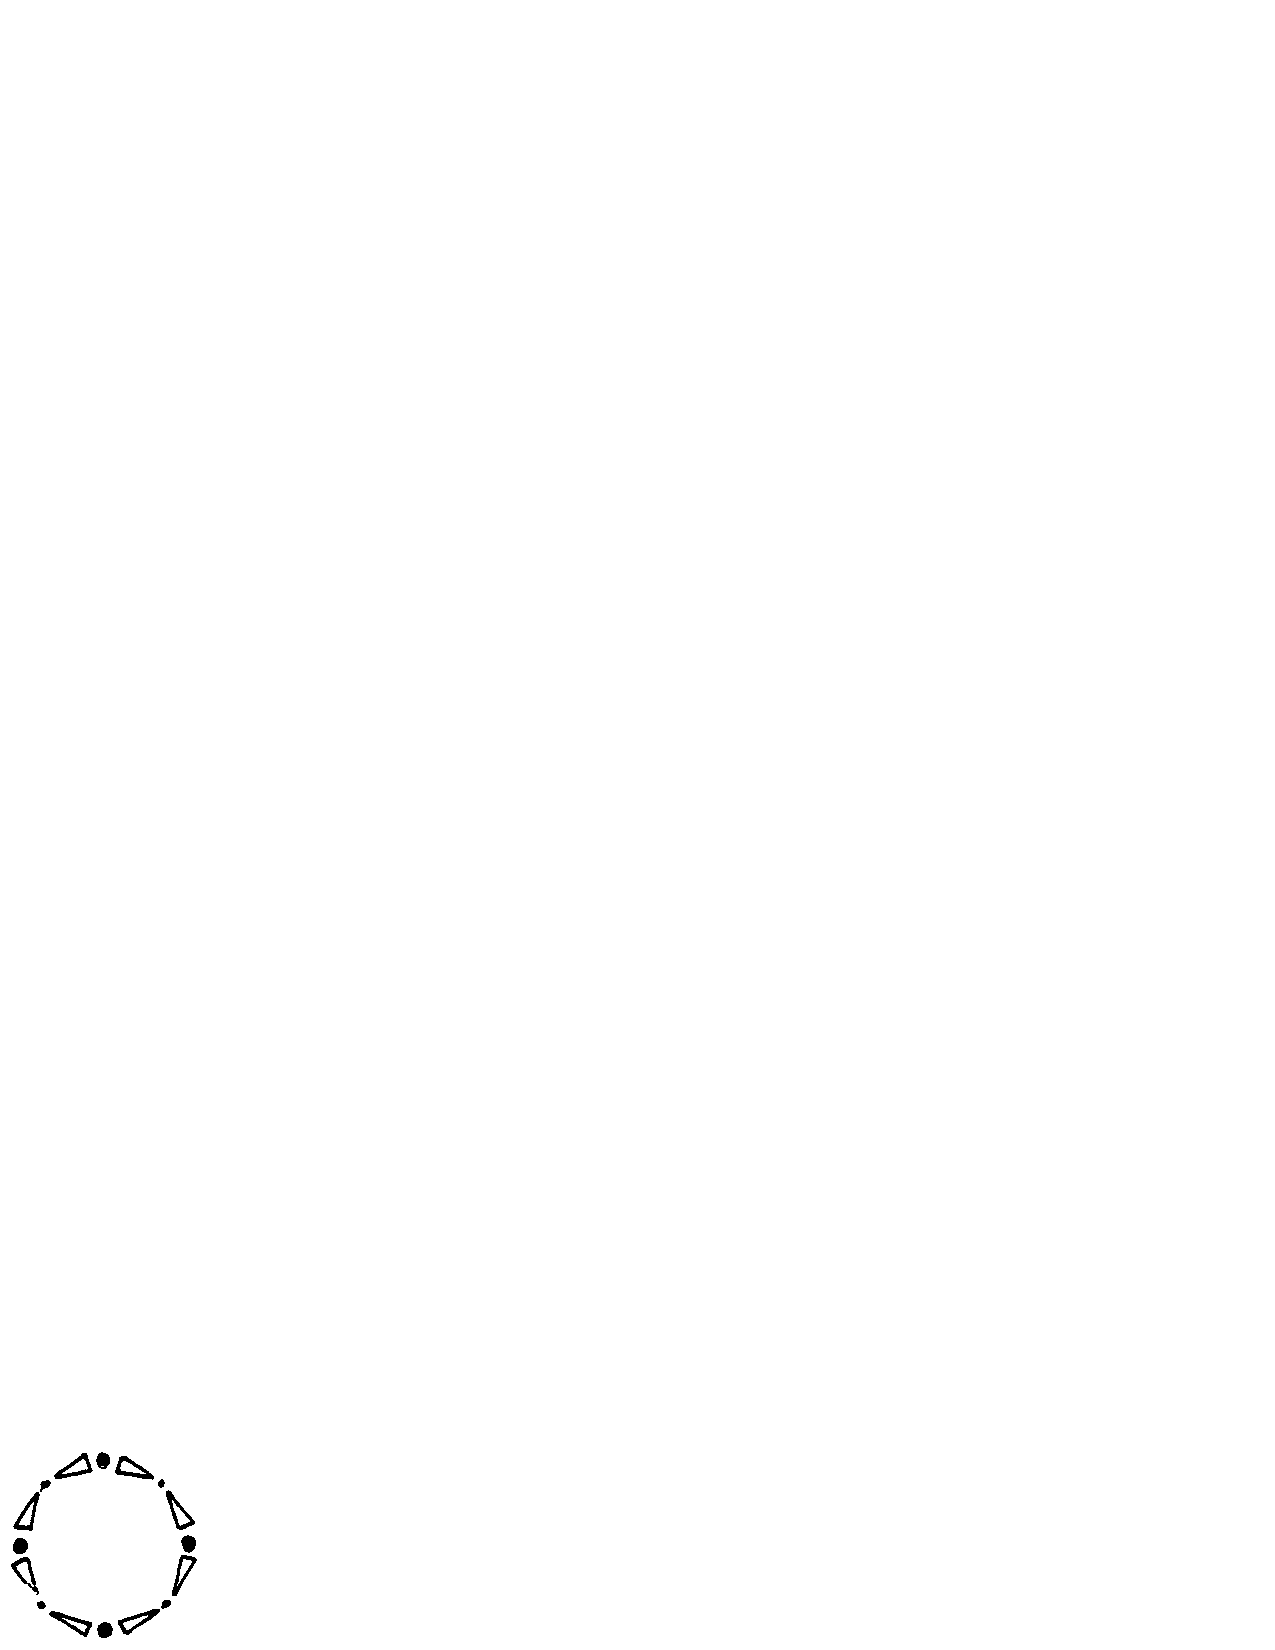
\includegraphics{fg12-33}
\label{chap12-eqno23}
\end{equation}
In both forms these rings are packed with average distances between atoms 
on different rings of 3.80 \AA.

The ordinary form of Se is amorphous, or vitreous Se, and consists of helical 
chains having Se-Se bonds of length 2.33 \AA.

\subsubsection{Other Forms of S}

Sulfur can form a number of gaseous molecules S$_n$.  Of these, S$_8$ 
is the most stable.  For $n > 4$, these
species form rings, but it is felt that S$_4$, which has a red color, 
is probably biradical
\begin{equation}
% missing figure chap12 p 28 (dot-s)-s-s-(dot-s)
%\includegraphics{fg12-}
\end{equation}
As previously discussed, however, we expect that the energy to 
open the ring R$_4$ is $\Delta E = \sigma$ bond $-$ strain $- 2 ~
\times$ sesquibond, where the sigma bond is 64 kcal. The strain energy 
is probably no larger than in cyclobutene, 26 kcal, implying that the 
sesquibond $\leq$ 19 kcal. Since the total pi bond of S$_2$ is 39 kcal, 
this seems improbable.  The green triatom S$_3$ is angular like ozone, 
and S$_2$ is blue-violet.  After S$_8$ and S$_6$, S$_{12}$ is the most
stable S$_n$ species, and in order of decreasing stability are 
S$_{18}$, S$_{20}$, S$_7$, S$_9$, S$_5$, and S$_{10}$.

\begin{table}
\caption{Geometric parameters of rings in 
crystals.$^a$}
\label{chap12-tab12}
\begin{tabular}{ccccc}\\ \hline
& & Length & Angle & Dihedral Angle\cr
& & (\AA) & (\AA)\cr

S$_8$ & orthorhombic, $\alpha$ &2.060 $\pm$ 0.003&108.0 $\pm$ 
0.7&98.3 $\pm$ 2.1\cr
& & 2.045\cr
& monoclinic, $\beta$ &2.041&108.0\cr
S$_{12}$ & orthorhombic &2.053 $\pm$ 0.007&106.5 $\pm$ 1.4&86.1 $\pm$ 
5.5\cr
S$_{\infty}$ & fibrous sulfur &2.066&106.0&85.3\cr
Se$_8$ & $\alpha$-monoclinic &2.336 $\pm$ 0.007&105.7 $\pm$ 1.6&101.3 $\pm$ 
3.2\cr
& $\beta$-monoclinic &2.337 $\pm$ 0.019&105.7 $\pm$ 1.0&101.4 $\pm$ 
1.8\cr
\hline
\end{tabular}\\
$^a$Reference 4.
\end{table}

At room temperature, the stable form of S, denoted as $\alpha$, has an
orthorhombic crystal structure containing sixteen S$_8$ molecules per
unit cell 12, bond parameters are given in Table \ref{chap12-tab12}.
This form is brittle with a light yellow color.  At 95.5$^{\circ}$,
$\alpha$ changes with the $\beta$ form which has a monoclinic unit
cell and also contains S$_8$ rings.  However, in the $\beta$ form,
one-third of the molecules undergo free rotation about the ring axis.
Further heating of the $\beta$ form leads to a light yellow, low
viscosity liquid at 119.3$^{\circ}$C.  This liquid consists mainly of
S$_8$ ring, accounting for the low viscosity.  In equilibrium there is
a small fraction of other S$_n$ species leading to an equilibrium
melting point of 114.5$^{\circ}$C.  As the liquid is heated, other
sized rings and biradical chains, such as $\cdot$S$_8\cdot$ and
$\cdot$S$_7\cdot$, are formed, darkening the color.  At
159$^{\circ}$C, the viscosity increases rapidly due to formation of
very long chain species.  As the temperature increases to
200$^{\circ}$C, the length of these chains increases at
200$^{\circ}$C, the chains have $10^5$ atoms.  For higher temperature,
the chain length decreases, while at the boiling point,
444$^{\circ}$C, the liquid is dark red-brown with low viscosity.  The
average atom of the liquid has two bonds at 2.02 \AA, and the vapor
just above boiling consists of primarily S$_8$ molecules.

Chemical techniques can be used to convert the melt to S$_8$ melt to 
S$_6$, using Na$_2$S$_2$O$_3$, or S$_{12}$, and crystals of
these molecules have been formed.  S$_6$
molecules form a rhombohedral crystal structure, one S$_6$ ring per 
rhombohedral unit, cell, and S$_6$ molecules
in the chair form
\begin{equation}
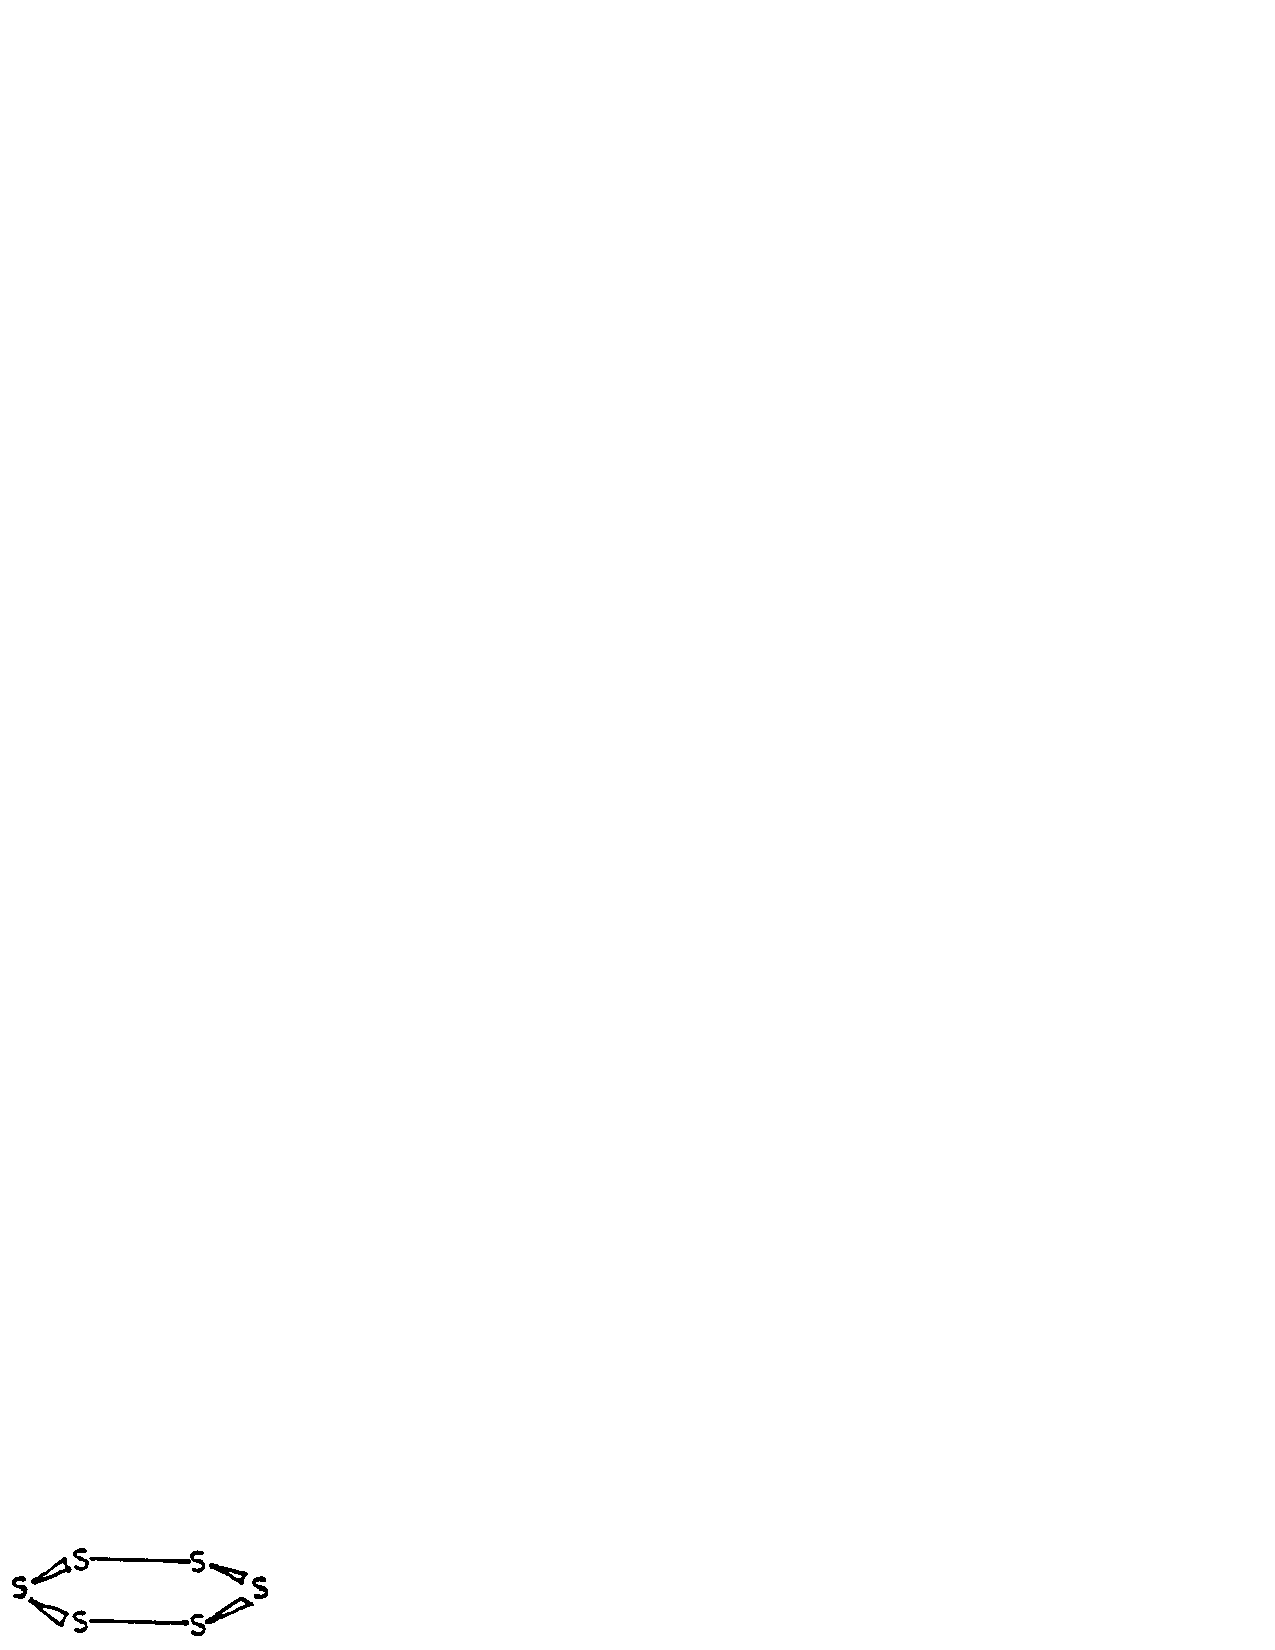
\includegraphics{fg12-34}
\end{equation}
with bond length 2.057 $\pm$ 0.018 \AA, bond angle 102.2 $\pm$
1.6$^{\circ}$, dihedral angle 74.5 $\pm 2.5^{\circ}$,
and packed so that each S$_6$ has van der Waals contacts with twelve other 
molecules.  Each atom has two neighbors at 3.50 \AA\ and one at 3.53 
\AA.  The vapor of this form consists of S$_6$ molecules.  An
orthorhombic form with S$_{12}$ rings, two per cell, has been found, 
and there is also another monoclinic form consisting of S$_8$ rings, 
the $\gamma$ form.  A fibrous sulfur with parallel infinite spirals,
ten atoms per three turns, also can be formed.

In this section, we have described the condensed phases of S, Se, Te, and Po 
in order to provide some idea of the variety of properties that can result 
for systems involving the same valence electron structure.  For S, Se, and 
Te the divalent character dominate; however, there are increasing effects 
due to more complicated bonding interactions.  Particularly for S, there are
several stable ring geometries leading to a variety of condensed forms.

\subsubsection{Thermochemistry}

The energetics for various forms of S, Se, and Te are listed in Table 
\ref{chap12-tab13}.  Some thermodynamic quantities are given in Table
\ref{chap12-tab14}.  Average  bond lengths and bond energies for O, S,
Se, and Te are tabulated in Table \ref{chap12-tab15}. The trends are
fairly uniform with the following exceptions.

The strength of a sigma bond increases from Te to Se to S, but decreases 
dramatically for O, whereas the pi bond increases slightly from Te to Se 
to S, but increases dramatically for O.  We attribute this to the
much higher overlap between pi orbitals on adjacent O, as compared to the 
other systems, partly due to the smaller bond length.  As a result, the 
pi bond, when it can be made, is very strong, and when these pi
orbitals are used in bonds to other ligands, the repulsive bond-bond 
interactions are very large.

The bond length changes are not monotonic.  That is, the change in the 
single bond length from S to Se, 0.28\AA, is much smaller than that 
from O to S, 0.60 \AA, or from Se to Te, 0.47 \AA.  This is because
there is a dramatic difference between S and Se.  Se has a filled $3d$ shell 
whereas S does not.  Since the $4s$ and $4p$ orbitals penetrate the $3d$ 
case somewhat, they are relatively more strongly bound than the $3s$ and
$3p$ orbitals of S leading to smaller orbitals than would otherwise have been 
expected from the sequence $2p \rightarrow 3p \rightarrow 4p$.  The same 
extra penetration occurs for Te, so that the increase in, size from Se to Te is
large again.  The decrease in the bond length upon making the pi bond 
is fairly constant; 0.25 \AA\ for O, 0.17 \AA\ for S, 0.17 \AA\ for 
Se, and 0.15 \AA\ for Te.


\begin{table}
\caption{Cohesive energies per atom, in kcal.}
\label{chap12-tab13}
\begin{tabular}{ccccc}\\ \hline
& & 298$^{\circ}$K$^a$ & 298$^{\circ}$K$^b$ & 0$^{\circ}$K\cr

S & orthorhombic & 66.636\cr
& monoclinic & 66.556\cr
S$_6$ & gas phase & 62.23\cr
S$_8$ & gas phase & 63.58\cr
Se & hexagonal,$^c$ black & 54.27\cr
& monoclinic, red & 52.7\cr
& amorphous & 53.1\cr
Se$_6$ & gas phase & 47.8\cr
Te & hexagonal,$^c$ & 47.02 & 46.91 & 46.89\cr
& amorphous & 44.3\cr
\hline
\end{tabular}\\
$^a$Reference 1.
$^b$Reference 2.
$^c$Metallic.
\end{table}

\begin{table}
\caption{}
\label{chap12-tab14}
\begin{tabular}{ccccccc}\\ \hline
&\multicolumn{2}{c}{Transitions}&\multicolumn{2}{c}{Melting}
&\multicolumn{2}{c}{Boiling}\cr
& T & $\Delta$H&T$_{mp}$ & $\Delta$H$_m$ & T$_{bp}$ & $\Delta$H$_v$\cr
& (K) & (kcal) & (K) & (kcal) & (K) & (298$^{\circ}$K)\cr

S~~~$\alpha \beta$ &368.54&0.0960&388.36&0.4105&717.75&3.145\cr
Se & & & 494 & 1.60 & 958 & 2.700$^{a,c}$\cr
Te & & & 722.65 & 4.18 & 1261 & 20.12$^b$\cr
\hline
\end{tabular}\\
$^a$Leads to M$_8$ molecules. 
$^b$Leads to M$_2$ molecules. 
$^c$625$^{\circ}$K.
\end{table}

\begin{table}
\caption{Bond length, in \AA, and bond energy, in kcal.}
\label{chap12-tab15}
\begin{tabular}{ccccccc}\\ \hline
&\multicolumn{3}{c}{Bond Length} &\multicolumn{3}{c}{Bond Energy}\cr
& Single & Sesqui & Double & $\sigma$ & $\pi^d$ & 1/2$\pi$\cr

O & 1.46 & 1.34 & 1.21 & 48 & 70 & 13\cr
S & 2.06 & & 1.89 & 64 & 39\cr
Se & 2.34 & & 2.17 & 50$^b$ & 29\cr
Te & 2.81$^a$ & & 2.56 & 43$^c$ & 19\cr
\hline
\end{tabular}\\
$^a$ Se leads to 2.34 \AA\ for gas phase Se$_6$ and the Se$_8$ rings of 
the $\alpha$ form, but 2.37 \AA\ for metallic Se. Thus, for Te we subtract 
0.03 \AA\ from the bond length, 2.835, in metallic Te.
$^b$ For S, the cohesive energy of the crystalline form is 66.6 kcal but the 
best estimate of the average single bond energy is 64 kcal, the value for 
gas phase S$_8$ is 63.6 kcal.  Thus, there is 2.6 kcal involved in other 
bonds.  For Se the cohesive energy for gas phase Se$_6$ is 47.8 kcal,
which is 14.4 kcal lower than the value for gas phase S$_6$.  Monoclinic Se 
has a cohesive energy 13. 8 kcal lower than that of monoclinic S. Thus, we 
take the sigma bond of Se to be 14 kcal weaker than that of S.
$^c$ For Te, the cohesive energy of metallic Te is 7.2 kcal smaller than that 
of metallic Se.  Thus, we take the sigma bond of Te to be 7 kcal weaker 
than that of Se.
$^d$ Calculated as the bond energy of the diatomic molecule minus the 
sigma bond energy in this table.
\end{table}



